%----------------------------------------------------------------------------------------
%	THESIS CONTENT - CHAPTERS
%----------------------------------------------------------------------------------------

\mainmatter % Begin numeric (1,2,3...) page numbering

\pagestyle{fancy} % Return the page headers back to the "fancy" style

% Include the chapters of the thesis as separate files from the Chapters folder
% Uncomment the lines as you write the chapters



\newcommand{\wglobal}{\textit{global}}
\newcommand{\wlocal}{\textit{local}}
\newcommand{\WGlobal}{$w_{\wglobal}^{*}$}
\newcommand{\WLocal}{$w_{\wlocal}^{*}$}

\newcommand{\PCAfull}{Piecewise Constant Approximation (PCA)}
\newcommand{\APCAfull}{Adaptive Piecewise Constant Approximation (APCA)}
\newcommand{\PWLHfull}{PieceWise Linear Histogram (PWLH)}
\newcommand{\CAfull}{Critical Aperture (CA)}
\newcommand{\SFfull}{Slide Filter (SF)}
\newcommand{\FRfull}{Fractal Resampling (FR)}
\newcommand{\GAMPSfull}{Grouping and AMPlitude Scaling (GAMPS)}

\newcommand{\dataCite}{\cite{dataset:irkis, dataset:sst1, dataset:elnino, dataset:solar, dataset:spc}}



\setstretch{1.1}

\chapter{Introduction} % Main chapter title
\label{intro:intro} % For referencing the chapter elsewhere, use \ref{Chapter1} 

\lhead{Chapter 1. \emph{Introduction}} % This is for the header on each page - perhaps a shortened title

\newcommand{\maxerror}{\textit{$\epsilon$}\xspace}
\newcommand{\alOne}{a_1}
\newcommand{\alTwo}{a_2}
\newcommand{\MaskVar}[1]{$\text{{#1}}_\textit{M}$}
\newcommand{\NonMaskVar}[1]{$\text{{#1}}_\textit{NM}$}
\newcommand{\win}{\textit{w}}

\newcommand{\RD}{\textnormal{RD}}
\newcommand{\RDit}{\textit{RD}}
\newcommand{\CRit}{\textit{CR}}
\newcommand{\CR}{\textnormal{CR}}

\newcommand{\zetafoot}{\footnote{A \textit{zettabyte (ZB)} is a unit of measurement of the size of digital information on a computer or other electronic device, which is equivalent to $10^{12}$ GB.} }


In the last 20 years, we have witnessed a staggering development of mobile communications and the Internet. Both factors have contributed to an accelerated expansion of the digital universe. Researchers estimate that the amount of digital data, created and replicated worldwide, more than doubles every three years: it went from 4.4 ZB\zetafoot in 2013, to 33 ZB in 2018, and it is expected to reach 175 ZB by the year 2025 \cite{Digitalization1, Digitalization2}. In this context, research on data compression has become more relevant than ever.


Data compression techniques allow for the reduction of the number of bits needed to represent digital data. There are two types of compression algorithms: \textit{lossless} and \textit{lossy}. Lossless compression algorithms allow the original data to be perfectly reconstructed from the compressed data. On the other hand, lossy compression algorithms only allow to reconstruct an approximation of the original data, though they usually obtain better compression rates (i.e. the compressed data is represented using even a smaller number of bits).


Data compression is ubiquitous, with applications in industry as well as various branches of scientific research. It is worth mentioning a few examples, just to paint a picture of its broad scope:
\vspace{-5pt}
\begin{itemize}
\item All the multimedia data that is sent, from the servers of both music (e.g. Spotify, Apple Music) and video (e.g. Youtube, Netflix) streaming services, to an end user device, is compressed to optimize the bandwidth usage \cite{SpotifyApple, HEVC}. Something similar occurs with digital television, where signals are encoded in the source, and decoded in the receiver \cite{DTV}.

\item Voice and video calls made on \textit{VoIP (Voice over IP)} software, such as Zoom \cite{Zoom} or Skype \cite{Skype}, always require the implementation of compression techniques on every end user device, without which it would not be possible to maintain a real-time conversation with proper sound and video quality.

\item Digital cameras use different compression algorithms to reduce the size of the image files, which allows to decrease the storage and transmission costs. In general, the end user is able to select between a lossy compression algorithm (JPEG being the most popular one), and a lossless one (TIFF is one of the industry standards, but leading brands have their own algorithms) \cite{Nikon, Canon}. 

\item There is a great variety of general-purpose compression tools, which allow to losslessly compress any type of file. Among the most popular ones are gzip \cite{gzip} and WinRAR \cite{WinRAR}, which also allow to encrypt and split the compressed files. 

\item In the medicine field, some tests (e.g. EEG, ECG) require for a patient to wear a monitoring device that measures clinical diagnosis data and wirelessly broadcasts it to a remote storage device, for an extended period of time. In such cases, compression algorithms are used to compress the transmitted data, which reduces the amount of energy consumed by the monitoring device, thus extending battery life \cite{EEG, ECG}.

\item NASA's space missions involve transmitting information back to Earth from space probes in far away places, which requires a great amount of energy. In past missions to Mars and Pluto, using onboard compression algorithms allowed to save resources, such as energy, space, and money, which is crucial for making space exploration viable \cite{HPMars, Pluto}.

\item A \textit{Wireless Sensor Network (WSN)} consists of spatially distributed sensors that communicate wirelessly to collect data about the surrounding environment. They are used in a wide variety of environmental, health, industrial, and military applications \cite{WSNWiley, WSNList}. Since the sensors are often placed in remote locations, it is important that they use energy-efficient compression algorithms and communication protocols, so that their power consumption is optimized.
% They have gain new interest with the internet of things. \cite{WSNIoT}
\end{itemize}


\newcommand{\footExampleOne}{\footnote{In general, lossless compression is recommended for archival purposes, while lossy compression is suggested to optimize the bandwidth usage when transmitting data.}}
\newcommand{\footExampleTwo}{\footnote{In general, compression algorithms executed in a battery-run device tend to have low computational complexity, so that a small amount of energy is consumed during the compression process.}}
\newcommand{\footSampling}{\footnote{In the context of WSNs, we consider that each sensor, which records data corresponding to a single signal, represents a different channel.}}


Even though some kind of data compression technique is involved in each one of the examples presented above, which specific compression algorithm is used in each case depends on a variety of factors \cite{DCTSurvey}, such as the characteristics of the data, the desired compression rate, whether the data is going to be archived or transmitted\footExampleOne, and whether the energy resources are critical or not\footExampleTwo.


In this work, we focus on the compression of multichannel signals with irregular sampling rates and with data gaps. There is a wide range of research on compression algorithms for multichannel signals with \textit{regular sampling rates} (see, for example, \cite{ImageOne, ImageTwo} for images, \cite{AudioOne, AudioTwo} for audio, \cite{VideoOne, VideoTwo} for video, and \cite{MedicalOne, MedicalTwo} for biomedical signals). However, real-world datasets sometimes consist of multichannel signals with \textit{irregular sampling rates}. This occurs frequently in datasets gathered by WSNs\footSampling, since different groups of sensors may be out of sync, and some might even malfunction. It is also common that errors arise when acquiring, transmitting or storing the data, causing a \textit{data gap}. Nevertheless, state-of-the-art algorithms designed for sensor data compression reported in the literature \cite{AnEva2013, Signal2016} assume, in general, that the signals have regular sampling rates and that there are no gaps in the data. Thus, in this thesis we design and implement a number of variants of state-of-the-art algorithms, adapt them so they are able to encode multichannel signals with irregular sampling rates and data gaps, and then evaluate their compression performance experimentally.


To assess the performance of our implemented algorithm variants, we consider eight different real-world datasets: dataset IRKIS \cite{dataset:irkis} is gathered by multiple soil moisture measuring sensors installed along the Dischma valley, in the municipality of Davos, Switzerland; datasets ElNino \cite{dataset:elnino}, SST and ADCP \cite{dataset:sst1} consist of various oceanographic and surface meteorological readings, obtained by sensors placed in buoys and moorings in the Pacific Ocean; dataset Solar \cite{dataset:solar} consists of solar radiation measurements in the city of Miami, Florida, US; and datasets Hail, Tornado and Wind \cite{dataset:spc} consist of data related to thunderstorms and tornadoes along US territory. Each experimental dataset consists of multichannel signals with one or both of the characteristics we are interested in, namely, irregular sampling rate and data gaps. The number of gaps, as well as other characteristics (e.g. whether they are smooth or rough signals, the number of outliers, periodicity), varies among different signals, which allows us to analyze the performance of the evaluated algorithms under different circumstances. The datasets come from multiple sources \dataCite, each using a different data representation format. Thus, as a first step, we transformed the data into a uniform format, which we define ourselves, and can be easily adapted to represent different kinds of datasets. The details of this data format, as well as the description of the experimental datasets, laying out the source, characteristics and relevant statistics of every signal involved, are presented in \textbf{Chapter~\ref{datasets}}.


Both the original and our implemented variants are \textit{near-lossless} compression algorithms. This type of algorithms guarantee a bounded per-sample absolute error between the decompressed and the original signals. The error threshold can be specified via a parameter, denoted~$\maxerror$. When $\maxerror$ is equal to zero, the compression is lossless, i.e., the decompressed and the original signals are identical. Additionally, the original algorithms and our proposed variants follow a model-based compression approach that compresses signals by exploiting correlation between signal samples taken at close times (\textit{temporal correlation}) and, in some cases, between samples from different channels (\textit{spatial correlation}). In addition to efficient compression performance, they offer some data processing features, like inferring uncertain sensor readings, detecting outliers, indexing, etc. \cite{AnEva2013}. The model-based techniques are classified into different categories, depending on the type of model: \textit{constant models} approximate signals by piecewise constant functions, \textit{linear models} use linear functions, and \textit{correlation models} simultaneously encode multiple signals exploiting temporal and spatial correlation. There also exist \textit{nonlinear models}, which approximate signals by nonlinear functions, but known algorithms that follow this technique do not support near-lossless compression and yield poor compression results~\cite{AnEva2013}. In total, we implement variants for eight different compression algorithms: \textit{\PCAfull} \cite{coder:pca} and \textit{\APCAfull} \cite{coder:apca}, which are constant model algorithms; \textit{\PWLHfull} \cite{coder:pwlh}, \textit{PWLHInt} (see Subsection~\ref{algo:pwhl:int}), \textit{\CAfull} \cite{coder:ca}, \textit{\SFfull} \cite{coder:sf}, and \textit{\FRfull} \cite{coder:fr}, which are linear model algorithms; and \textit{\GAMPSfull} \cite{coder:gamps}, which is a correlation model algorithm. The variants implemented for our evaluation are presented in \textbf{Chapter~\ref{algo}}, including a description of their parameters, details of their coding and decoding routines, and examples that show the encoding process step by step.


For most algorithms we design and implement two variants, \textit{masking (\maskalgo)} and \textit{non-masking (\NOmaskalgo)}, which differ in the encoding of the gaps in the data. Variant \maskalgo of an algorithm first encodes the position of all the gaps, and then proceeds to encode the data values separately, while variant \NOmaskalgo encodes the gaps and the data values together. The proposed strategy to compress the gaps in variant \maskalgo, which is presented in Section~\ref{algo:maskmodes}, uses arithmetic coding \cite{ac2, Cover2005} combined with a Krichevsky-Trofimov probability assignment \cite{ktestimator} over a Markov model. We point out that, with both variants, the gaps in a decompressed signal match the gaps in the original signal exactly, regardless of the value of the error threshold parameter (\maxerror). Efficient compression of gap information, especially in variant \maskalgo, is an original contribution of this thesis.


In \textbf{Chapter~\ref{experiments}} we present and analyze a series of experimental results, with the aim of evaluating and comparing the various tested algorithm variants in practical scenarios. All of our experiments involve the compression of data obtained from the real-world datasets presented in Chapter~\ref{datasets}. We assess the compression performance of an algorithm variant through the \textit{compression ratio (CR)}, which is calculated by the formula
\vspace{-2pt}
\begin{equation}
\CR = \frac{\textnormal{size of compressed data}}{\textnormal{size of original data}}.
\end{equation}


\clearpage


Thus, smaller values of CR correspond to a better performance. To compare the compression performance between two algorithm variants $\alOne$ and $\alTwo$, we consider the \textit{relative difference (RD)} metric, which is calculated by the formula
\vspace{-2pt}
\newcommand{\sizeofd}{\textnormal{size of data compressed with }}
\begin{equation}
\RD(\alOne, \alTwo) = 100\times\frac{\sizeofd \alTwo - \sizeofd \alOne}{\sizeofd \alTwo}.
\end{equation}

\vspace{-2pt}
Therefore, $\alOne$ has a better performance than $\alTwo$ iff $\RD(\alOne, \alTwo)$ is positive.


\newcommand{\footSupportBoth}{\footnote{Algorithms SF and FR only support variant \maskalgo, while the rest of the algorithms support variants \maskalgo and \NOmaskalgo.}}


In Section~\ref{secX:rendimiento-relativo}, for each algorithm $a$ that supports variants \maskalgo and \NOmaskalgo\footSupportBoth, we compare the respective compression performance of both, $a_\maskalgo$ and $a_\NOmaskalgo$. The results show that on datasets with few or no gaps the performance of both variants is roughly the same, i.e. $\RD(a_\maskalgo, a_\NOmaskalgo)$ is always close to zero, ranging between $-0.29$ and $1.76\%$. On the other hand, on datasets with many gaps variant \maskalgo always performs better, in some cases with a significant difference, with $\RD(a_\maskalgo, a_\NOmaskalgo)$ ranging between $2.44$ and $50.78\%$. These experimental results suggest that variant \maskalgo is more robust and performs better in general.


\newcommand{\footSupportFocus}{\footnote{\label{note1}Due to the results obtained in Section~\ref{secX:rendimiento-relativo}, our experiments in the subsequent sections in Chapter~\ref{experiments} focus on studying the compression performance of variant \maskalgo of the algorithms.}}


Every original algorithm (and its respective variants) depends on a window size parameter, denoted $\win$, which defines the size of the windows into which the data are partitioned for encoding. In algorithm PCA, it defines a \textit{fixed window size}, while in the rest of the algorithms it defines a \textit{maximum window size}. In Section~\ref{secX:windows} we analyze the sensitivity of variant \maskalgo of each algorithm\footSupportFocus\ to this parameter. For each dataset, we compress each data file, and compare the results obtained when using a window size optimized for said specific file, against the results obtained when using a window size optimized for the whole dataset. The results indicate that the difference in compression performance is generally rather small, with the RD being less than or equal to $2\%$ in $97.7\%$ of the experimental cases. Therefore, we could fix the window size parameter in advance, for example by optimizing over a training set, without significantly compromising the overall performance of the compression algorithm variant. This is relevant, since obtaining the optimal window size for a specific data file is, in general, computationally expensive.


The last part of our experimental analysis, which is presented in Section~\ref{secX:codersmask}, consists in comparing the compression performance of our adapted algorithm variants, with each other, and with the general-purpose lossless compression algorithm gzip \cite{gzip}. Taking into account the discussion in the previous two paragraphs, for this analysis we only consider variant \maskalgo of each algorithm, and in every case we use the optimal window size for each whole dataset. Our experimental results indicate that none of the algorithm variants obtains the best compression performance in every scenario. This means that the optimal selection of a variant depends on the characteristics of the data to be compressed, and the error threshold ($\maxerror$) that is allowed. In some circumstances, even a general-purpose compression algorithm such as gzip outperforms the specific variants. Nevertheless, we extract some general conclusions from our analysis. For large error thresholds, variant \MaskVar{APCA} achieves the best compression results, obtaining the minimum CR in 76 out of 84 experimental cases ($90.5\%$). On the other hand, algorithm gzip and variant \MaskVar{PCA} are preferred for lower thresholds scenarios, since they obtain the minimum CR in 18 and 17 out of 42 experimental cases ($42.9\%$ and $40.5\%$), respectively.


Finally, in \textbf{Chapter~\ref{conclusions}} we sum up the conclusions of our thesis, and we propose some ideas to carry out as future work.


% Chapter ?

\chapter{Datasets} % Main chapter title
\label{datasets} % For referencing the chapter elsewhere, use \ref{Chapter1} 

\lhead{Chapter 2. \emph{Datasets}} % This is for the header on each page - perhaps a shortened title



\newcommand{\datasetirkis}{IRKIS}
\newcommand{\datasetsst}{SST}
\newcommand{\datasetadcp}{ADCP}
\newcommand{\datasetsolar}{Solar}
\newcommand{\datasetelnino}{ElNino}
\newcommand{\datasethail}{Hail}
\newcommand{\datasettornado}{Tornado}
\newcommand{\datasetwind}{Wind}

\newcommand{\datasetsolarcols}{GHI, DNI, DHI}
\newcommand{\datasetelninocols}{Lat, Long, Zon.Wind, Mer.Wind, Humidity, Air Temp., SST}
\newcommand{\datasethailcols}{Lat, Long, Size}
\newcommand{\datasettornadocols}{Lat, Long}
\newcommand{\datasetwindcols}{Lat, Long, Speed}







\newcommand{\BeCe}{B_c}


In this chapter we introduce the datasets used in our experiments. Every dataset consists of signals with one or both of the characteristics we are interested in, namely, irregular sampling rate and data gaps. In Chapter~\ref{experiments}, we present our experimental results, which make use of these datasets to analyze the compression performance of our implemented algorithm variants, which are presented in Chapter~\ref{algo}.


The datasets come from multiple sources \dataCite, each using a different data representation format. We transformed the data into a consistent, uniform format, which can be easily adapted to represent different kinds of datasets. In \textbf{Section~\ref{datasets:over}} we describe this format, including an example file that illustrates how the data is represented. In \textbf{sections~\ref{datasets:irkis}} to \textbf{\ref{datasets:wind}} we present each of the eight real-world datasets, namely, IRKIS \cite{dataset:irkis}, SST, ADCP \cite{dataset:sst1}, ElNino \cite{dataset:elnino}, Solar \cite{dataset:solar}, Hail, Tornado, and Wind \cite{dataset:spc}, laying out the source, characteristics and relevant statistics of every signal involved. Finally, in \textbf{Section~\ref{datasets:summary}} we summarize the information presented in this chapter, specifying the number of files, the number of gaps, and the data types of each dataset, as well as the measuring unit, scale, and range of each data type.



\clearpage
\section{Data format}
\label{datasets:over}


The data from every dataset \dataCite\ was transformed to a consistent format, which can be adapted to represent different types of datasets. In Figure~\ref{datasets:table:csvexample} we present an example of a csv file with this format. Although a csv file is simply a delimited text file that uses commas to separate values, we display its contents in the form of a table for legibility. The first three rows have general data, namely a dataset unique name, in this example ElNino, the measure unit for signal timestamps, and the timestamp value for the first sample. The fourth row has the labels of the data columns, and the remaining rows consist of the actual signal data.




\begin{table}[h]
\vspace{+5pt}
\begin{center}
    \begin{tabular}{| C{2.3cm} | C{2.3cm} | C{1.63cm} |  C{2cm} |  C{2cm} |  C{1.62cm} |}
    \hline
      \multicolumn{1}{|>{\centering\arraybackslash}m{2.3cm}|}{DATASET:}
    & \multicolumn{1}{>{\centering\arraybackslash}m{2.3cm}|}{ElNino} 
    & \multicolumn{1}{>{\centering\arraybackslash}m{1.63cm}|}{} 
    & \multicolumn{1}{>{\centering\arraybackslash}m{2cm}|}{}
    & \multicolumn{1}{>{\centering\arraybackslash}m{2cm}|}{}
    & \multicolumn{1}{>{\centering\arraybackslash}m{1.62cm}|}{}\\
    \hline
DATA ROWS:       & 7                &         &             &                         &         \\\hline
FIRST TIMESTAMP: & 1980-03-07 00:00:00 &         &             &                         &         \\\hline
METADATA:       &                 &         &             &             &                     \\\hline
COLUMNS   & UNIT             & SCALE & MINIMUM & MAXIMUM &                     \\\hline
Time Delta & hours              & 1      & 0        & 131071   &                     \\\hline
Lat        & coord. degrees & 100    & -1000    & 1000     &                     \\\hline
Long       & coord. degrees & 100    & -18000   & 18000    &                     \\\hline
Mer. Wind  & m/s               & 10     & -150     & 150      &                     \\\hline
Air Temp.  & °C                 & 100    & 0        & 4000     &                     \\\hline
Sea Temp.  & °C                 & 100    & 0        & 4000     &                     \\\hline
DATA:       &                 &         &             &             &                     \\\hline
Time Delta       & Lat                 & Long     & Mer. Wind     & Air Temp.  & Sea Temp.     \\\hline
\ 0              & -2                  & -10946   & \ 7         & 2614       & 2624    \\\hline
24               & -2                  & -10946   & 11          & \ \ \ N    & \ \ \ N \\\hline
24               & -2                  & -10946   & 22          & \ \ \ N    & \ \ \ N \\\hline
48               & -1                  & -10946   & 19          & \ \ \ N    & 2431    \\\hline
24               & -2                  & -10946   & 15          & 2557       & 2319    \\\hline
48               & -2                  & -10946   & \ 3         & 2472       & 2364    \\\hline
24               & -2                  & -10946   & -1         & \ \ \ N    & 2434    \\\hline
    \toprule[0.1mm]
    \end{tabular}
    \caption{Example of a dataset CSV file with the format we defined.}
    \label{datasets:table:csvexample}
\end{center}
\end{table}



\vspace{-5pt}
The values in the first data column, which we label ``Time Delta'', represent the timestamps associated with the data from the rest of the columns. We often refer to this column as the timestamp column. It is always the first column, and it is present in every csv file. In practice, this timestamp may represent the time at which the data was read, transmitted, stored, etc. Each but the first timestamp is represented as an integer value, which is an increment with respect to the previous timestamp, measured in the unit specified in the second row. As mentioned, the value of the first timestamp is given in the third row. In the example presented in Figure~\ref{datasets:table:csvexample}, the first four timestamps are ``1980-03-07 00:00:00'', ``1980-03-08 00:00:00'', ``1980-03-09 00:00:00'', and ``1980-03-11 00:00:00''. Notice that the difference between subsequent timestamps is not constant, varying between 24 and 48 hours, which means that the signals in this dataset have irregular sampling (recall that this is one of the characteristics we are interested in).


Besides the timestamp column, the csv presented in Figure~\ref{datasets:table:csvexample} consists of six additional data columns, each representing a different data type. The first two columns represent the latitude and longitude coordinates, respectively, of a buoy floating in the ocean, while the last four columns represent readings of various physical magnitudes (wind velocity, air temperature, and sea temperature), made by sensors set in the buoy. In general, the timestamp column can only consist of integer values, while the rest of the columns can have both integer values and the character ``N". An integer value represents an actual data sample, whose range depends on the range and accuracy of the sampling instrument used for acquiring and storing the data, while character ``N" represents a gap in the data. In practice, this data gap may occur when there's an error acquiring, transmitting or storing the data. In the example in Figure~\ref{datasets:table:csvexample}, there are some gaps in the last two data columns (recall that this is another of the characteristics we are interested in).



\clearpage
\section{Dataset IRKIS}
\label{datasets:irkis}


Dataset IRKIS \cite{dataset:irkis} consists of soil moisture measurements from stations installed along the Dischma valley, in the municipality of Davos, Switzerland, in the period between October 2010 and October 2013. This information is particularly useful to researchers who study the role of soil moisture in relation with the snowpack runoff and catchment discharge in high alpine terrain \cite{dataset:irkis2}. 


The dataset corresponds to seven stations, labeled 1202, 1203, 1204, 1205, 222, 333, and SLF2, which can be located in the map presented in~\cite{dataset:irkis}. For each station, the dataset contains measures of soil moisture data at different depths below the surface, namely 10, 30, 50, 80 and 120 cm. For each depth, there are moisture measures coming from two sensors, labeled A and B in the dataset files. Thus, for each station, there are 10 different data samples stored for each timestamp. The sensors measure the \textit{Volumetric Water Content (VWC)}, which is equal to the ratio of water volume to soil volume. Therefore, higher VWC values indicate a more moist soil. The original sample values have a precision of three significant figures, so they are transformed into the integer domain by multiplying them by $10^3$. 


\newcommand{\commonTable}{The first three columns show the total number of rows, columns and entries (i.e. number of rows times number of columns), respectively. The fourth column specifies the number of gaps, and the percentage of gaps over the total number of entries. The last five columns show the minimum, maximum, median, mean, and standard deviation, of the sample values }


In Table~\ref{datasets:table:irkis} we present some statistics of dataset IRKIS. The data from each station is stored in a separate csv file, and every row in the table contains statistics of a different file. \commonTable (dimensionless).



\begin{table}[h]
\vspace{+5pt}
\begin{center}
    \begin{tabular}{| C{1.2cm} || C{1.2cm} | C{1cm} |  C{1.5cm} |  C{2.2cm} | C{0.7cm} | C{0.7cm} | C{0.7cm} | C{0.9cm} | C{0.9cm} |}
    \hline
      \multicolumn{1}{|>{\centering\arraybackslash}m{1.2cm}||}{\textbf{Station}}
    & \multicolumn{1}{>{\centering\arraybackslash}m{1.2cm}|}{\textbf{\#Rows}} 
    & \multicolumn{1}{>{\centering\arraybackslash}m{1cm}|}{\textbf{\#Cols}} 
    & \multicolumn{1}{>{\centering\arraybackslash}m{1.5cm}|}{\textbf{\#Entries}}
    & \multicolumn{1}{>{\centering\arraybackslash}m{2.2cm}|}{\textbf{\#Gaps (\%)}}
    & \multicolumn{1}{>{\centering\arraybackslash}m{0.7cm}|}{\textbf{Min}}
    & \multicolumn{1}{>{\centering\arraybackslash}m{0.7cm}|}{\textbf{Max}}
    & \multicolumn{1}{>{\centering\arraybackslash}m{0.7cm}|}{\textbf{Mdn}}
    & \multicolumn{1}{>{\centering\arraybackslash}m{0.9cm}|}{\textbf{Mean}}
    & \multicolumn{1}{>{\centering\arraybackslash}m{0.9cm}|}{\textbf{SD}}\\
    \hline
%% SCRIPT OUTPUT BELOW HERE
1202 & 26,305 & 10 & 263,050 & 125,190 (47.6) & 240 & 541 & 428 & 417.1 & \ \ 48.8 \\\hline
1203 & 26,305 & 10 & 263,050 & 200,051 (76.1) & 165 & 385 & 249 & 257.7 & \ \ 40.1 \\\hline
1204 & 26,305 & 10 & 263,050 & 178,657 (67.9) & 218 & 464 & 298 & 313.3 & \ \ 70.0 \\\hline
1205 & 26,305 & 10 & 263,050 & 224,287 (85.3) & 272 & 600 & 315 & 342.1 & \ \ 63.9 \\\hline
222 & 26,304 & 10 & 263,040 & \ \ 56,007 (21.3) & 128 & 562 & 426 & 384.2 & 119.7 \\\hline
333 & 26,088 & 10 & 260,880 & \ \ 37,520 (14.4) & \ \ 38 & 451 & 327 & 291.5 & \ \ 81.1 \\\hline
SLF2 & 26,305 & 10 & 263,050 & \ \ 43,049 (16.4) & 215 & 580 & 352 & 360.9 & \ \ 65.1 \\\hline
%% SCRIPT OUTPUT ABOVE HERE
    \toprule[0.1mm]
    \end{tabular}
    \caption{Number of rows, columns, entries and gaps (total and percentual), and minimum, maximum, median, and standard deviation, of the sample values (dimensionless), for each file of the dataset IRKIS. The gaps are ignored when calculating the median, mean and standard deviation.}
    \label{datasets:table:irkis}
\end{center}
\end{table}






\vspace{-10pt}
\section{Dataset SST}
\label{datasets:sst}
\newcommand{\TAODef}{This dataset is collected by the Tropical Atmosphere Ocean (TAO) project, which was established in 1985 to study annual climate variations near the equator \cite{dataset:tao}.}

Dataset SST \cite{dataset:sst1} consists of \textit{Sea Surface Temperature (SST)} measurements from buoys floating in the Pacific Ocean. \TAODef


The dataset consists of readings from 55 buoys, which can be located in the map presented in \cite{dataset:sst1}. For each timestamp, the dataset contains the SST measurement taken in each buoy. Thus, a total of 55 data samples are stored for each timestamp. The temperature is measured in degree Celsius (°C), with a precision of three significant figures. Every sample value is transformed to the integer domain by multiplying it by $10^3$.


\clearpage


In Table~\ref{datasets:table:sst} we present some statistics of dataset SST. The data for each month is stored in a separate csv file, and every row in the table contains statistics of a different file. \commonTable (in °C).



\begin{table}[h]
\vspace{+5pt}
\begin{center}
    \begin{tabular}{| C{1.2cm} || C{1.1cm} | C{1cm} |  C{1.5cm} |  C{2.02cm} | C{0.55cm} | C{0.98cm} | C{0.98cm} | C{1.25cm} | C{1.08cm} |}
    \hline
      \multicolumn{1}{|>{\centering\arraybackslash}m{1.2cm}||}{\textbf{Month}}
    & \multicolumn{1}{>{\centering\arraybackslash}m{1.1cm}|}{\textbf{\#Rows}} 
    & \multicolumn{1}{>{\centering\arraybackslash}m{1cm}|}{\textbf{\#Cols}} 
    & \multicolumn{1}{>{\centering\arraybackslash}m{1.5cm}|}{\textbf{\#Entries}}
    & \multicolumn{1}{>{\centering\arraybackslash}m{2.02cm}|}{\textbf{\#Gaps (\%)}}
    & \multicolumn{1}{>{\centering\arraybackslash}m{0.55cm}|}{\textbf{Min}}
    & \multicolumn{1}{>{\centering\arraybackslash}m{0.98cm}|}{\textbf{Max}}
    & \multicolumn{1}{>{\centering\arraybackslash}m{0.98cm}|}{\textbf{Mdn}}
    & \multicolumn{1}{>{\centering\arraybackslash}m{1.25cm}|}{\textbf{Mean}}
    & \multicolumn{1}{>{\centering\arraybackslash}m{1.08cm}|}{\textbf{SD}}\\
    \hline
%% SCRIPT OUTPUT BELOW HERE
01-2017 & 4,392 & 55 & 241,560 & 92,866 (38.4) & 3 & 32,367 & 27,221 & 27,326.9 & 2,406.0 \\\hline
02-2017 & 3,984 & 55 & 219,120 & 84,292 (38.5) & 3 & 31,277 & 27,477 & 27,677.3 & 1,953.1 \\\hline
03-2017 & 4,362 & 55 & 239,910 & 99,541 (41.5) & 3 & 31,809 & 28,070 & 28,050.9 & 1,760.4 \\\hline
%% SCRIPT OUTPUT ABOVE HERE
    \toprule[0.1mm]
    \end{tabular}
    \caption{Statistics of dataset SST for each month. The gaps are ignored when calculating the median, mean and standard deviation of the sample values.}
    \label{datasets:table:sst}
\end{center}
\end{table}





\vspace{-20pt}
\section{Dataset ADCP}
\label{datasets:adcp}


\vspace{-5pt}
Dataset ADCP \cite{dataset:sst1} consists of water current velocity measurements from moorings in the Pacific Ocean. \TAODef


The dataset consists of readings from 3 moorings, which can be located in the map presented in \cite{dataset:sst1}. In each mooring, readings are made by a total of 63 \textit{acoustic Doppler current profilers (ADCPs)}, placed at different depths below the ocean. Each ADCP measures the \textit{eastward (UCUR)}, \textit{northward (VCUR)}, and \textit{upward (WCUR)} components of the water current velocity. Therefore, there are 567 ($3\times63\times3$) data samples stored for each timestamp. The velocity is measured in m/s, and its scale is $10^3$.


In Table~\ref{datasets:table:adcp} we present some statistics of dataset ADCP. The data for each month is stored in a separate CSV file, and every row in the table contains statistics for one such file. \commonTable (in m/s).


% \vspace{-10pt}

\begin{table}[h]
\vspace{+5pt}
\begin{center}
    \begin{tabular}{| C{1.18cm} || C{0.78cm} | C{0.78cm} |  C{1.18cm} |  C{2.2cm} | C{0.7cm} | C{0.88cm} | C{0.590cm} | C{0.9cm} | C{0.9cm} |}
    \hline
      \multicolumn{1}{|>{\centering\arraybackslash}m{1.18cm}||}{\fsi\textbf{Month}}
    & \multicolumn{1}{>{\centering\arraybackslash}m{0.78cm}|}{\fsi\textbf{Rows}} 
    & \multicolumn{1}{>{\centering\arraybackslash}m{0.78cm}|}{\fsi\textbf{Cols}} 
    & \multicolumn{1}{>{\centering\arraybackslash}m{1.18cm}|}{\fsi\textbf{Entries}}
    & \multicolumn{1}{>{\centering\arraybackslash}m{2.2cm}|}{\fsi\textbf{Gaps (\%)}}
    & \multicolumn{1}{>{\centering\arraybackslash}m{0.7cm}|}{\fsi\textbf{Min}}
    & \multicolumn{1}{>{\centering\arraybackslash}m{0.88cm}|}{\fsi\textbf{Max}}
    & \multicolumn{1}{>{\centering\arraybackslash}m{0.590cm}|}{\fsi\textbf{Mdn}}
    & \multicolumn{1}{>{\centering\arraybackslash}m{0.9cm}|}{\fsi\textbf{Mean}}
    & \multicolumn{1}{>{\centering\arraybackslash}m{0.9cm}|}{\fsi\textbf{SD}}\\
    \hline
%% SCRIPT OUTPUT BELOW HERE
01-2015 & 744 & 567 & 421,848 & 134,544 (31.9) & -805 & 1,394 & 6 & 113.7 & 273.1 \\\hline
02-2015 & 672 & 567 & 381,024 & 125,151 (32.8) & -761 & 1,822 & 7 & 154.5 & 318.3 \\\hline
03-2015 & 744 & 567 & 421,848 & 133,110 (31.6) & -870 & 2,094 & 13 & 185.5 & 367.4 \\\hline
%% SCRIPT OUTPUT ABOVE HERE
    \toprule[0.1mm]
    \end{tabular}
    \caption{\tableExplain{in m/s}{ADCP} \ignoredGaps}
    \label{datasets:table:adcp}
\end{center}
\end{table}



% \clearpage


% \vspace{-15pt}
\clearpage
\section{Dataset ElNino}
\label{datasets:elnino}

Dataset ElNino \cite{dataset:elnino} consists of various oceanographic and surface meteorological measurements from buoys floating in the Pacific Ocean between 1980 and 1998. \TAODef


The dataset consists of readings from 78 buoys, which move around in the Pacific Ocean, near the equator. For each timestamp, the position of each buoy is specified, in terms of its latitude and longitude (°), and in each buoy the following measurements are taken: speed of the zonal and meridional winds (m/s), relative humidity (\%), and air temperature and SST (°C). Therefore, a total of 546 ($78\times7$) data samples are stored for each timestamp. The original sample values for the latitude, longitude, air temperature, and SST, have a precision of two significant figures, so they are transformed into the integer domain by multiplying them by $10^2$. Instead, the original sample values for the speed of the zonal and meridional winds, and the relative humidity, have a precision of one significant figure, so they are transformed into the integer domain by multiplying them by $10$.


In Table~\ref{datasets:table:elnino} we present some statistics of dataset ElNino. The dataset consists of a single file, and each row in the table contains statistics concerning a different data type. The first column specifies the number of gaps, and the percentage of gaps over the total number of entries. The file has 6,371 rows, so there is a total of 496,938 ($78\times6,371$) entries of each data type. The rest of the columns show the minimum, maximum, median, mean, and standard deviation, of the sample values (in their respective units of measurement).



\begin{table}[h]
\vspace{+5pt}
\begin{center}
    \begin{tabular}{| C{3.36cm} || C{2.18cm} | C{1.13cm} | C{1.13cm} | C{1.13cm} | C{1.3cm} | C{1.25cm} |}
    \hline
      \multicolumn{1}{|>{\centering\arraybackslash}m{3.36cm}||}{\textbf{Data Type}}
    & \multicolumn{1}{>{\centering\arraybackslash}m{2.18cm}|}{\textbf{\#Gaps (\%)}}
    & \multicolumn{1}{>{\centering\arraybackslash}m{1.13cm}|}{\textbf{Min}}
    & \multicolumn{1}{>{\centering\arraybackslash}m{1.13cm}|}{\textbf{Max}}
    & \multicolumn{1}{>{\centering\arraybackslash}m{1.13cm}|}{\textbf{Mdn}}
    & \multicolumn{1}{>{\centering\arraybackslash}m{1.3cm}|}{\textbf{Mean}}
    & \multicolumn{1}{>{\centering\arraybackslash}m{1.25cm}|}{\textbf{SD}}\\
    \hline
%% SCRIPT OUTPUT BELOW HERE
Lat (coord. degrees) & 318,858 (64.2) & \ \ \ \ -881 & \ \ \ \ 905 & \ \ \ \ \ \ \ 1 & \ \ \ \ \ 47.3 & \ \ \ \ 458.2 \\\hline
Long (coord. degrees) & 318,858 (64.2) & -18,000 & 17,108 & -11,126 & -5,402.5 & 13,536.4 \\\hline
Zon. Wind (m/s) & 344,021 (69.2) & \ \ \ \ -124 & \ \ \ \ 143 & \ \ \ \ \ -40 & \ \ \ \ -33.0 & \ \ \ \ \ 33.7 \\\hline
Mer. Wind (m/s) & 344,020 (69.2) & \ \ \ \ -116 & \ \ \ \ 130 & \ \ \ \ \ \ \ 3 & \ \ \ \ \ \ 2.5 & \ \ \ \ \ 30.0 \\\hline
Humidity (\%) & 384,619 (77.4) & \ \ \ \ \ 454 & \ \ \ \ 999 & \ \ \ \ \ 812 & \ \ \ \ 812.4 & \ \ \ \ \ 53.1 \\\hline
Air Temp. (°C) & 337,095 (67.8) & \ \ \ 1,705 & \ \ 3,166 & \ \ \ 2,734 & \ \ 2,688.8 & \ \ \ \ 181.6 \\\hline
Sea Temp. (°C) & 335,865 (67.6) & \ \ \ 1,735 & \ \ 3,126 & \ \ \ 2,829 & \ \ 2,771.5 & \ \ \ \ 205.7 \\\hline
%% SCRIPT OUTPUT ABOVE HERE
    \toprule[0.1mm]
    \end{tabular}
    \caption{Number of gaps (total and percentual), and minimum, maximum, median, and standard deviation, of the sample values (in their respective units of measurement), for each data type of the dataset ElNino. \ignoredGaps}
    \label{datasets:table:elnino}
\end{center}
\end{table}





\vspace{-10pt}
\section{Dataset Solar}
\label{datasets:solar}
\newcommand{\unitSolar}{W/$\textnormal{m}^2$}

Dataset Solar \cite{dataset:solar} consists of solar radiation measurements from sensors in the city of Miami, Florida, US. This dataset is collected by SolarAnywhere, an online tool used for monitoring solar radiation around the world.


The dataset consists of readings from 12 sensors, where each sensor measures three different types of solar irradiance, namely, \textit{Global Horizontal Irradiance (GHI)}, \textit{Direct Normal Irradiance (DNI)}, and \textit{Diffuse Horizontal Irradiance (DHI)}. Thus, a total of 36 data samples are stored for each timestamp. The solar irradiance is measured in \unitSolar, with a precision of zero significant figures. Therefore, the sample values are in the integer domain and it is not necessary to transform them.


In tables \ref{datasets:table:solar1}, \ref{datasets:table:solar2}, \ref{datasets:table:solar3}, and \ref{datasets:table:solar4}, we present some statistics of dataset Solar for years 2011, 2012, 2013, and 2014, respectively. The data for each year is stored in a different csv file. Each file has 8,759 rows, with a total of 105,108 ($12\times8,759$) entries of each data type. Each row in the tables contains statistics concerning a different data type. The first column specifies the number of gaps, and the percentage of gaps over the total number of entries. The rest of the columns show the minimum, maximum, median, mean, and standard deviation, of the sample values (in \unitSolar).



\newcommand{\beginTableSolar}{
\begin{table}[h]
\vspace{+5pt}
\begin{center}
\begin{tabular}{| C{2cm} || C{2.5cm} | C{1.2cm} | C{1.2cm} | C{1.2cm} | C{1.4cm} | C{1.4cm} |}
\hline
  \multicolumn{1}{|>{\centering\arraybackslash}m{2cm}||}{\textbf{Data Type}}
& \multicolumn{1}{>{\centering\arraybackslash}m{2.5cm}|}{\textbf{\#Gaps (\%)}}
& \multicolumn{1}{>{\centering\arraybackslash}m{1.2cm}|}{\textbf{Min}}
& \multicolumn{1}{>{\centering\arraybackslash}m{1.2cm}|}{\textbf{Max}}
& \multicolumn{1}{>{\centering\arraybackslash}m{1.2cm}|}{\textbf{Mdn}}
& \multicolumn{1}{>{\centering\arraybackslash}m{1.4cm}|}{\textbf{Mean}}
& \multicolumn{1}{>{\centering\arraybackslash}m{1.4cm}|}{\textbf{SD}}\\
\hline
}

\newcommand{\finTableSolar}[2]{
\toprule[0.1mm]
\end{tabular}
\caption{Number of gaps (total and percentual), and minimum, maximum, median, and standard deviation, of the sample values (in \unitSolar), for each data type of the dataset Solar, for year {#2}. \ignoredGaps}
{#1}
\end{center}
\end{table}
}


\beginTableSolar
GHI & 23 (0.02) & 0 & 1,005 & \ 11 & 187.6 & 274.7 \\\hline
DNI & 23 (0.02) & 0 & \ \ \ 959 & \ \ 3 & 183.5 & 278.2 \\\hline
DHI & 23 (0.02) & 0 & \ \ \ 763 & \ \ 8 & \ \ 70.5 & \ \ 96.8 \\\hline
\finTableSolar{\label{datasets:table:solar1}}{2011}


\vspace{-10pt}
\beginTableSolar
GHI & 0 (0.0) & 0 & 1,004 & \ \ 9 & 186.0 & 269.7 \\\hline
DNI & 0 (0.0) & 0 & \ \ \ 958 & \ \ 3 & 178.3 & 272.8 \\\hline
DHI & 0 (0.0) & 0 & \ \ \ 485 & \ \ 7 & \ \ 72.7 & 100.4 \\\hline
\finTableSolar{\label{datasets:table:solar2}}{2012}

\vspace{-10pt}
\beginTableSolar
GHI & 156 (0.15) & 0 & 1,004 & \ \ 9 & 183.7 & 267.8 \\\hline
DNI & 156 (0.15) & 0 & \ \ \ 954 & \ \ 3 & 168.9 & 261.8 \\\hline
DHI & 156 (0.15) & 0 & \ \ \ 483 & \ \ 7 & \ \ 75.8 & 103.2 \\\hline
\finTableSolar{\label{datasets:table:solar3}}{2013}

\vspace{-10pt}
\beginTableSolar
GHI & 204 (0.19) & 0 & 1,006 & \ \ 9 & 189.5 & 274.8 \\\hline
DNI & 204 (0.19) & 0 & \ \ \ 959 & \ \ 4 & 181.0 & 274.6 \\\hline
DHI & 204 (0.19) & 0 & \ \ \ 473 & \ \ 7 & \ \ 73.1 & 100.1 \\\hline
\finTableSolar{\label{datasets:table:solar4}}{2014}





\vspace{-10pt}
\section{Dataset Hail}
\label{datasets:hail}
\newcommand{\SPCDef}{This dataset is collected by the Storm Prediction Center (SPC), a US government agency established in 1995, whose goal is to forecast the risk of severe thunderstorms and tornadoes along US territory.}

Dataset Hail \cite{dataset:spc} consists of hail size measurements from several stations around the US, taken between 2015 and 2017. \SPCDef


The dataset consists of hail diameter readings from several stations distributed around the US. For each timestamp, besides the hail diameter measurement, the position of the station where the measurement is taken is specified, in terms of its latitude and longitude (°). The hail diameter is measured in 1/100 of an inch, with a precision of zero significant figures, so the sample values are in the integer domain and it is not necessary to transform them.


\newcommand{\SPCTable}{The dataset consists of a single file, and each row in the table contains statistics concerning a different data type. The first column specifies the number of gaps, and the percentage of gaps over the total number of entries. }

In Table~\ref{datasets:table:hail} we present some statistics of dataset Hail. \SPCTable The file has 17,059 rows, so there is the same number of entries of each data type. The rest of the columns show the minimum, maximum, median, mean, and standard deviation, of the sample values (in their respective units of measurement).



\begin{table}[h]
\vspace{+5pt}
\begin{center}
    \begin{tabular}{| C{2cm} || C{2.5cm} | C{1.2cm} | C{1.2cm} | C{1.2cm} | C{1.4cm} | C{1.4cm} |}
    \hline
      \multicolumn{1}{|>{\centering\arraybackslash}m{2cm}||}{\textbf{Data Type}}
    & \multicolumn{1}{>{\centering\arraybackslash}m{2.5cm}|}{\textbf{\#Gaps (\%)}}
    & \multicolumn{1}{>{\centering\arraybackslash}m{1.2cm}|}{\textbf{Min}}
    & \multicolumn{1}{>{\centering\arraybackslash}m{1.2cm}|}{\textbf{Max}}
    & \multicolumn{1}{>{\centering\arraybackslash}m{1.2cm}|}{\textbf{Mdn}}
    & \multicolumn{1}{>{\centering\arraybackslash}m{1.4cm}|}{\textbf{Mean}}
    & \multicolumn{1}{>{\centering\arraybackslash}m{1.4cm}|}{\textbf{SD}}\\
    \hline
%% SCRIPT OUTPUT BELOW HERE
Lat & 0 (0.0) & \ \ \ 2,570 & \ \ 4,932 & \ \ 3,845 & \ \ 3,854.7 & 475.7 \\\hline
Long & 0 (0.0) & \ -12,442 & \ -6,783 & \ -9,676 & \ -9,487.4 & 841.4 \\\hline
Size & 0 (0.0) & \ \ \ \ \ \ 100 & \ \ \ \ \ 600 & \ \ \ \ \ 100 & \ \ \ \ 136.2 & \ \ 51.8 \\\hline
%% SCRIPT OUTPUT ABOVE HERE
    \toprule[0.1mm]
    \end{tabular}
    \caption{Number of gaps (total and percentual), and minimum, maximum, median, and standard deviation, of the sample values (in their respective units of measurement), for each data type of the dataset Hail. The gaps are ignored when calculating the median, mean and standard deviation.}
    \label{datasets:table:hail}
\end{center}
\end{table}





\vspace{-10pt}
\section{Dataset Tornado}
\label{datasets:tornado}


Dataset Tornado \cite{dataset:spc} consists of tornadoes location coordinates from several stations around the US between 2015 and 2017. For each timestamp, the location hit by a tornado is specified via its latitude and longitude (°). \SPCDef


In Table~\ref{datasets:table:tornado} we present some statistics of dataset Tornado. The dataset consists of a single file, and each row in the table contains statistics concerning a different data type. The first column specifies the number of gaps, and the percentage over the number of entries. The file has 3,841 rows, so there is the same number of entries of each data type. The rest of the columns show the minimum, maximum, median, mean, and standard deviation, of the sample values (in °).



\begin{table}[h]
\vspace{+5pt}
\begin{center}
    \begin{tabular}{| C{2cm} || C{2.5cm} | C{1.2cm} | C{1.2cm} | C{1.2cm} | C{1.4cm} | C{1.4cm} |}
    \hline
      \multicolumn{1}{|>{\centering\arraybackslash}m{2cm}||}{\textbf{Data Type}}
    & \multicolumn{1}{>{\centering\arraybackslash}m{2.5cm}|}{\textbf{\#Gaps (\%)}}
    & \multicolumn{1}{>{\centering\arraybackslash}m{1.2cm}|}{\textbf{Min}}
    & \multicolumn{1}{>{\centering\arraybackslash}m{1.2cm}|}{\textbf{Max}}
    & \multicolumn{1}{>{\centering\arraybackslash}m{1.2cm}|}{\textbf{Mdn}}
    & \multicolumn{1}{>{\centering\arraybackslash}m{1.4cm}|}{\textbf{Mean}}
    & \multicolumn{1}{>{\centering\arraybackslash}m{1.4cm}|}{\textbf{SD}}\\
    \hline
%% SCRIPT OUTPUT BELOW HERE
Lat & 0 (0.0) & \ \ \ 2,456 & \ \ 4,891 & \ \ 3,688 & \ \ 3,693.9 & 491.1 \\\hline
Long & 0 (0.0) & \ -12,397 & \ -6,822 & \ -9,313 & \ -9,260.0 & 787.9 \\\hline
%% SCRIPT OUTPUT ABOVE HERE
    \toprule[0.1mm]
    \end{tabular}
    \caption{Number of gaps (total and percentual), and minimum, maximum, median, and standard deviation, of the sample values (in °), for each data type of the dataset Tornado. The gaps are ignored when calculating the median, mean and standard deviation.}
    \label{datasets:table:tornado}
\end{center}
\end{table}





\vspace{-15pt}
\section{Dataset Wind}
\label{datasets:wind}

Dataset Wind \cite{dataset:spc} consists of wind velocity measurements from several stations around the US, taken between 2015 and 2017. \SPCDef


The dataset consists of wind velocity readings from stations distributed around the US. For each timestamp, besides the wind velocity measurement, the position of the station where the measurement is taken is specified, in terms of its latitude and longitude (°). The wind velocity is measured in mph, with a precision of one significant figure. Every sample value is transformed to the integer domain by multiplying it by 10.


In Table~\ref{datasets:table:wind} we present some statistics of dataset Hail. \SPCTable The file has 40,260 rows, so there is the same number of entries of each data type. The rest of the columns show the minimum, maximum, median, mean, and standard deviation, of the sample values (in their respective units of measurement).


\begin{table}[h]
\vspace{+5pt}
\begin{center}
    \begin{tabular}{| C{2cm} || C{2.5cm} | C{1.2cm} | C{1.2cm} | C{1.2cm} | C{1.4cm} | C{1.4cm} |}
    \hline
      \multicolumn{1}{|>{\centering\arraybackslash}m{2cm}||}{\textbf{Data Type}}
    & \multicolumn{1}{>{\centering\arraybackslash}m{2.5cm}|}{\textbf{\#Gaps (\%)}}
    & \multicolumn{1}{>{\centering\arraybackslash}m{1.2cm}|}{\textbf{Min}}
    & \multicolumn{1}{>{\centering\arraybackslash}m{1.2cm}|}{\textbf{Max}}
    & \multicolumn{1}{>{\centering\arraybackslash}m{1.2cm}|}{\textbf{Mdn}}
    & \multicolumn{1}{>{\centering\arraybackslash}m{1.4cm}|}{\textbf{Mean}}
    & \multicolumn{1}{>{\centering\arraybackslash}m{1.4cm}|}{\textbf{SD}}\\
    \hline
%% SCRIPT OUTPUT BELOW HERE
Lat & 0 (0.0) & \ \ \ \ \ \ \ \ \ 0 & 4,899 & \ \ 3,776 & \ \ 3,778.4 & 460.8 \\\hline
Long & 0 (0.0) & \ -12,432 & \ \ \ \ -8 & \ -8,732 & \ -8,870.1 & 968.4 \\\hline
Speed & 0 (0.0) & \ \ \ \ \ \ \ \ \ 0 & 2,359 & \ \ 1,810 & \ \ 1,350.1 & 875.2 \\\hline
%% SCRIPT OUTPUT ABOVE HERE
    \toprule[0.1mm]
    \end{tabular}
    \caption{Number of gaps (total and percentual), and minimum, maximum, median, and standard deviation, of the sample values (in their respective units of measurement), for each data type of the dataset Wind. \ignoredGaps}
    \label{datasets:table:wind}
\end{center}
\end{table}




\vspace{-10pt}
\section{Summary}
\label{datasets:summary}


In Table~\ref{datasets:table:overview} we summarize information of the eight datasets presented in the previous sections of this chapter. The second column indicates the characteristic of each dataset, in terms of the amount of gaps. The third column shows the number of files in each dataset. The last two columns show the number of data types in each dataset, and their names, respectively. In many datasets there are multiple data columns for a single data type.




\begin{table}[h]
\vspace{+5pt}
\begin{center}
    \begin{tabular}{| C{2cm} || C{2.5cm} | C{1.3cm} |  C{1.3cm} |  C{5.5cm} |}
    \hline
      \multicolumn{1}{|>{\centering\arraybackslash}m{2cm}||}{\textbf{Dataset}}
    & \multicolumn{1}{>{\centering\arraybackslash}m{2.5cm}|}{\textbf{Dataset Characteristic}} 
    & \multicolumn{1}{>{\centering\arraybackslash}m{1.3cm}|}{\textbf{\#Files}} 
    & \multicolumn{1}{>{\centering\arraybackslash}m{1.3cm}|}{\textbf{\#Types}}
    & \multicolumn{1}{>{\centering\arraybackslash}m{5.5cm}|}{\textbf{Data Types}}\\
    \hline
    \datasetirkis\ \cite{dataset:irkis, dataset:irkis2}   & Many gaps     & 7  & 1 & VWC \\\hline
    \datasetsst\ \cite{dataset:sst1}      & Many gaps     & 3  & 1 & SST \\\hline
    \datasetadcp\ \cite{dataset:sst1}     & Many gaps     & 3  & 1 & Vel \\\hline
    \datasetelnino\ \cite{dataset:elnino} & Many gaps     & 1  & 7 & \datasetelninocols \\\hline
    \datasetsolar\ \cite{dataset:solar}   & Few gaps      & 4  & 3 & \datasetsolarcols \\\hline
    \datasethail\ \cite{dataset:spc}      & No gaps       & 1  & 3 & \datasethailcols \\\hline
    \datasettornado\ \cite{dataset:spc}   & No gaps       & 1  & 2 & \datasettornadocols \\\hline
    \datasetwind\ \cite{dataset:spc}      & No gaps       & 1  & 3 & \datasetwindcols \\\hline
    \toprule[0.1mm]
    \end{tabular}
    \caption{Datasets overview. The second column indicates the characteristic of each dataset, in terms of the amount of gaps. The third column shows the number of files. The fourth and fifth columns show the number of data types and their names, respectively.}
    \label{datasets:table:overview}
\end{center}
\end{table}






% Chapter ?

\chapter{Algorithms and Their Variants} % Main chapter title
\label{algo} % For referencing the chapter elsewhere, use \ref{Chapter1} 

\lhead{Chapter 3. \emph{Algorithms and Their Variants}} % This is for the header on each page - perhaps a shortened title



%%%%%%%%%%%%%%%%%%%%%%%%%%%%%%%%%
%%% Commands used in the text %%%
%%%%%%%%%%%%%%%%%%%%%%%%%%%%%%%%%

\newcommand{\maxerror}{\textit{$\epsilon$}}
\newcommand{\maskalgo}{\textit{M}}
\newcommand{\NOmaskalgo}{\textit{NM}}
\newcommand{\intCoder}{\textit{algo\_key}}
\newcommand{\win}{\textit{w}}
\newcommand{\nodata}{\textit{NO\_DATA}}
\newcommand{\nodatafloat}{\textit{NO\_DATA\_FLOAT}}
\newcommand{\colSize}{\textit{col\_size}}
\newcommand{\sizee}{\textit{size}}
\newcommand{\noData}{\textnormal{``N"}}
\newcommand{\logWinSize}{\ceil{\log _{2} \win}}
\newcommand{\logWinSizeOpt}[1]{\log _{2} {#1}}

% APCA
\newcommand{\midrange}{\textit{mid\_range}}
\newcommand{\incoming}{\textit{E}}
\newcommand{\point}{$\incoming$}
% FR
\newcommand{\disPoints}{\textit{displaced\_points}}
\newcommand{\getDisplacedPointsMethod}{\textnormal{GetDisplacedPoints}}
\newcommand{\firstIndex}{\textit{i}_o}
\newcommand{\lastIndex}{\textit{i}_f}
\newcommand{\pointi}{$P_{i}$}
\newcommand{\pointo}{$P_{o}$}
\newcommand{\pointf}{$P_{f}$}
\newcommand{\half}{\textit{half}}
\newcommand{\decodeSegment}{\textnormal{DecodeSegment}}
\newcommand{\segment}{\textit{segment}}
\newcommand{\validSegment}{\textit{valid\_segment}}

% CA
\newcommand{\archived}{\textit{A}}
\newcommand{\incomingP}[1]{\textit{E{#1}}}
\newcommand{\snapshot}{\textit{S}}
\newcommand{\smax}{\textit{SMax}}
\newcommand{\smaxo}{\textit{SMaxOld}}
\newcommand{\smin}{\textit{SMin}}
\newcommand{\smino}{\textit{SMinOld}}
\newcommand{\EseE}{\textit{SE}}
\newcommand{\EseEP}[1]{\textit{SE{#1}}}

% GAMPS
\newcommand{\epsilonB}{\textit{$\epsilon_b$}}
\newcommand{\epsilonR}{\textit{$\epsilon_r$}}
\newcommand{\columns}{\textit{columns}}

% SF
\newcommand{\segmentSet}{\textit{LS}}
\newcommand{\segmentLast}{\segment_{\textit{prev}}}
\newcommand{\connected}{\textit{connected}}
\newcommand{\pointO}{\textit{P}_{\textit{o}}}
\newcommand{\pointF}{\textit{P}_{\textit{f}}}



\newcommand{\beginAlgorithm}{
    \setlength{\algomargin}{1em}
    \IncMargin{1em}
    \begin{figure}[ht]
    \begin{algorithm}[H]
    
    \SetAlgoLined
    \SetKwInOut{Input}{input}
    \SetKwInOut{Output}{output}
}

\newcommand{\onlyInput}[1]{
    \Indm  
    \SetAlgoLined
    \Input{#1}
    \Indp
}

\newcommand{\onlyOutput}[1]{
    \Indm  
    \SetAlgoLined
    \Output{#1}
    \Indp
}

\newcommand{\inputAndOutput}[2]{
    \Indm  
    \SetAlgoLined
    \Input{#1}
    \Output{#2}
    \Indp
}


\newcommand{\EndPseudo}[2]{
    \end{algorithm}
    \vspace{-15pt}
    \caption{{#1}}
    {#2}
    \end{figure}
}

% TODO: remove
\newcommand{\EndAlgorithm}[2]{
    \EndPseudo{{#1} pseudocode. TODO: remove}{{#2}}
}

\newcommand{\EndAlgorithmTwo}[3]{
    \EndPseudo{{#1} routine for algorithm {#2}.}{{#3}}
}

\newcommand{\EndAlgorithmVariant}[4]{
    \EndPseudo{{#1} routine for variant {#3} of algorithm {#2}.}{{#4}}
}

% https://tex.stackexchange.com/a/461831
\SetKwFor{RepTimes}{repeat}{times}{end}


\newcommand{\eqqq}{$ == $}
\newcommand{\difff}{$ != $}
\newcommand{\orr}{\ \textbf{\upshape or}\ }
\newcommand{\andd}{\ \textbf{\upshape and}\ }
\newcommand{\truee}{\textbf{\upshape true}\ }
\newcommand{\continueAlgo}{\textbf{continue}}
\newcommand{\notCond}{\textnormal{\textbf{not}}}
\newcommand{\nott}{\textnormal{\textbf{not}}}
\newcommand{\breakAlgo}{\textbf{break}}
\newcommand{\returnn}{\textbf{return }}
\newcommand{\commaa}{\textnormal{,}}


\newcommand{\coderBase}{\text{Base}}
\newcommand{\coderPCA}{\text{PCA}}
\newcommand{\coderAPCA}{\text{APCA}}
\newcommand{\coderCA}{\text{CA}}
\newcommand{\coderPWLH}{\text{PWLH}}
\newcommand{\coderPWLHInt}{\text{PWLHInt}}
\newcommand{\coderFR}{\text{FR}}
\newcommand{\coderSF}{\text{SF}}
\newcommand{\coderGAMPS}{\text{GAMPS}}


%%%%%%%%%%%%%%%%%%%%%%%%%%%%%%%%
%% CODER AND DECODER COMMANDS %%
%%%%%%%%%%%%%%%%%%%%%%%%%%%%%%%%
\newcommand{\minn}{\textit{min}}
\newcommand{\maxx}{\textit{max}}
\newcommand{\error}{\textit{err}}
\newcommand{\file}{\textit{in}}
\newcommand{\out}{\textit{out}}
\newcommand{\window}{\textit{win}}
\newcommand{\arrayy}{\textit{array}}
\newcommand{\windowVal}{\textit{win\_val}}
\newcommand{\windowSize}{$\textnormal{|}\window\textnormal{|}$}
\newcommand{\windowSizeT}{|\window|}

\newcommand{\encodedColumn}{\textit{encoded\_column}}
\newcommand{\entry}{\textit{entry}}
\newcommand{\valuev}{\textit{value}}
\newcommand{\binFile}{binary file}
\newcommand{\variant}{\textit{v}}

%%%%%%%%%%%%%%%%%%%%%%%%%%%%%%%%
%% CODER COMMANDS %%%%%%%%%%%%%%
%%%%%%%%%%%%%%%%%%%%%%%%%%%%%%%%
\newcommand{\cInputFile}{\file: csv data file to be encoded}
\newcommand{\cInputColSize}{\colSize: number of entries in the column}

\newcommand{\cOutputFileA}{\out: \binFile \ with the encoding of \file}
\newcommand{\cOutputFile}[1]{\out: \binFile\ encoded with algorithm #1}


\newcommand{\forEachEntryCoder}{\textnormal{entry in} \column\commaa\ \entry\commaa}

\newcommand{\createWindow}{Create an empty window, \window}
\newcommand{\createWindoww}{create an empty window, \window}
\newcommand{\windowNotFullOne}{$\windowSize < \win$}
\newcommand{\windowNotFullTwo}{$\windowSize \leq \win$}
\newcommand{\windowFull}{$\windowSize \eqqq \win$}
\newcommand{\validThreTwo}{$|\maxx - \minn| \leq 2*\maxerror$}

\newcommand{\ifNoDataCoder}[1]{${#1} \eqqq \noData$\xspace}

%%%%%%%%%%%%%%%%%%%%%%%%%%%%%%%%
%% DECODER COMMANDS %%%%%%%%%%%%
%%%%%%%%%%%%%%%%%%%%%%%%%%%%%%%%

\newcommand{\dinputCol}[1]{\column: column encoded with algorithm #1}
\newcommand{\dinputfileA}{\file: coded \binFile}
\newcommand{\dinputfile}[1]{\file: \binFile\ coded with algorithm #1}
\newcommand{\doutputfile}{\out: decoded csv data file}

\newcommand{\cInputVariant}{\variant: variant (\maskalgo\ or \NOmaskalgo)}
\newcommand{\cInputThreshold}{\maxerror: maximum error threshold}
\newcommand{\cInputWindow}{\win: window size}
\newcommand{\cInputThresholdOpt}{\cInputThreshold} %\ // ignored by algorithm Base}
\newcommand{\cInputWindowOpt}{\cInputWindow} % \ // ignored by algorithms Base and SF}

\newcommand{\tsColumn}{\text{ts\_column}}
\newcommand{\maskModeNoS}{$\variant \eqqq \maskalgo$}
\newcommand{\maskMode}{\maskModeNoS\ }

\newcommand{\whileColumnLeftToDecode}{$\notCond\ \file.\textnormal{column\_decoded?}$}
\newcommand{\whileColumnNotDecoded}{$n < \colSize$}

%%%%%%%%%%%%%%%%%%%%%%%%%%%%%%%%%%%%%%%%%%%%%%%%%%%%%%%%%%%%%%%%
%%%%%%%%%%%%%%%%%%%%%%%%%%%%%%%%%%%%%%%%%%%%%%%%%%%%%%%%%%%%%%%%

\newcommand{\commonSpecific}[2]{{#1} {#2} using a (column-specific) fixed number of bits}
\newcommand{\encodeSpecific}[1]{\commonSpecific{Encode}{{#1}}}
\newcommand{\decodeSpecific}[1]{\commonSpecific{Decode}{{#1}}}

\newcommand{\codeFloat}[1]{Encode {#1} as a float, using 32 bits}
\newcommand{\decodeFloat}[1]{Decode {#1} as a float, using 32 bits}

\newcommand{\calculateMinMax}{Let \minn\ and \maxx\ be the minimum and maximum sample values in \window}
\newcommand{\recalculateMinMax}{recalculate \minn\ and \maxx}

\newcommand{\encodeWindowSize}{Encode $\windowSize$ using $\logWinSize$ bits}
\newcommand{\decodeWindowwSize}{Decode $\sizee$ using $\logWinSize$ bits}


%% BASE - CODER
\newcommand{\columnInput}{\column: column of the csv data file to be encoded}

%% PCA - CODER
\newcommand{\cInputWindowPCA}{\win: fixed window size}
\newcommand{\calculateMidrange}{$\midrange = (\windowMin + \windowMax)/2$}
\newcommand{\calculateMidrangeTwo}{$\midrange = (\minn + \maxx)/2$}
\newcommand{\codeMidrange}{\codeInt(\midrange, \colTotBits)}
\newcommand{\eachValueInWindow}{\textnormal{sample in} \window\commaa\ \valuev,}
\newcommand{\eachEntryInWindow}{\textnormal{entry in} \window\commaa\ \entry,}
\newcommand{\codeBit}[1]{Output bit {#1} to \out}
%% PCA - DECODER
\newcommand{\nEqZero}{$n = 0$}
\newcommand{\calculateSize}{$\sizee = \min\{\win, \colSize - n\}$}
\newcommand{\decodeValuePCA}{\decodeSpecific{\midrange}}
\newcommand{\addNToSize}{$n \mathrel{+}= \sizee$}
\newcommand{\bit}{\textit{bit}}
\newcommand{\decodeBit}{Decode \bit\ from \file}

%% APCA - CODER
\newcommand{\cInputWindowAPCA}{\win: maximum window size}
\newcommand{\codeWindowValue}{\codeInt(\windowCodeValue, \colTotBits)}
\newcommand{\updateMinMaxx}{Let $m  = \min \{\minn, \entry\}$ and $M  = \max \{\maxx, \entry\}$}
\newcommand{\NOTvalidThreThree}{$(M - m) > 2*\maxerror$}
\newcommand{\encodeWindowAPCA}{EncodeWindow(\window, \out, \win) // routine shown in Figure~\ref{apcaWindowM}}
\newcommand{\AddEntry}{Add \entry\ to \window}
%% APCA - WIN
\newcommand{\windowInput}{\window: window to encode}
\newcommand{\encodeWindowSizee}{Encode $|\window|$ using $\logWinSize$ bits}
\newcommand{\encodeWindowSizeeOne}{Encode 1 using $\logWinSize$ bits}

%% DECO - LINEAR
\newcommand{\tss}{\textit{t}}
\newcommand{\sv}{\textit{s}}
\newcommand{\tscol}{\textit{t\_col}}
\newcommand{\tsO}{$\tss_o$}
\newcommand{\tsN}{$\tss_f$}
\newcommand{\tsI}{$\tss_i$}
\newcommand{\sO}{$\sv_o$}
\newcommand{\sN}{$\sv_f$}
\newcommand{\sI}{$\sv_i$}

\newcommand{\inputTSCol}{\tscol: timestamps column}
\newcommand{\inputTSO}{\tsO: timestamp of the first endpoint of the segment}
\newcommand{\inputTSN}{\tsN: timestamp of the last endpoint of the segment}
\newcommand{\inputSO}{\sO: sample value of the first endpoint of the segment}
\newcommand{\inputSN}{\sN: sample value of the last endpoint of the segment}

\newcommand{\decodedSamples}{\textit{decoded\_samples}}
\newcommand{\decodedSamplesTwo}{\textit{samples}}
\newcommand{\outputDecoded}{\decodedSamples: list with the sample values decoded from the segment}
\newcommand{\forEachTS}{\textnormal{timestamp in \tscol,} \tsI,}
\newcommand{\ifDecoLinear}{\tsO \ $\leq$ \tsI \ $\leq$ \tsN}
\newcommand{\AddEntryLinear}{Add \sI\ to \decodedSamples}


\newcommand{\exampleFigure}[5]{
\begin{figure}[{#5}]
\begin{center}
\hspace*{-0.08\textwidth}
\includegraphics[clip, trim=0cm 0cm 0cm 0.85cm, width=1.1\textwidth]{chapters/3-Algorithms/examples/#1/#1#2.pdf}
\vspace{-25pt}
\caption{{#4}}
{#3}
\end{center}
\end{figure}
}

\newcommand{\exampleStepCommon}[4]{
\exampleFigure{#1}{#2}{#3}{#4}{h}
}

\newcommand{\makeCaption}[4]{Example: Algorithm variant \MaskVar{\uppercase{#1}} with $\maxerror={#2}$ and $\win={#3}$. Step {#4}.}

\newcommand{\commonIntro}[4]{Example: {#4}. Variant \MaskVar{\uppercase{#1}} with $\maxerror={#2}$. Step~{#3}.}
\newcommand{\makeCaptionIntroPWLH}[3]{\commonIntro{#1}{#2}{#3}{checking the valid hull condition}}
\newcommand{\makeCaptionIntroCA}[3]{\commonIntro{#1}{#2}{#3}{key steps of the coding algorithm}}
\newcommand{\makeCaptionIntroSF}[3]{\commonIntro{#1}{#2}{#3}{key steps of the coding algorithm}}


\newcommand{\exampleStepPCA}[4]{
\exampleStepCommon{#1}{#2}{#3}{\makeCaption{#1}{1}{4}{#4}}
}

\newcommand{\exampleStepGAMPS}[4]{
\exampleStepCommon{#1}{#2}{#3}{\makeCaption{#1}{0}{256}{#4}}
}

\newcommand{\exampleStep}[4]{
\exampleStepCommon{#1}{#2}{#3}{\makeCaption{#1}{1}{256}{#4}}
}

\newcommand{\exampleStepMany}[4]{
\exampleFigure{#1}{#2}{#3}{\makeCaption{#1}{1}{256}{#4}}{H}
}


%%%%%%%%%%%%%%%%%%%%%%%%%%%%%%%%%%%%%%%%%%%%%%%%%%%%%
%%%%%%%%%%%%%%%%%%%%%%%%%%%%%%%%%%%%%%%%%%%%%%%%%%%%%
%%%%%%%%%%%%%%%%%%%%%%%%%%%%%%%%%%%%%%%%%%%%%%%%%%%%%

\newcommand{\examplelinear}{
\centering
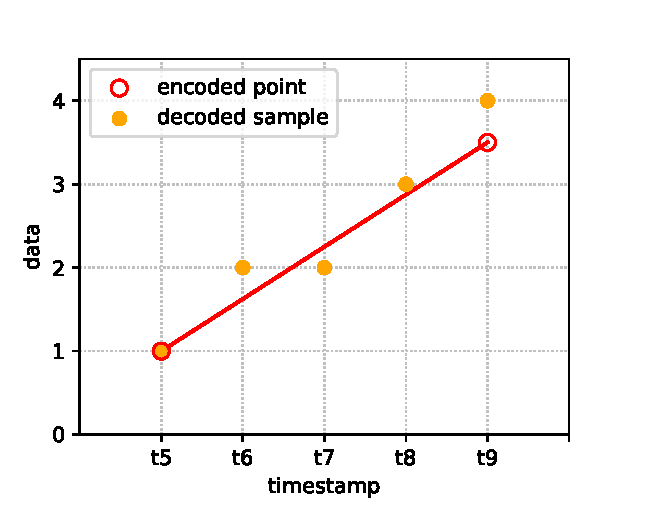
\includegraphics[width=1.2\textwidth]{chapters/3-Algorithms/examples/linear.pdf}
\vspace{-5pt}
\begin{minipage}{1.17\textwidth}
\captionof{figure}{Example of the auxiliary routine \decodeSegment\ for linear model algorithms.}
% \captionof{figure}{Example: auxiliary routine \decodeSegment\ for linear model algorithms.}
\label{example:linear}
\end{minipage}
}

\newcommand{\examplePWLH}{
\begin{figure}[h]
% \centering
\hspace{-30pt}
\begin{minipage}{.55\textwidth}
  \centering
  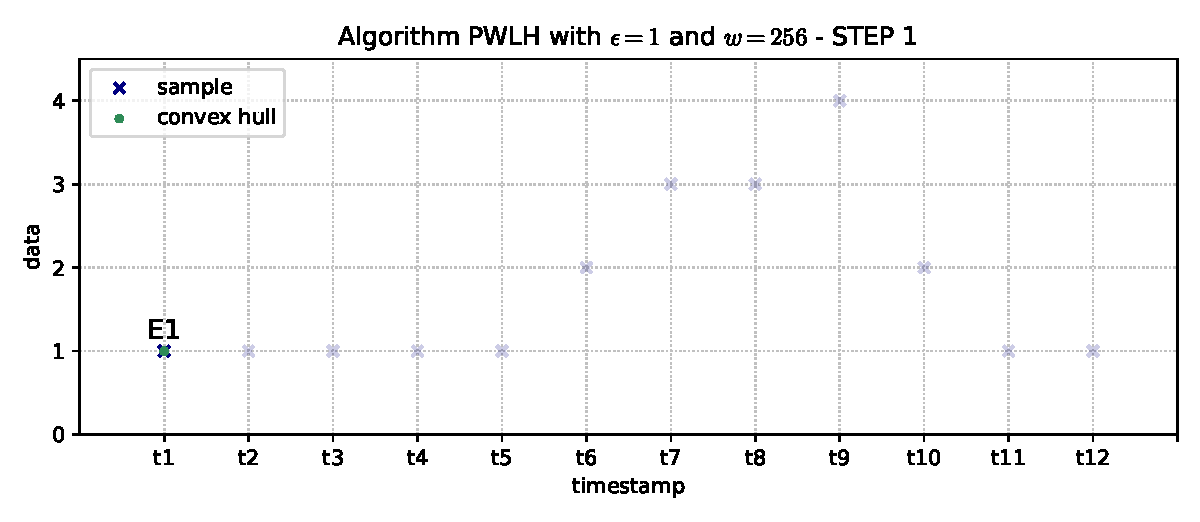
\includegraphics[clip, trim=0cm 0cm 0cm 0.9cm,width=1.0\linewidth]{chapters/3-Algorithms/examples/pwlh_intro/pwlh1.pdf}
  \vspace{-25pt}
  \captionof{figure}{\makeCaptionIntroPWLH{pwlh}{1}{1}}
  \label{example:pwlhIntro1}
\end{minipage}
\begin{minipage}{.55\textwidth}
  \centering
  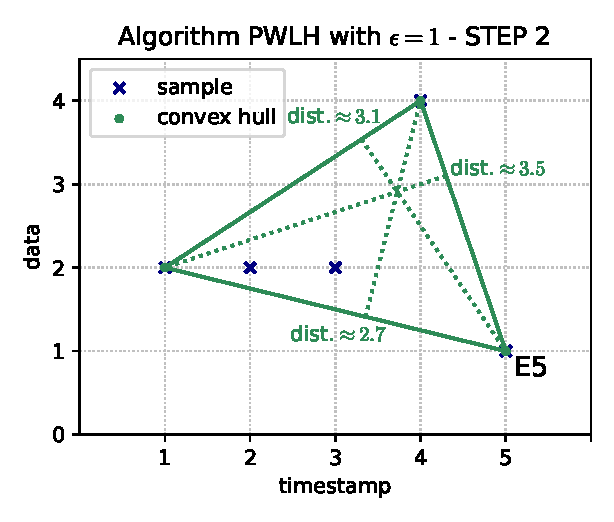
\includegraphics[clip, trim=0cm 0cm 0cm 0.9cm,width=1.0\linewidth]{chapters/3-Algorithms/examples/pwlh_intro/pwlh2.pdf}
  \vspace{-25pt}
  \captionof{figure}{\makeCaptionIntroPWLH{pwlh}{1}{2}}
  \label{example:pwlhIntro2}
\end{minipage}
\end{figure}
}

\newcommand{\exampleCA}{
\begin{figure}[h]
% \centering
\hspace{-30pt}
\begin{minipage}{.55\textwidth}
  \centering
  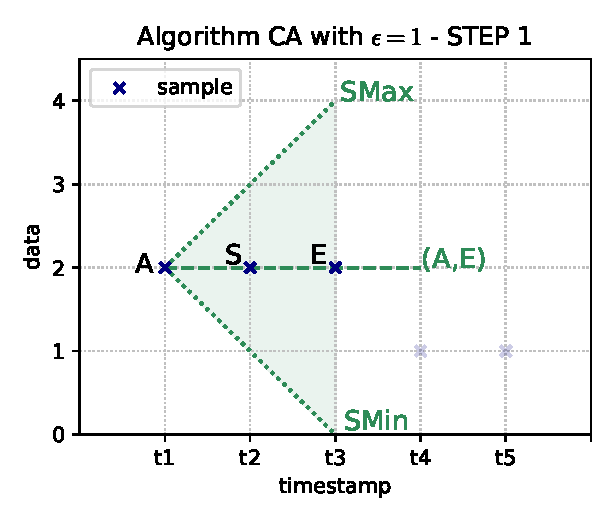
\includegraphics[clip, trim=0cm 0cm 0cm 0.9cm,width=1.0\linewidth]{chapters/3-Algorithms/examples/ca_intro/ca1.pdf}
  \vspace{-25pt}
  \captionof{figure}{\makeCaptionIntroCA{ca}{1}{1}}
  \label{example:caIntro1}
\end{minipage}%
\begin{minipage}{.55\textwidth}
  \centering
  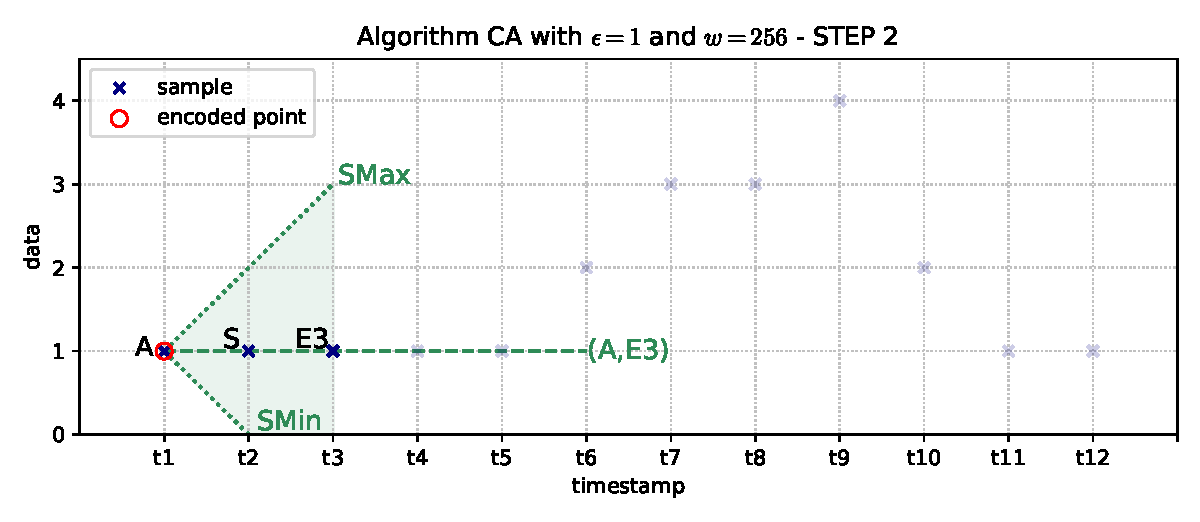
\includegraphics[clip, trim=0cm 0cm 0cm 0.9cm,width=1.0\linewidth]{chapters/3-Algorithms/examples/ca_intro/ca2.pdf}
  \vspace{-25pt}
  \captionof{figure}{\makeCaptionIntroCA{ca}{1}{2}}
  \label{example:caIntro2}
\end{minipage}
\end{figure}
}

\newcommand{\exampleSF}{
\begin{figure}[h]
% \centering
\hspace{-30pt}
\begin{minipage}{.55\textwidth}
  \centering
  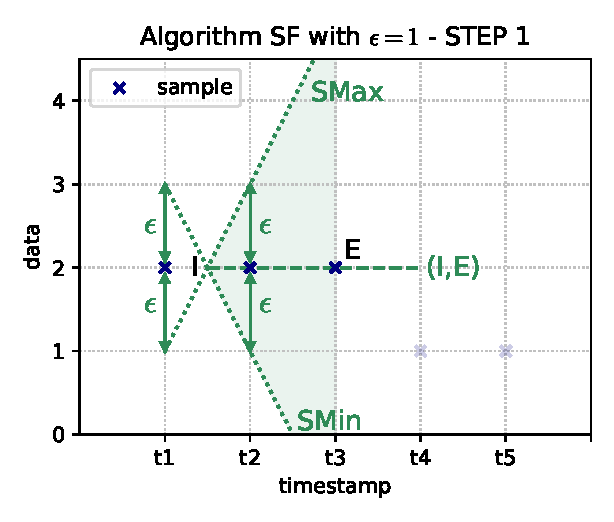
\includegraphics[clip, trim=0cm 0cm 0cm 0.9cm,width=1.0\linewidth]{chapters/3-Algorithms/examples/sf_intro/sf1.pdf}
  \vspace{-25pt}
  \captionof{figure}{\makeCaptionIntroSF{sf}{1}{1}}
  \label{example:sfIntro1}
\end{minipage}%
\begin{minipage}{.55\textwidth}
  \centering
  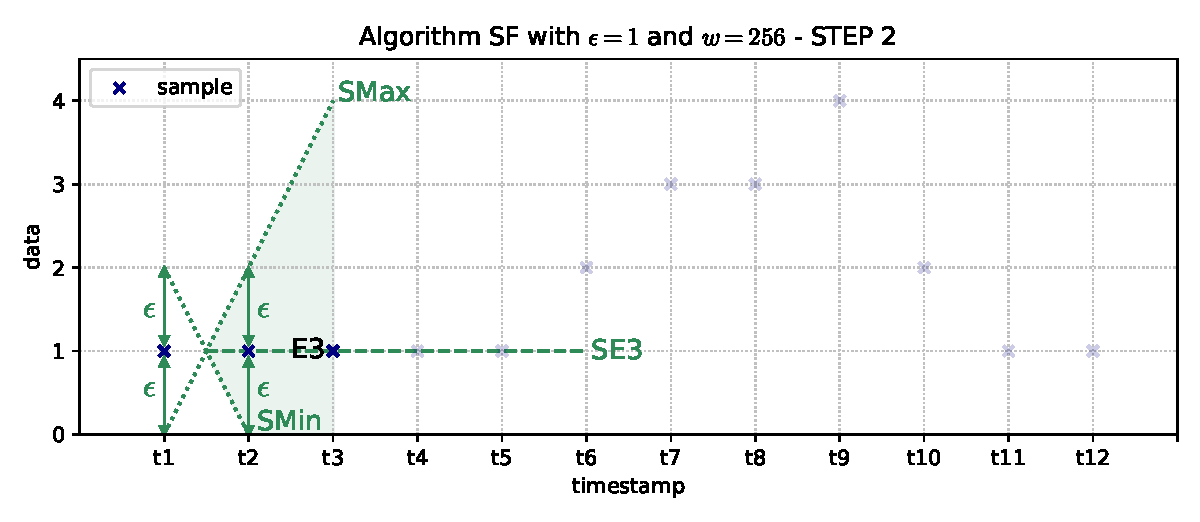
\includegraphics[clip, trim=0cm 0cm 0cm 0.9cm,width=1.0\linewidth]{chapters/3-Algorithms/examples/sf_intro/sf2.pdf}
  \vspace{-25pt}
  \captionof{figure}{\makeCaptionIntroSF{sf}{1}{2}}
  \label{example:sfIntro2}
\end{minipage}
\end{figure}
}







\newcommand{\BeCe}{B_c}


In this chapter we introduce the datasets used in our experiments. Every dataset consists of signals with one or both of the characteristics we are interested in, namely, irregular sampling rate and data gaps. In Chapter~\ref{experiments}, we present our experimental results, which make use of these datasets to analyze the compression performance of our implemented algorithm variants, which are presented in Chapter~\ref{algo}.


The datasets come from multiple sources \dataCite, each using a different data representation format. We transformed the data into a consistent, uniform format, which can be easily adapted to represent different kinds of datasets. In \textbf{Section~\ref{datasets:over}} we describe this format, including an example file that illustrates how the data is represented. In \textbf{sections~\ref{datasets:irkis}} to \textbf{\ref{datasets:wind}} we present each of the eight real-world datasets, namely, IRKIS \cite{dataset:irkis}, SST, ADCP \cite{dataset:sst1}, ElNino \cite{dataset:elnino}, Solar \cite{dataset:solar}, Hail, Tornado, and Wind \cite{dataset:spc}, laying out the source, characteristics and relevant statistics of every signal involved. Finally, in \textbf{Section~\ref{datasets:summary}} we summarize the information presented in this chapter, specifying the number of files, the number of gaps, and the data types of each dataset, as well as the measuring unit, scale, and range of each data type.


\clearpage


\section{Introduction}
\label{algo:overview}

% \vspace{-1pt}
We focus on compression algorithms for multichannel signals with irregular sampling rates and with data gaps. Signals with these characteristics are often observed in datasets gathered by WSNs, where different groups of sensors may be out of sync, some might malfunction, and errors may arise when acquiring, transmitting or storing the data. For example, this occurs in the experimental datasets presented in Chapter~\ref{datasets}. However, state-of-the-art algorithms designed for sensor data compression reported in the literature \cite{AnEva2013, Signal2016} assume, in general, that the signals have regular sampling rate and that there are no gaps in the data. Therefore, in this chapter we introduce a number of variants of state-of-the-art algorithms that we design and implement, which are adapted so they are able to encode multichannel signals with irregular sampling rates and data gaps. In Chapter~\ref{experiments} we evaluate their compression performance experimentally.


\Revisor{The original state-of-the-art algorithms considered, as well as our adapted variants, are \textit{lossy} algorithms that support near-lossless compression, which is defined as follows.}

\begin{defcion}
\Revisor{\textit{Near-lossless} compression guarantees a bounded per-sample absolute error between the decompressed and the original signals. This user-defined error threshold is specified through parameter \maxerror.}
\end{defcion}

\vspace{-5pt}
When \maxerror is zero, the compression is \textit{lossless}: the decompressed and the original signals are identical. For most algorithms we implement two variants: a \textit{masking (\maskalgo)} variant, which first encodes the position of all the data gaps, and then proceeds to encode the data values separately, and a \textit{non-masking (\NOmaskalgo)} variant, which encodes the gaps and the data values together. In both variants, regardless of the value of parameter \maxerror, the gaps in a decompressed signal match the gaps in the original signal exactly. In Section~\ref{secX:rendimiento-relativo}, we compare the compression performance of both variants, \maskalgo\ and \NOmaskalgo, for every evaluated algorithm that supports both.


Except from algorithm Base (a trivial lossless algorithm described in Section \ref{algo:base}), all our algorithm variants parse the input data into windows, which are encoded in sequence (and, in most cases, independently). The size of these windows depends on a parameter denoted $\win$. In both variants of algorithm PCA (presented in Section~\ref{algo:pca}), parameter $w$ defines a \textit{fixed window size}, while for the rest of the algorithm variants it defines a \textit{maximum window size}. More details are presented with the specific description of each algorithm, later in this chapter. In Section~\ref{secX:windows} we analyze the sensitivity of the algorithm variants to parameter $w$, in terms of their compression performance.
% Algorithm GAMPS, to be presented in Section~\ref{algo:gamps}, is an \textit{offline algorithm}: it is given all of the data to be compressed as one of its inputs. On the other hand, the rest of the algorithms are \textit{online algorithms}, since they receive the data to be compressed sequentially. 


The original algorithms and our proposed variants follow a model-based compression approach: they compress signals by exploiting \textit{temporal correlation} (i.e. correlation between signal samples taken at close times), and, in some cases, \textit{spatial correlation} (i.e. correlation between samples from different channels). They offer an efficient compression performance, as well as some data processing features, such as inferring uncertain sensor readings, detecting outliers, indexing, etc. \cite{AnEva2013}. The model-based techniques are classified into different categories, depending on the type of model: \textit{constant models} approximate signals by piecewise constant functions, \textit{linear models} use linear functions, and \textit{correlation models} simultaneously encode multiple signals exploiting temporal and spatial correlation. \Revisor{There also exist \textit{nonlinear model} algorithms, such as \textit{Chebyshev Transform} \cite{coder:chebysheb}, \textit{Discrete Cosine Transform (DCT)} and \textit{Discrete Wavelet Transform (DWT)} \cite{coder:DCT-DWT}, which approximate signals by nonlinear functions. Even though nonlinear model algorithms support lossless compression, they are mostly used for lossy compression (e.g. JPEG \cite{JPEG}, which is based on DCT, is the most popular lossy image compression standard). However, they do not support near-lossless compression and yield modest compression results on WSN data \cite{AnEva2013, Signal2016}.} In this chapter, we propose variants for eight different compression algorithms: PCA \cite{coder:pca} and APCA \cite{coder:apca} (constant model algorithms); PWLH \cite{coder:pwlh}, PWLHInt (see Subsection~\ref{algo:pwhl:int}), CA \cite{coder:ca}, SF \cite{coder:sf}, and FR \cite{coder:fr} (linear model algorithms); and GAMPS \cite{coder:gamps} (correlation model algorithm). In Section~\ref{secX:codersmask} we compare the compression performance of our adapted algorithm variants, with each other, and with the general-purpose lossless compression algorithm gzip \cite{gzip}.


In Table~\ref{algo:table:overview} we outline some characteristics of the evaluated algorithm variants. For each algorithm, the second and third columns indicate whether it supports lossless and near-lossless compression, respectively, the fourth column shows its compression model, the fifth and sixth columns indicate if the masking (\maskalgo) and non-masking (\NOmaskalgo) variants apply, respectively, and the last column specifies if the algorithm depends on a window size parameter ($w$). Algorithm Base is a trivial lossless algorithm that is used as a base ground for comparing the performance of the remaining algorithms, all of which support both lossless and near-lossless encoding.


% \vspace{+5pt}

\begin{table}[h]
\vspace{+5pt}
\begin{center}
    \begin{tabular}{| C{2.2cm} || C{1.4cm} | C{1.4cm} |  C{2cm} |  C{0.9cm} | C{0.9cm} | C{0.7cm} |}
    \hline
      \multicolumn{1}{|>{\centering\arraybackslash}m{2.2cm}||}{\textbf{Algorithm}}
    & \multicolumn{1}{>{\centering\arraybackslash}m{1.4cm}|}{\textbf{Lossless}} 
    & \multicolumn{1}{>{\centering\arraybackslash}m{1.4cm}|}{\textbf{Near-lossless}}
    & \multicolumn{1}{>{\centering\arraybackslash}m{2cm}|}{\textbf{Model}} 
    & \multicolumn{1}{>{\centering\arraybackslash}m{0.9cm}|}{\textbf{\maskalgo}} 
    & \multicolumn{1}{>{\centering\arraybackslash}m{0.9cm}|}{\textbf{\NOmaskalgo}}
    & \multicolumn{1}{>{\centering\arraybackslash}m{0.7cm}|}{\textbf{$w$}}\\
    \hline
    Base                               & x  &   & Constant     &    & x &   \\\hline
    PCA \cite{coder:pca}               & x  & x & Constant     & x  & x & x \\\hline
    APCA \cite{coder:apca}             & x  & x & Constant     & x  & x & x \\\hline
    PWLH \cite{coder:pwlh}/ PWLHInt    & x  & x & Linear       & x  & x & x \\\hline
    CA \cite{coder:ca}                 & x  & x & Linear       & x  & x & x \\\hline
    SF \cite{coder:sf}                 & x  & x & Linear       & x  &   &   \\\hline
    FR \cite{coder:fr}                 & x  & x & Linear       & x  &   & x \\\hline
    GAMPS \cite{coder:gamps}           & x  & x & Correlation  & x  & x & x \\\hline
    \toprule[0.1mm]
    \end{tabular}
    \caption{Characteristics of the evaluated coding algorithms. For each algorithm, the table shows whether it supports lossless and near-lossless compression (second and third columns, respectively), its model type (fourth column), whether the masking (\maskalgo) and non-masking (\NOmaskalgo) variants apply (fifth and sixth columns, respectively), and whether the algorithm depends on a window size parameter ($w$) (last column).}
    \label{algo:table:overview}
\end{center}
\end{table}





% \vspace{-25pt}
\clearpage
\section{General Encoding Scheme}
\label{algo:details}


\vspace{-5pt}
Figure~\ref{pseudoCodeCommon} shows a general encoding scheme used for most of the evaluated algorithms. The decoding scheme is symmetric. Constant and linear model algorithms only exploit the temporal correlation in the data, thus they iterate through the data columns and encode each independently. Since correlation models also exploit the spatial correlation (i.e. the data columns are \textit{not} encoded independently), algorithm GAMPS follows a different scheme, which we present in Section~\ref{algo:gamps}.


In Figure~\ref{pseudoCodeCommon}, the inputs for the coding routine are a CSV data file in the format presented in Chapter~\ref{datasets}, a key ($v$) that describes the algorithm variant (either \maskalgo\ or \NOmaskalgo), and the maximum error threshold (\maxerror) and window size (\win) parameters. The output is a binary file, which represents the input file encoded with a compression algorithm using the specified variant and parameters.


\vspace{+5pt}


\newcommand{\forEachColumnCoder}{\column \textnormal{ in \file.\dataColumns}}

\beginAlgorithm
\inputAndOutput{\cInputFile\\ \cInputVariant\\ \cInputThresholdOpt\\ \cInputWindowOpt}{\cOutputFileA}
Create output file \out\\
Encode an algorithm identification key, variant key \variant, and parameter \win\ (if applicable)\\
Encode the header of the input file\\
Encode the timestamp column using algorithm variant \MaskVar{APCA}\\
\If{\maskMode}{
Encode gap locations in each signal column of the input file (independently) into \out\\
}
\uIf{\textnormal{we are using a constant or linear model algorithm}}{
    Encode each signal column of the input file (independently) into \out, using the coding routine for variant \variant\ of a specific algorithm (i.e. Base, PCA, APCA, PWLH, PWLHInt, CA, SF, FR)
}
\ElseIf{\textnormal{we are using a correlation model algorithm}}{
    Encode all the signal columns of the input file into \out, using the coding routine for variant \variant\ of a specific algorithm (i.e. GAMPS)
}
\returnn \out\\
\EndPseudo{General encoding scheme for the evaluated algorithm variants.}{\label{pseudoCodeCommon}}


\newcommand{\encodedColumns}{\text{encoded\_columns}}
\newcommand{\forEachColumnDecoder}{\encodedColumn \textnormal{ in \file.\encodedColumns}}
\newcommand{\whileFileLeftToDecode}{$\notCond\ \file.\textnormal{reached\_eof?}$}

\newcommand{\decodeColParams}{\file, \out, \win, \textit{\tsColumn}}


The timestamp column, which is comprised of integers, is the first column in every CSV data file, and it is also the first column to be encoded (\Line 4). This is done using a lossless code in which every integer is encoded independently, using a fixed number of bits, $\BeCe$, which we define next.


\begin{defcion}
The number of bits $\BeCe$ required to encode a specific value of data type $z$ of a certain dataset $d$ is given by
\vspace{-5pt}
\begin{equation}
\label{eq:bece}
\BeCe(z, d) = \lceil{ \log_2 \big( \text{max}(z, d) - \text{min}(z, d) + \EneCe(z, d) \big) } \rceil,
\end{equation}
\end{defcion}
\vspace{-5pt}
where $\text{max}(z, d)$ and $\text{min}(z, d)$ are the maximum and minimum values allowed, respectively, for the data type, and $\EneCe(z, d)$ is 1 if the data type admits gaps, and 0 otherwise.


Recall, from Section~\ref{datasets:over}, that the maximum and minimum values allowed for each data type are specified in the header of the dataset CSV file, making this information known to the encoder. Also, recall that the timestamp column consists of integer values, but, in general, the rest of the columns admit both integer values and the character ``N", which represents a gap in the data. Thus, $\EneCe$ is 0 for the timestamp data type, and 1 for the rest of the data types in each dataset. Notice that $\EneCe$ is a constant that accounts for an extra symbol needed to encode a gap.


\newcommand{\gapLine}{6}
We focus on the compression of the sample columns (i.e. the rest of the columns in the data file), and do not delve into the optimization of timestamp compression, which we leave for future work. When the masking variant of the algorithm is executed, the positions of the gaps in every data column are encoded, independently for each column, in \Line \gapLine; the details are explained in Section~\ref{algo:maskmodes}. 



% \vspace{-10pt}
% \clearpage
\section{Encoding of Gaps in the Masking Variants}
\label{algo:maskmodes}


\newcommand{\xOneN}{x_1...x_n}
\newcommand{\StringSeq}{x_1...x_{i-1}}
\newcommand{\xiiminus}{p(x_i|\StringSeq)}
\newcommand{\xiiminustwo}{p(\cdot|\StringSeq)}
\vspace{-5pt}
% variant \maskalgo of an algorithm
We recall that the masking variant of an algorithm starts by losslessly encoding the position of all the gaps in the data, independently for each data column (\Line \gapLine\ in Figure \ref{pseudoCodeCommon}). We describe the position of the gaps in a column by encoding a sequence of binary symbols, $\xOneN$, each symbol $x_i$ indicating the presence ($0$) or absence ($1$) of a sample in the $i$-th timestamp of the column, in chronological order. To this end we use an arithmetic coder (AC) \cite{ac2, Cover2005}. Given a sequence of probability assignments, $\xiiminustwo$, for the symbol in position $i$ given the past symbols $x_1...x_{i-1}$, $1\leq i \leq n$, an AC generates a lossless encoding bit stream for $\xOneN$, of length $-\log P(\xOneN) + O(1)$, where $P(\xOneN)=\prod_{i=1}^{n}\xiiminus$. This code length is optimal for this probability assignment, up to an additive constant \cite{arcoding}.


\clearpage


For a sequence $x$ of independent and identically distributed random binary symbols (with unknown probability distribution), the Krichevsky–Trofimov probability assignment \cite{ktestimator}, which we define next, yields an asymptotically optimal code length for the (unknown) probability distribution, in the sense that the worst case redundancy for such code is asymptotically minimized~\cite{unicodinginfo}.


\begin{defcion}
\label{def:ktestimator}
Given a string $x$ over an alphabet $A = \{0, 1\}$, the \textit{Krichevsky–Trofimov (KT) probability assignment} assigns the following probabilities for each symbol position $i, 1\leq i \leq n$
\vspace{-2pt}
\begin{equation}
\label{eq:ktestimator}
p(0|\StringSeq) = \frac{n_0 + 1/2}{i}, \hspace{+20pt} p(1|\StringSeq) = \frac{n_1 + 1/2}{i},
\end{equation}
\end{defcion}
\vspace{-8pt}
where $n_0$ and $n_1$ denote the number of occurrences of 0 and 1 in $\StringSeq$, respectively.


\vspace{+5pt}
Analyzing the experimental datasets presented in Chapter~\ref{datasets}, we notice that the positions of the data gaps follow different patterns for different datasets, but, in general, the gaps occur in bursts. Thus, it makes sense to consider a simple binary Markov model, such as the one defined next, which captures the burstiness of data gap occurrences~\cite{markovBurst}.


\begin{table}[h]
\begin{minipage}{0.62\textwidth}
\setstretch{1.1}
% \vspace{-35pt}
The first-order Markov model has two states, $S_0$ and $S_1$, and we say that $x_i$ occurs in state $S_b$ iff the previous symbol, $x_{i-1}$, equals $b$. We arbitrarily let $S_1$ be the initial state (i.e. the state in which $x_1$ occurs). In Figure~\ref{tikz:markov} we present a diagram for this Markov model. A KT probability assignment for a first-order Markov model is obtained by applying (\ref{eq:ktestimator}) separately for the subsequence of symbols that occur in states $S_0$ and $S_1$. This is implemented by maintaining two pairs of symbol occurrence counters, $n_0$, $n_1$, one pair for each state.

\end{minipage}
\hspace{0.02\textwidth}
\begin{minipage}{0.32\textwidth}
% \vspace{+5pt}
\centering
\begin{tikzpicture}[initial text=initial]
% \node[initial, state] (A) {};
\node[state] (s0) {$S_0$};
\node[initial above, state, right=of s0] (s1) {$S_1$};
\draw[every loop]
        (s0) edge[loop left, auto=left] node {``0''} (s0)
        (s1) edge[loop right, auto=left] node {``1''} (s1)
        (s0) edge[bend left, auto=left] node {``1''} (s1)
        (s1) edge[bend left, auto=left] node {``0''} (s0);
        
\end{tikzpicture}
\captionof{figure}{Markov process diagram.}
\label{tikz:markov}

\end{minipage}
\end{table}




% \clearpage
\vspace{-10pt}
\section{Algorithm Base}
\label{algo:base}
\newcommand{\codeColumn}{$\text{code\_column}$}
\newcommand{\decodeColumn}{$\text{decode\_column}$}

\vspace{-5pt}
\Revisor{Algorithm \textit{Base} is a trivial lossless coding algorithm that yields a standard version of the uncompressed data, which serves as a base ground for comparing the performance of the rest of the algorithms. It encodes every sample independently and using the same number of bits.} 


Algorithm Base follows the general schema presented in Figure~\ref{pseudoCodeCommon}, with a specific coding routine shown in Figure~\ref{pseudoCoderBase}. This routine iterates through every entry of a column of a CSV data file. Since algorithm Base only supports variant \NOmaskalgo, these entries can be either the character ``N", which represents a gap in the data, or an integer value representing an actual data sample. Every column entry is encoded independently using $\BeCe$ bits. A special integer, \nodata, is reserved for encoding a gap. The decoding routine is symmetric to the coding routine.

% and using a fixed number of bits, which depends on the data type and the dataset. In practice, the number of bits used for encoding a data value ultimately depends on the range and accuracy of the sampling instrument used for acquiring and storing the data. 




\beginAlgorithm
\onlyInput{\columnInput\\ \outAlgo{Base}}
\ForEach{\forEachEntryCoder}{
    \eIf{\ifNoDataCoder{\entry}}{
        $\valuev = \nodata$\\
    }
    {
        $\valuev = \entry$\\
    }
    \encodeSpecific{$\valuev$}\\
}
\EndAlgorithm{Coding}{\coderBase}{\label{pseudoCoderBase}}


% \clearpage



% \newcommand{\WindowParam}{It has a window size parameter, $\win$, as defined in Section~\ref{algo:overview}, used as described below.\ }
\newcommand{\WindowParam}{}

\newcommand{\BothVariantsOne}[1]{For {#1} we define both variants, \maskalgo\ and \NOmaskalgo}
\newcommand{\BothVariantsTwo}[1]{{#1} supports both variants, \maskalgo\ and \NOmaskalgo}
\newcommand{\SingleVariant}[1]{For {#1} we define a single variant, \maskalgo}


% \vspace{-10pt}
\clearpage
\section{Algorithm PCA}
\label{algo:pca}


\vspace{-5pt}
Algorithm \textit{\PCAfull} \cite{coder:pca} is a constant model algorithm that supports lossless and near-lossless compression. \WindowParam \BothVariantsOne{PCA}.


In Figure~\ref{pseudoCoderPCAM} we show the coding routine for variant \maskalgo, in which all the column entries are integer values (the gaps are encoded separately). The column entries are parsed into consecutive non-overlapping windows of size $\win$ (\Line 1), and each of these windows is encoded independently (\Lines 3-13). 



\newcommand{\parseWindowsPCA}{Parse \column\ into consecutive non-overlapping windows of size $\win$, except possibly for the last window that may consist of fewer samples}
\newcommand{\forEachWindowPCA}{\textnormal{window in the parsing,} \window\commaa}

\beginAlgorithm
\onlyInput{\columnInput\\\cOutputFile{PCA}\\\cInputThreshold\\\cInputWindowPCA}
\parseWindowsPCA\\
\ForEach{\forEachWindowPCA}{
    \calculateMinMax, respectively\\
    \uIf{\validThreTwo}{
        \codeBit{0}\\
        \calculateMidrange\\
        \encodeSpecific{$\midrange$}
    }
    \Else{
        \codeBit{1}\\
        \ForEach{\eachValueInWindow}{
            \encodeSpecific{$\valuev$}
        }
    }
}
\EndAlgorithmVariant{Coding}{\coderPCA}{\maskalgo}{\label{pseudoCoderPCAM}}



A window in the parsing, $\window$, can be encoded in two different ways. If the difference between its maximum and minimum values is less than or equal to $2\maxerror$ (i.e. the condition in \Line 4 is satisfied), then bit 0 is output, and the value of $\midrange$ for $\window$ is encoded (\Lines 5-7). On the other hand, if the condition in \Line 4 evaluates to false, then bit 1 is output, and each of the values in $\window$ is encoded separately (\Lines 9-12). We point out that, in the former case, the absolute error between the encoded and the original values in $\window$ is guaranteed to be less than or equal to $\maxerror$, as proven by the following Lemma.


\begin{lemma}
\label{lemma:pca}
\textnormal{
Let $m, M\in \mathbb{Z}$, $\maxerror \in \mathbb{N}$, such that \validThreTwo, let \calculateMidrange, and let $y\in \mathbb{R}$, such that $m\leq y\leq M$. Then $|y-\midrange|\leq \maxerror$.
}
\end{lemma}

\newcommand{\yOne}{y’}
\begin{proof}
Assume there exists a $\yOne \in \mathbb{R}$, $m\leq \yOne\leq M$, such that $|\yOne-\midrange|> \maxerror$.

We have $|\yOne-\midrange|> \maxerror \implies 2|\yOne-\midrange|> 2\maxerror \implies |2\yOne-(m+M)|> 2\maxerror$.

If $2\yOne\geq m+M$, then $|2\yOne-(m+M)|> 2\maxerror \implies 2\yOne-(m+M)> 2\maxerror$.\\
Since $M\geq \yOne$, then $2\yOne-(m+M)> 2\maxerror \implies 2M-(m+M) = M-m > 2\maxerror$, which contradicts one of the hypothesis.

Otherwise, if $2\yOne< m+M$, then $|2\yOne-(m+M)|> 2\maxerror \implies 2\yOne-(m+M)< -2\maxerror$.\\
Since $m \leq \yOne$, then $2\yOne-(m+M)< -2\maxerror \implies 2m-(m+M)=m-M < -2\maxerror \implies M-m > 2\maxerror$, which, again, contradicts one of the hypothesis.
\end{proof}


The decoding routine for variant \maskalgo\ is shown in Figure~\ref{pseudoDecoderPCAM}. It consists of a loop that repeats until every entry in the column has been decoded, which occurs when condition in \Line 2 becomes false. Recall that the coding algorithm encodes the number of rows, as part of the header of the input file (\Line 3 in Figure~\ref{pseudoCodeCommon}), so this information is known by the decoding routine (input \colSize). Each iteration of the loop starts with the reading of a single bit from the input binary file (\Line 4). If this bit is 0, then the mid-range of an encoded window is decoded, and it is written $\sizee$ times to the decoded CSV data file (\Lines 6-7). On the other hand, if the read bit is 1, then the following process is repeated a total of $\sizee$ times: a value is decoded and written to the decoded CSV data file (\Lines 9-12).




\beginAlgorithm
\onlyInput{\dinputfile{PCA}\\\doutputfile\\\cInputWindowPCA\\\cInputColSize}
\nEqZero\\
\While{\whileColumnNotDecoded}{
    \calculateSize\\
    \decodeBit\\
    \uIf{$\bit == 0$}{
        \decodeSpecific{\midrange}\\
        Output \sizee\ copies of \midrange\ to \out
    }
    \Else{
        \RepTimes{\sizee}{
            \decodeSpecific{\valuev}\\
            Output $\valuev$ to \out
        }
    }
    \addNToSize\\
}
\EndAlgorithmVariant{Decoding}{\coderPCA}{\maskalgo}{\label{pseudoDecoderPCAM}}



\clearpage


%%%%%%%%%%%%%%%%%%%%%%%%%%%%%%%%%%%%%%%%%%%%%%%%%%%%%%%%%%%%%%%%%%%%%%%%%%%%%%%%%%%%
%%%%%%%%%%%%%%%%%%%%%%%%%%%%%%%%%%%%%%%%%%%%%%%%%%%%%%%%%%%%%%%%%%%%%%%%%%%%%%%%%%%%
%%%%%%%%%%%%%%%%%%%%%%%%%%%%%%%%%%%%%%%%%%%%%%%%%%%%%%%%%%%%%%%%%%%%%%%%%%%%%%%%%%%%


\subsection{Example}
\label{algo:pca:example}
\newcommand{\exampleRecallIrrelevant}[1]{Recall that the specific timestamp values are irrelevant for algorithm #1}


Next we present an example of the encoding of the 12 samples illustrated in Figure~\ref{example:pca:1}. \exampleRecallIrrelevant{PCA}. For this example we let the error threshold parameter ($\maxerror$) be equal to 1, and the fixed window size ($\win$) equal to 4.


\vspace{+5pt}
\exampleStepCommon{pca}{1}{\label{example:pca:1}}{Example: Signal consisting of 12 samples.}


Since there are 12 samples to encode and $\win=4$, three windows are encoded independently, each consisting of exactly four samples. The first window includes the first four samples, which are all equal to 1, so in this case the condition in \Line 4 of the coding routine is satisfied. Therefore, \Lines 5-7 are executed, which encode a single value, \midrange, as a representation of the four samples in the window. For this first window, \midrange\ equals 1. Figure~\ref{example:pca:2} shows this step in the graph. Notice that, since all the values in the window are equal, the condition in \Line 4 would be satisfied regardless of the value of parameter $\maxerror$.


\vspace{+5pt}
\exampleStepPCA{pca}{2}{\label{example:pca:2}}{1}


\clearpage


The second window is comprised of the next four samples, i.e. $[1, 2, 3, 3]$. Again, the condition in \Line 4 is satisfied, because we have $|3 - 1| \leq 2*1$, but in this case \midrange\ equals 2, so these four samples are described through the encoding of a single value, 2. This step is shown in Figure~\ref{example:pca:3}.


\exampleStepPCA{pca}{3}{\label{example:pca:3}}{2}


The third and last window consists of the last four samples, i.e. $[4, 2, 1, 1]$. In this case, the condition in \Line 4 evaluates to false, so \Lines 9-12 are executed, which encode each sample value separately. This last step is shown in Figure~\ref{example:pca:4}.


\vspace{+5pt}
\exampleStepPCA{pca}{4}{\label{example:pca:4}}{3}


This simple example fairly represents every scenario that may arise during the encoding process. Since the threshold condition holds for the first two windows, both are encoded with exactly the same number of bits, i.e. $1+\BeCe$. On the other hand, since the threshold condition does not hold for the last window, it is encoded with $1 + w*\BeCe$ bits. Thus, windows consisting of adjacent samples are encoded using less bits. This example illustrates why algorithm PCA is expected to achieve better compression performances on slowly varying signals rather than rough signals.


%%%%%%%%%%%%%%%%%%%%%%%%%%%%%%%%%%%%%%%%%%%%%%%%%%%%%%%%%%%%%%%%%%%%%%%%%%%%%%%%%%%%
%%%%%%%%%%%%%%%%%%%%%%%%%%%%%%%%%%%%%%%%%%%%%%%%%%%%%%%%%%%%%%%%%%%%%%%%%%%%%%%%%%%%
%%%%%%%%%%%%%%%%%%%%%%%%%%%%%%%%%%%%%%%%%%%%%%%%%%%%%%%%%%%%%%%%%%%%%%%%%%%%%%%%%%%%


\subsection{Non-Masking (\NOmaskalgo)\ Variant}
\label{algo:pca:nmvariant}


In Figure~\ref{pseudoCoderPCANM} we show the coding routine for variant \NOmaskalgo\ of algorithm PCA. In this case, the column entries may be not only integers representing sample values, but also the character \noData, which represents a gap in the data. As in variant \maskalgo, after parsing the column entries into consecutive non-overlapping windows of size $\win$ (\Line 1), each of these windows is encoded independently (\Lines 3-23). However, since not every entry in a window is guaranteed to be an integer, we consider additional scenarios when encoding a window.




\beginAlgorithm
\onlyInput{\columnInput\\\cOutputFile{PCA}\\\cInputThreshold\\\cInputWindowPCA}
Parse \column\ into consecutive non-overlapping windows of size $\win$, except possibly for the last window that may consist of fewer samples\\
\ForEach{\forEachWindowPCA}{
    \uIf{\textnormal{every entry in \window\ is equal to \noData}}{
        \codeBit{0}\\
        \encodeSpecific{$\nodata$}\\
    }
    \Else{
        \calculateMinMax, resp.\\
        \uIf{\textnormal{every entry in \window\ is different from \noData}\andd \validThreTwo}{
            \codeBit{0}\\
            \calculateMidrangeTwo\\
            \encodeSpecific{$\midrange$}
        }
        \Else{
            \codeBit{1}\\
            \ForEach{\eachEntryInWindow}{
                \eIf{\ifNoDataCoder{\entry}}{
                    $\valuev = \nodata$\\
                }
                {
                    $\valuev = \entry$\\
                }
                \encodeSpecific{$\valuev$}\\
            }
        }
    }
}
\EndAlgorithmVariant{Coding}{\coderPCA}{\NOmaskalgo}{\label{pseudoCoderPCANM}}



A window $\window$ can be encoded in three different ways. If every entry in $\window$ represents a gap in the data (i.e. the condition in \Line 3 is satisfied), then bit 0 is output, and the special integer \nodata\ is encoded (\Lines 4-5). If every entry in $\window$ represents a sample value, and the difference between its maximum and minimum values is less than or equal to $2\maxerror$ (i.e. the condition in \Line 8 is satisfied), then bit 0 is output, and the value of $\midrange$ for $\window$ is encoded (\Lines 9-11). In this case, due to Lemma~\ref{lemma:pca}, the absolute error between the encoded and the original values in $\window$ is guaranteed to not be greater than \maxerror. In every other case, bit 1 is output, and each of the entries in $\window$ is encoded separately (\Lines 13-21), using \nodata\ for encoding a gap. Notice that in the first two cases the window is encoded with the same number of bits, i.e. $1+\BeCe$, while in the last case the window is encoded with $1 + w*\BeCe$ bits.


The decoding routine for variant \NOmaskalgo\ is quite similar to the decoding routine for variant \maskalgo, presented in Figure~\ref{pseudoDecoderPCAM}, the only difference being that, in \Lines 6-7 and 10-11, when \nodata\ is decoded, a character \noData\ is written to the decoded CSV data file.



\clearpage

\section{Algorithm APCA}
\label{algo:apca}


Algorithm APCA \cite{coder:apca}, also known as Adaptive Piecewise Constant Approximation, is a Constant model algorithm that supports lossless and near-lossless compression. As its name suggests, it operates similarly to algorithm PCA, the difference being that in APCA the size of the blocks in which the data are separately processed and encoded is not fixed, but variable. In this case, the window size parameter ($\win$) establishes a maximum block size for the algorithm. APCA supports both variants, \maskalgo\ and \NOmaskalgo.


In Figure~\ref{pseudoCoderAPCAM} we show the coding routine for variant \maskalgo, in which all the column entries are integer values (the gaps are encoded separately). It consists of a loop that iterates over all column entries. The algorithm maintains a window of consecutive samples, $\window$, which is initially empty (line 1). In each iteration, the addition of an entry to the window is considered (lines 3-9). If the new entry makes the window violate the error threshold constraint (i.e. the absolute difference between its maximum and minimum values is greater than $2*\maxerror$), or the window size greater than $\win$, then the window is encoded, and a new empty window is created (lines 6-7). In any case, the current entry is added to $\window$ (line 9), and is eventually encoded. In particular, if the loop ends and $\window$ is not empty, it is encoded in line 12. 




\beginAlgorithm
\onlyInput{\columnInput\\\outVarM{APCA}\\\cInputThreshold\\\cInputWindowAPCA}
\createWindowOne\\
\ForEach{\forEachEntryCoder}{
    \calculateMinMaxAPCA\\
    \If{\NOTvalidThreThree\ \orr \windowFull}{
        \encodeWindowAPCA\\
        \createWindowTwo\\
    }
    \AddEntry\\
}
\If{\window \textnormal{ is not empty}}{
  \encodeWindowAPCA\\
}
\EndAlgorithmVariantM{Coding}{\coderAPCA}{\label{pseudoCoderAPCAM}}




\vspace{+2pt}
The routine called for encoding a window (lines 6 and 12), EncodeWindow, is shown in Figure~\ref{apcaWindowM}. Observe that every window is encoded with the same number of bits, i.e. $\logWinSize\ +\ \colTotBits$, where $\logWinSize$ bits are used for encoding its size, and $\colTotBits$ bits are used for encoding its mid-range.
\vspace{+3pt}




\beginAlgorithm
\onlyInput{\windowInput\\\cOutputFile{APCA}\\\cInputWindowAPCA}
\encodeWindowSizee\\
\calculateMinMax, respectively\\
\calculateMidrangeTwo\\
\encodeSpecific{$\midrange$}\\
\EndPseudo{EncodeWindow routine for algorithm \coderAPCA.}{\label{apcaWindowM}}



\clearpage


The decoding routine for variant \maskalgo\ is shown in Figure~\ref{pseudoDecoderAPCAM}. It consists of a loop that keeps running until every entry in the column has been decoded, which occurs when condition in line 2 becomes false. The decoding loop is fairly simple. First, both the window size, \sizee, and its mid-range value are decoded (lines 2-3). Then, the mid-range value is written \sizee\ times to the decoded csv data file (line~5).




\beginAlgorithm
\onlyInput{\inVarM{APCA}\\\doutputfile\\\cInputWindowAPCA\\\cInputColSize}
\nEqZero\\
\While{\whileColumnNotDecoded}{
    \decodeWindowwSize\\
    \decodeSpecific{\midrange}\\
    Output \sizee\ copies of \midrange\ to \out\\
    \addNToSize\\
}
\EndAlgorithmVariantM{Decoding}{\coderAPCA}{\label{pseudoDecoderAPCAM}}



%%%%%%%%%%%%%%%%%%%%%%%%%%%%%%%%%%%%%%%%%%%%%%%%%%%%%%%%%%%%%%%%%%%%%%%%%%%%%%%%%%%%
%%%%%%%%%%%%%%%%%%%%%%%%%%%%%%%%%%%%%%%%%%%%%%%%%%%%%%%%%%%%%%%%%%%%%%%%%%%%%%%%%%%%
%%%%%%%%%%%%%%%%%%%%%%%%%%%%%%%%%%%%%%%%%%%%%%%%%%%%%%%%%%%%%%%%%%%%%%%%%%%%%%%%%%%%


\subsection{Example}
\label{algo:apca:example}


Next we present an example of the encoding of 12 samples illustrated in Figure~\ref{example:pca:1}. Notice that the specific timestamp values are irrelevant for this algorithm. In this example we use algorithm APCA with an error threshold parameter ($\maxerror$) equal to 1, and a maximum window size ($\win$) equal to 256. 


The condition in line 5 of the coding routine evaluates to false in the first eight iterations, so those samples, $[1, 1, 1, 1, 1, 2, 3, 3]$, are added to the first window. The sample processed in the 9th iteration is 4, whose addition to the window would violate the error threshold constraint, because we have $|4 - 1| > 2*1$. Therefore, the window is encoded, which requires $\logWinSize = \logWinSizeOpt{256}=8$ bits for encoding its size (i.e. 8), and $\colTotBits$ for encoding its mid-range (i.e. 2), and the sample value 4 is added to a new empty window. This step is shown in Figure~\ref{example:apca:1}.


\exampleStep{apca}{1}{\label{example:apca:1}}{Algorithm APCA example. Step 1.}


For the second window, the condition in line 5 evaluates to false in the 10th iteration. However, the error threshold constraint is violated in the 11th iteration, for the sample value 1. The second window, $[4, 2]$, is encoded with size 2 and mid-range 3, and the sample value 1 is added to a new empty window. This step is shown in Figure~\ref{example:apca:2}.


\exampleStep{apca}{2}{\label{example:apca:2}}{Algorithm APCA example. Step 2.}


For the third window, the condition in line 5 evaluates to false in the 12th and last iteration. This window, which is equal to $[1, 1]$, is encoded after executing the last iteration, in line 12. In this case, the window size is 2 and its mid-range is 1. This last step is shown in Figure~\ref{example:apca:3}.


\exampleStep{apca}{3}{\label{example:apca:3}}{Algorithm APCA example. Step 3.}


We point out that the three windows encoded in this example use exactly the same amount of bits. However, the first window consists of eight samples, while the last two consist of only two samples. Therefore, the first window achieves a better compression ratio (more samples encoded per bit). This example illustrates why algorithm APCA is expected to achieve better compression performances on slowly varying signals rather than rough signals.


%%%%%%%%%%%%%%%%%%%%%%%%%%%%%%%%%%%%%%%%%%%%%%%%%%%%%%%%%%%%%%%%%%%%%%%%%%%%%%%%%%%%
%%%%%%%%%%%%%%%%%%%%%%%%%%%%%%%%%%%%%%%%%%%%%%%%%%%%%%%%%%%%%%%%%%%%%%%%%%%%%%%%%%%%
%%%%%%%%%%%%%%%%%%%%%%%%%%%%%%%%%%%%%%%%%%%%%%%%%%%%%%%%%%%%%%%%%%%%%%%%%%%%%%%%%%%%


\clearpage
\subsection{Non-masking (\NOmaskalgo)\ variant}
\label{algo:apca:nmvariant}


The coding and decoding routines for variant \NOmaskalgo\ of algorithm APCA are similar to their variant \maskalgo\ counterparts, the difference being that the former routines are able to handle both sample values and gaps. Recall that in the coding routine for variant \maskalgo, a window is encoded when adding a new entry would make it violate the error threshold constraint or the window size restriction (line 5 in Figure~\ref{pseudoCoderAPCAM}). In the coding routine for variant \NOmaskalgo, a window must also be encoded if the newest entry is character \noData\ (gap in the data) and the other entries in the window are integers (sample values), or vice versa. A window that consists of gaps is encoded with the same number of bits as a window that consists of integers, i.e. $\logWinSize\ +\ \colTotBits$, where $\logWinSize$ bits are used for encoding its size, and $\colTotBits$ bits are used for encoding the special integer \nodata.



\section{Encoding Scheme for Linear Model Algorithms}
\label{algo:decolinear}


In the following four sections we present the evaluated linear model algorithms, i.e. PWLH, PWLHInt, CA, SF and FR. As we recall from Section~\ref{algo:overview}, these type of algorithms approximate signals using linear functions. Even though the encoding scheme varies among algorithms, it always requires encoding a sequence of line segments in the two-dimensional Euclidean space. Each line segment represents a sequence of consecutive samples, with x-axis and y-axis corresponding to timestamps and sample values, respectively.


A linear model encoding algorithm operates by successively encoding endpoints of segments, which span samples whose distance to the segment along the y-axis does not exceeds the prescribed error threshold parameter ($\maxerror$). The decoder, in turn, sequentially decodes the endpoints of each segment and linearly interpolates the intermediate samples. In Figure~\ref{pseudoDecoLinear} we present the auxiliary routine \decodeSegment, which performs this interpolation; it is used by the decoding routine of all linear model algorithms. Its inputs are the timestamp column (recall that this column is encoded first and, thus, it is available to the decoder when decoding sample columns), and a pair of timestamps and sample values, which correspond to the coordinates of a segment's endpoints (\Line~1). The output is a list consisting of the sample values that are decoded from said segment.




\beginAlgorithm
\inputAndOutput{\inputTSCol\\\inputTSO\\\inputTSN\\\inputSO\\\inputSN}{\outputDecoded}
Let \segment\ be the line segment whose endpoints coordinates are (\tsO,\sO) and (\tsN,\sN)\\
Create an empty list, \decodedSamples\\
\ForEach{\forEachTS \textnormal{ such that} \ifDecoLinear \commaa}{
    Let \sI\ be the sample value obtained when substituting the x-coordinate in the \segment\ equation by \tsI, and rounding the result to the nearest integer\\
    \AddEntryLinear
}
% \returnn \decodedSamples
\EndPseudo{Auxiliary routine \decodeSegment for linear model algorithms.}{\label{pseudoDecoLinear}}




\clearpage


For most algorithms, both the x-coordinates and the y-coordinates of the endpoints are encoded as integers, the exceptions being algorithm PWLH, presented in Section~\ref{algo:pwlh}, which encodes the y-coordinates as floats, and algorithm SF, presented in Section~\ref{algo:sf}, which encodes the coordinates of both axes as floats.


Next, we present an example that illustrates the working of the auxiliary routine \decodeSegment. The inputs are represented in Figure~\ref{example:linear}: the coordinates of the encoded segment endpoints

\vspace{-12pt}
\begin{table}[h]
\begin{minipage}{0.45\textwidth}
\setstretch{1.1}
% \vspace{-35pt}
are $(t_5,1)$ and $(t_9,3.5)$, while the timestamp column is equal to $[t_1,...,t_N]$, where $N \geq 9$. The segment defined in \Line 1 of the routine is colored red. After creating the empty list of decoded samples (\Line 2), a loop iterates over every timestamp $t_i$, $t_5 \leq t_i \leq t_9$, in the column, it decodes the corresponding sample value $s_i$ (\Line 4), and adds it to the list (\Line 5). Given timestamp $t_i$, sample value $s_i$ is obtained by taking the equation of the segment and substituting $t_i$ for the x-coordinate, then rounding the result to the nearest integer. In Figure~\ref{example:linear}, the decoded sample values, $s_i$, $5 \leq i \leq 9$, are colored in orange. They are equal to $[1, 2, 2, 3, 4]$, which is the list output by the routine \decodeSegment in this example.
\end{minipage}
\hspace{0.02\textwidth}
\begin{minipage}{0.49\textwidth}
\examplelinear
\end{minipage}
\end{table}




\section{Algorithms PWLH and PWLHInt}
\label{algo:pwlh}
\newcommand{\EncodeWindow}{EncodeWindow}


Algorithm \textit{\PWLHfull} \cite{coder:pwlh} is a linear model algorithm that supports lossless and near-lossless compression. \WindowParam \BothVariantsOne{PWLH}. We also define algorithm \textit{PWLHInt} by introducing minor design changes to algorithm PWLH. The description in the current section applies to both PWLH and PWLHInt, except for the specific differences that are pointed out in Subsection~\ref{algo:pwhl:int}.


PWLH is a linear model algorithm, so its encoding process involves the encoding of a sequence of line segments. In Figure~\ref{pseudoCoderPWLHM} we present the coding routine for variant \maskalgo. It consists of a loop that iterates over all column entries, which are always integer values (the gaps are encoded separately). The algorithm maintains a window of consecutive sample points, $\window$, which is initially empty (\Line~1). In each iteration, the addition of a new incoming point, \incoming, to the window is considered (\Lines~3-16). Notice that \incoming, defined in \Lines~3-4, is a sample point (recall definition in Section~\ref{algo:decolinear}): its y-coordinate is an integer sample value, and its x-coordinate is the timestamp (obtained from the timestamp column) for said sample. We point out that in algorithm PWLH, as well as in every evaluated linear model algorithm, windows consist of sample points, while in the constant and correlation model algorithms, windows consist of integer values corresponding to column entries.


\clearpage




\beginAlgorithm
\onlyInput{\columnInput\\\outVarM{PWLH}\\\cInputThreshold\\\cInputWindowAPCA\\\inputTSCol}
\createWindowOne\\
\ForEach{\forEachEntryCoder}{
    \obtainTS\\
    \letPoint\\
    \If{\firstIteratCA}{
        \appendIncoming\\
        \continueAlgo\\
    }
    Let \PWLHSet\ be the set of points in the \extendedWin\\
    Let \hull\ be the convex hull of \PWLHSet\\
    Let \validHull\ be true iff \hull\ satisfies the valid hull condition, defined in \ref{def:validHull}, for \maxerror\\
    \If{\nott\,\validHull \orr \windowFull\ }{
        \encodeWindowPWLH\\
        \createWindowTwo\\
    }
    \appendIncoming\\
}
\If{\winNoEmpty}{
    \encodeLastWindowPWLH\\
}
\EndAlgorithmVariantM{Coding}{\coderPWLH}{\label{pseudoCoderPWLHM}}



The incoming points obtained in the subsequent iterations are parsed into consecutive windows of variable size (up to a maximum size $\win$), such that the set of points in a certain window satisfy the \textit{valid hull condition}, defined in the next paragraph. If the set of points in a window satisfies the valid hull condition, the absolute error between the encoded and the original samples is guaranteed to be less than or equal to \maxerror. To compute the convex hull we apply Graham's Scan algorithm \cite{GrahamAlgo}. Since the points are already sorted by their respective x-coordinates, the sorting step in the algorithm is eliminated, and the time complexity to build and update the convex hull is $O(n)$ instead of $O(n \log n)$ \cite{AnEva2013}.


\vspace{+5pt}
\begin{defcion}
\label{def:validHull}
Let \PWLHSet\ be a set of points, with $|\PWLHSet|>1$, and let \hull\ be the convex hull of \PWLHSet. \hull\ satisfies the \textit{valid hull condition} for a maximum error threshold \maxerror, iff there exists an edge line in the boundary of \hull, for which the maximum Euclidean distance from any of the points in \hull\ to said edge line is less than or equal to $2\maxerror$.
\end{defcion}

\newcommand{\condLinePWLH}{\Line 12}
In figures \ref{example:pwlhIntro1} and \ref{example:pwlhIntro2} we present an example that illustrates how the valid hull condition is checked in the coding routine of Figure~\ref{pseudoCoderPWLHM}. In Figure~\ref{example:pwlhIntro1}, set \PWLHSet, which is defined in \Line 9, contains the three points in $\window$, plus the incoming point, \incomingP{4}. In this case, the convex hull of \PWLHSet, \hull, satisfies the valid hull condition for $\maxerror = 1$, since the maximum distance from any of its points to the upper edge line of its boundary is approximately 1.1, which is less than $2\maxerror = 2$. Therefore, the condition in \condLinePWLH\ evaluates to false (we assume that $|\window|<\win$), and \incomingP{4} is added to $\window$ (\Line 16). In the next step, presented in Figure~\ref{example:pwlhIntro2}, set \PWLHSet\ contains the four points in $\window$, plus \incomingP{5}. In this case, \hull\ does not satisfy the valid hull condition, since for each of the three edge lines in its boundary, there exists a point in \hull\ such that its distance to the edge line is greater than~$2\maxerror$. Therefore, the condition in \condLinePWLH\ is satisfied, so $\window$ is encoded (\Line 13), emptied (\Line 14) and added \incomingP{5} (\Line 16).


\vspace{+5pt}
\examplePWLH


\vspace{+5pt}
A window is encoded via the auxiliary routine \EncodeWindow, shown in Figure~\ref{pwlhWindowM}. This method first encodes the window size using $\logWinSize$ bits (\Line 1), then selects the segment that minimizes the \textit{mean square error (MSE)} for the points in the window, taken among all the segments for which the x-coordinates of the first and last endpoints match the x-coordinates of the first and last points in the window, respectively (\Lines 2-3). Notice that the y-coordinates of the two endpoints of this segment are float values, which may not match the value of any column entry, and might even be out of the range specified in the dataset CSV file for the corresponding data type. Finally, in \Lines 5-6, both y-coordinates are encoded as floats, using 32 bits. Recall that the coding algorithm encodes the timestamp column, with the respective x-coordinates, first. Thus, the decoding routine is able to decode both coordinates of each endpoint.





\beginAlgorithm
\onlyInput{\windowInput\\\outVarM{PWLH}\\\cInputWindowAPCA\\\inputTSCol}
\encodeWindowSizee\\
Let \segment\ be the line segment that minimizes the MSE for the points in $\window$\\
Let \sO\ and \sN\ be the y-coordinates of the endpoints of \segment\\
\codeFloat{\sO}\\
\codeFloat{\sN}
\EndAuxVarM{\EncodeWindowCA}{PWLH}{\label{pwlhWindowM}}



We point out that calculating the segment that minimizes the MSE for a set of points is computationally more expensive than checking the valid hull condition \cite{AnEva2013}. This is the reason why the valid hull condition is checked in every iteration, when deciding whether or not a point should be added to the window, while the segment that minimizes the MSE is only computed for the points in a complete window.


In the coding routine presented in Figure~\ref{pseudoCoderPWLHM}, if $\window$ is not empty after executing the last iteration of the loop, it is encoded in \Line 19, via the auxiliary routine \EncodeLastWindowPWLH, shown in Figure~\ref{pwlhLastWindowM}. If $\window$ consists of a single point, its size is encoded using $\logWinSize$ bits, and the y-coordinate of the point is encoded using \tobitexp. On the other hand, if $\window$ consists of multiple points, it is encoded in the same way as the previous windows, i.e. via the auxiliary routine \EncodeWindow, shown in Figure~\ref{pwlhWindowM}.





\beginAlgorithm
\onlyInput{\windowInput\\\outVarM{PWLH}\\\cInputWindowAPCA\\\inputTSCol}
\uIf{$|\window| == 1$}{
\encodeWindowSizeeOne\\
\encodeSpecific{the y-coordinate of the single point in \window}\\
}
\Else{
\encodeWindowPWLH
}
\EndAuxVarM{\EncodeLastWindowPWLH}{PWLH}{\label{pwlhLastWindowM}}




\vspace{+5pt}
The decoding routine for variant \maskalgo\ is shown in Figure~\ref{pseudoDecoderPWLHM}. It consists of a loop that repeats until every entry in the column has been decoded, which occurs when condition in \Line 2 becomes false. Recall that the coding algorithm encodes the timestamp column first (\Line \gapLine\ in Figure~\ref{pseudoCodeCommon}), so the timestamps are known to the decoding routine (input \tscol). Each iteration of the loop starts with the decoding of the window size (\Line 3). If the window size is greater than 1, then the points in the window are modeled by a line segment. In this case, the decoding routine decodes the float representation of the y-coordinates of the segment endpoints (\Lines 5-6), obtains the timestamps corresponding to their x-coordinates (\Line 7), and calls the auxiliary routine \decodeSegment with those inputs (\Line 8). As we recall from Figure~\ref{pseudoDecoLinear}, routine \decodeSegment returns a list consisting of the sample values that are decoded from the segment, which are then written in the decoded CSV data file (\Lines 9-11). Notice that, even though inputs \sO\ and \sN\ are floats, \decodeSegment returns a list of integers. When the window size is equal to 1, a value is decoded (using $\BeCe$ bits) and written to the decoded file (\Lines 13-14).




\newcommand{\forEachEntryDecoded}{\textnormal{sample in \decodedSamplesTwo, \valuevP,}}

\beginAlgorithm
\onlyInput{\inVarM{PWLH}\\\doutputfile\\\cInputWindowAPCA\\\cInputColSize\\\inputTSCol}
\nEqZero\\
\While{\whileColumnNotDecoded}{
    \decodeWindowwSize\\
    \uIf{$\sizee > 1$}{
        \decodeFloat{\sO}\\
        \decodeFloat{\sN}\\
        Obtain timestamps for the endpoints of the segment, \tsO\ and \tsN, from \tscol\\
        $\decodedSamplesTwo =  \decodeSegment$(\tscol, \tsO, \tsN, \sO, \sN) // routine in Figure~\ref{pseudoDecoLinear}\\
        \ForEach{\forEachEntryDecoded}{
            Output $\valuev$ to \out
        }
    }
    \Else{
        \decodeSpecific{\valuev}\\
        Output $\valuev$ to \out
    }
    \addNToSize\\
}
\EndAlgorithmVariantM{Decoding}{\coderPWLH}{\label{pseudoDecoderPWLHM}}





%%%%%%%%%%%%%%%%%%%%%%%%%%%%%%%%%%%%%%%%%%%%%%%%%%%%%%%%%%%%%%%%%%%%%%%%%%%%%%%%%%%%
%%%%%%%%%%%%%%%%%%%%%%%%%%%%%%%%%%%%%%%%%%%%%%%%%%%%%%%%%%%%%%%%%%%%%%%%%%%%%%%%%%%%
%%%%%%%%%%%%%%%%%%%%%%%%%%%%%%%%%%%%%%%%%%%%%%%%%%%%%%%%%%%%%%%%%%%%%%%%%%%%%%%%%%%%


\clearpage


\subsection{Example}
\label{algo:pwlh:example}
\newcommand{\exampleIntro}[1]{\exampleIntroFirst{#1}. For this example we let the interval between consecutive timestamps be equal to 60, the error threshold parameter ($\maxerror$) equal to 1, and the maximum window size ($\win$) equal to 256.}


\exampleIntro{\ref{example:pwlh:1}}


Since there are only 12 samples to encode, no window in this example can reach the maximum size (256). Therefore, a window is only encoded when the convex hull, defined in \Line 10 of the coding routine, violates the valid hull condition defined in \Line 11. The first iteration is the only one in which the condition in \Line 5 is satisfied, so the algorithm just adds the first incoming point, \incomingP{1}, to the window (\Line 6). Figure~\ref{example:pwlh:1} shows this step in the graph. Observe that, besides the sample points, the convex hull for the current window is also shown.


\vspace{+5pt}
\exampleStep{pwlh}{1}{\label{example:pwlh:1}}{1}


\newcommand{\widthh}{\textit{distance}}
In the second iteration, the boundary of the convex hull that includes incoming point \incomingP{2} consists of a single line segment, where the maximum distance from either point to the line is zero, so the valid hull condition is satisfied, and \incomingP{2} is added to the window. This step is shown in Figure~\ref{example:pwlh:2}.


\exampleStep{pwlh}{2}{\label{example:pwlh:2}}{2}


\clearpage


The following three sample values are also equal to 1. The convex hull that includes the respective incoming points still consists of a single line segment, so these points are also added to the window. This step is shown in Figure~\ref{example:pwlh:3}.


\exampleStep{pwlh}{3}{\label{example:pwlh:3}}{3}


In the 6th iteration, sample value 2 is considered. The updated convex hull, whose boundary now consists of three edges, is shown in Figure~\ref{example:pwlh:4}. In this case, the maximum distance between the upper edge in its boundary and any of its points is approximately $0.8$, which is less than $2\maxerror=2$. Therefore, the valid hull condition is still satisfied, and \incomingP{6} is added to the window.


\vspace{+5pt}
\exampleStep{pwlh}{4}{\label{example:pwlh:4}}{4}


\clearpage


The following three iterations are similar to the previous one. In every case, the convex hull is updated, and, even though the maximum distance between the upper edge in its boundary and any of its points increases, it is never greater than $2\maxerror$, so the three incoming points are added to the window. These steps are shown in figures~\ref{example:pwlh:5}, \ref{example:pwlh:6} and \ref{example:pwlh:7}. 

\vspace{+5pt}
\exampleStepMany{pwlh}{5}{\label{example:pwlh:5}}{5}

\vspace{-15pt}
\exampleStepMany{pwlh}{6}{\label{example:pwlh:6}}{6}

\vspace{-15pt}
\exampleStepMany{pwlh}{7}{\label{example:pwlh:7}}{7}

\clearpage


Eventually, in the 10th iteration, sample value 2 is considered. In the updated convex hull, which is shown in Figure~\ref{example:pwlh:8}, for the first time the valid hull condition is not satisfied, i.e. \validHull\ in \Line 11 becomes false. Observe that, for each of the four edges in the boundary of the convex hull, there exists a point in the hull such that its distance to the edge line is greater than $2\maxerror$. 


\vspace{+5pt}
\exampleStep{pwlh}{8}{\label{example:pwlh:8}}{8}


Since the condition in \condLinePWLH\ becomes true, the window is encoded via the auxiliary routine \EncodeWindow\ (\Line 13), and the window is emptied and added \incomingP{10} (\Lines 14 and 16). Routine \EncodeWindow\ models the points in the window through the line segment that minimizes the MSE for said points (recall Figure~\ref{pwlhWindowM}). This segment and its two encoded endpoints are shown in Figure~\ref{example:pwlh:9}. Encoding the window requires $\logWinSize = \logWinSizeOpt{256}=8$ bits for encoding its size (i.e. 9), and 32 bits for encoding each of the float values corresponding to the y-coordinates of the segment endpoints.


\vspace{+5pt}
\exampleStep{pwlh}{9}{\label{example:pwlh:9}}{9}


\clearpage


In the last two iterations of the coding routine, which correspond to the last two samples, the valid hull condition is not violated. Therefore, after executing the last iteration, $\window$ includes three points, which are encoded via the auxiliary routine \EncodeLastWindowPWLH\ (\Line 19). The associated segment, with its two encoded endpoints, is shown in Figure~\ref{example:pwlh:10}. In this figure, we also display the values of the decoded samples, which are the values that the decoding routine, shown in Figure~\ref{pseudoDecoderPWLHM}, writes to the decoded CSV data file. 


\exampleStep{pwlh}{10}{\label{example:pwlh:10}}{10}


%%%%%%%%%%%%%%%%%%%%%%%%%%%%%%%%%%%%%%%%%%%%%%%%%%%%%%%%%%%%%%%%%%%%%%%%%%%%%%%%%%%%
%%%%%%%%%%%%%%%%%%%%%%%%%%%%%%%%%%%%%%%%%%%%%%%%%%%%%%%%%%%%%%%%%%%%%%%%%%%%%%%%%%%%
%%%%%%%%%%%%%%%%%%%%%%%%%%%%%%%%%%%%%%%%%%%%%%%%%%%%%%%%%%%%%%%%%%%%%%%%%%%%%%%%%%%%


\subsection{Differences Between Algorithms PWLH and PWLHInt}
\label{algo:pwhl:int}


Recall, from Section~\ref{datasets:over}, that, in the signals we are interested in compressing, the data samples are always represented as integers. However, algorithm PWLH \cite{coder:pwlh} encodes the y-coordinates of both endpoints of a line segment as floats, using 32 bits (\Lines 4-5 in Figure~\ref{pwlhWindowM}). When $\BeCe < 32$ (recall, from Section~\ref{algo:details}, that this is the case in our experimental datasets, where the maximum $\BeCe$ is 17), the compression performance of the algorithm can be improved if we transform these y-coordinates into the (integer) domain for the associated data column, since this change allows us to encode a y-coordinate using $\BeCe$ bits. That is precisely the idea behind the design of algorithm PWLHInt.


Algorithm PWLHInt is defined by applying three changes to algorithm PWLH. First, we change \Lines 5-6 in the auxiliary routine \EncodeWindow, shown in Figure~\ref{pwlhWindowM}, so that both y-coordinates are rounded to the nearest integer, and then encoded using $\BeCe$ bits. \Liness 5-6 are modified accordingly in the decoding routine, shown in Figure~\ref{pseudoDecoderPWLHM}, this being the only change in the decoding routine. Secondly, we add a new constraint to the condition in \condLinePWLH\ of the coding routine, shown in Figure~\ref{pseudoCoderPWLHM}, to make sure that the (rounded) y-coordinates of both endpoints of the approximation segment belong to the range defined for the data column being encoded (in this case, the approximation segment obtained in \EncodeWindow\ must be computed before checking the condition). These first two changes guarantee that $\BeCe$ bits are enough to encode the y-coordinate of an endpoint. Lastly, rounding a coordinate value to the nearest integer, before encoding it, could represent a deviation of as much as 0.5 from its original value, which may cause a decoding error greater than the threshold \maxerror. Therefore, the coding routine of algorithm PWLHInt operates with an adjusted maximum error threshold, $\maxerror' = \maxerror - 0.5$, to make sure that the per-sample absolute error between the decoded and the original signals is less than or equal to \maxerror. 


\clearpage


Notice that changes made to transform algorithm PWLH into PWLHInt result in a trade-off between factors that affect the compression performance in opposite ways. Rounding and reducing the range of the y-coordinates of the segment endpoints, as well as adjusting the threshold, are factors which are likely to worsen the performance, since, in general, they lead to algorithm PWLHInt encoding more segments than algorithm PWLH. On the other hand, encoding the y-coordinates using $\BeCe$ instead of 32 bits, is expected to improve the performance of PWLHInt when $\BeCe < 32$, which is the case in our experimental datasets. In Section~\ref{secX:codersmask} we evaluate the coding algorithms, and the experimental results suggest that the compression performance of algorithm PWLHInt is superior to that of the original algorithm PWLH \cite{coder:pwlh}. Therefore, the effect of the factors which improve the compression performance of the algorithm outweighs that of those which worsen it, making the trade-off justified by our empirical results


%%%%%%%%%%%%%%%%%%%%%%%%%%%%%%%%%%%%%%%%%%%%%%%%%%%%%%%%%%%%%%%%%%%%%%%%%%%%%%%%%%%%
%%%%%%%%%%%%%%%%%%%%%%%%%%%%%%%%%%%%%%%%%%%%%%%%%%%%%%%%%%%%%%%%%%%%%%%%%%%%%%%%%%%%
%%%%%%%%%%%%%%%%%%%%%%%%%%%%%%%%%%%%%%%%%%%%%%%%%%%%%%%%%%%%%%%%%%%%%%%%%%%%%%%%%%%%


\subsection{Non-Masking (\NOmaskalgo)\ Variant}
\label{algo:pwhl:nmvariant}


The coding and decoding routines for variant \NOmaskalgo\ of algorithms PWLH and PWLHInt are similar to their respective variant \maskalgo\ counterparts, the difference being that the former routines are able to handle both sample values and gaps. In the coding routine for variant \NOmaskalgo, a window may consist either of sample points or gaps, but it cannot include both. Therefore, a new constraint is added to the condition in \condLinePWLH\ of the coding routine, shown in Figure~\ref{pseudoCoderPWLHM}, so that a window is also encoded if the new entry is character \noData\ (gap in the data) and the other window entries are sample points, or vice versa. To encode a window that consists of gaps, algorithm PWLH uses $\logWinSize$ bits for encoding its size, and 32 bits for encoding the special float \nodatafloat, while algorithm PWLHInt also uses $\logWinSize$ bits for encoding its size, but it uses \tobitexp\ for encoding the special integer \nodata.



\clearpage

\section{Algorithm CA}
\label{algo:ca}


Algorithm \textit{\CAfull} \cite{coder:ca} is a linear model algorithm that supports lossless and near-lossless compression. \WindowParam We implement both variants, \maskalgo and \NOmaskalgo.


Since CA is a linear model algorithm, its encoding process involves the encoding of a sequence of line segments. In Figure~\ref{pseudoCoderCAM} we show the coding routine for variant \maskalgo, in which all the column entries are integer values (the gaps are encoded separately). It consists of a loop that iterates over all column entries, parsing them into an alternating sequence of a single sample point followed by a window of variable size (up to a maximum size $\win$), such that all the sample points in the same window lie within vertical distance \maxerror from the segment whose endpoints correspond to the single sample point and the last point of the window. The routine operates by successively encoding a single sample point (using an auxiliary routine \CAWinStart, shown in Figure~\ref{caWinStart}), and then growing a window of subsequent sample points, adding one point at a time until it is complete, and finally encoding the size and the last point of the window (using an auxiliary routine \CAWinEnd, shown in Figure~\ref{caWinEnd}).




\newcommand{\defineRays}{Let \smin\ and \smax\ be two rays}

\beginAlgorithm
\onlyInput{\columnInput\\\outVarM{CA}\\\cInputThreshold\\\cInputWindowAPCA\\\inputTSCol}
\createWindowOne\\
\defineRays\\
\ForEach{\forEachEntryCoder}{
    \obtainTS\\
    \letPointCA\\
    
    \uIf{\firstIteratCA}{
        \letArchived, then \encodeWinStaCA\\
    }
    \uElseIf{\windowEmptyCA}{
        \letSnapshot, then \addSnapshot\\
        \letSminSmax\\
    }
    \Else{
        Let \EseE\ be the segment with initial point \archived\ that passes through point \incoming\\
        \uIf{\nott\,\validCondCA \orr \windowFull\ }{
            \encodeWinEndCA\\
            \createWindowTwo\\
            \letArchived, then \encodeWinStaCA\\
        }
        \Else{
            \letSnapshot, then \addSnapshot\\
            \letSminSmaxOld\\
            \letSminSmax\\
            \letSminSmaxUpdate\\
        }
    }
}
\If{\winNoEmpty}{
  \encodeWinEndCA\\
}
\EndAlgorithmVariantM{Coding}{\coderCA}{\label{pseudoCoderCAM}}




\clearpage


The algorithm determines when to stop growing the window, i.e., when the current window $\window$ is complete, based upon three sample points: \textit{incoming (\incoming)} is the point corresponding to the column entry for the current iteration; \textit{archived (\archived)} is the point most recently encoded, and it corresponds to a single sample that precedes a window; \textit{snapshot (\snapshot)} is the point most recently added to $\window$. The algorithm maintains a cone, determined by two rays departing from \archived, \smin and \smax, such that \incoming is added to $\window$ as long as it lies within the cone. This cone, in turn, is defined so that if \incoming is indeed added to $\window$ (thus becoming point \snapshot), all the points in $\window$ are at a vertical distance at most \maxerror from the line segment $(\archived, \snapshot)$. Since the encoding process involves the encoding of a sequence of these segments $(\archived, \snapshot)$, the absolute error between the encoded and the original samples is guaranteed to be at most \maxerror.


In figures \ref{example:caIntro1} and \ref{example:caIntro2} we present an example that illustrates the key steps of the coding algorithm. In Figure~\ref{example:caIntro1}, the three points, \incoming, \archived, and \snapshot, as well as the two rays departing from \archived, \smin and \smax, are shown. \archived is defined (and encoded) in the first iteration (\Line 6), while \snapshot and the two rays are defined in the second iteration (\Lines 8-9). \incoming is the incoming point in the third iteration, where line segment $(\archived, \incoming)$ is defined in \Line 11. The slope of this segment is between the slopes of \smin and \smax, i.e. \incoming lies within the cone determined by the two rays, so the condition in \Line 12 evaluates to false (we assume that $|\window|<\win$), i.e. $\window$ is not complete. Thus, \Lines 17-20 are executed: \snapshot is made equal to \incoming, it is added to $\window$ (\Line 17), and \smin and \smax are updated (\Lines 18-20). The updated information is shown in Figure~\ref{example:caIntro2}. 


\vspace{+5pt}
\exampleCA


\vspace{+5pt}
In the successive iterations, the angle of the cone keeps decreasing, until eventually either point \incoming lies outside of the cone, or $\window$ reaches its maximum size. When this occurs, $\window$ is complete, and the condition in \Line 12 becomes true, so the size and the last point of $\window$, i.e. point \snapshot, are encoded (\Line 13), $\window$ is emptied (\Line 14), and the process starts again, by defining and encoding a new point \archived (\Line 15).


\vspace{+5pt}
The coding routine for variant \maskalgo invokes two auxiliary routines, \CAWinStart and \CAWinEnd, which are presented in figures \ref{caWinStart} and \ref{caWinEnd}, respectively. Notice that, since the x-coordinates for both point \archived and the last point of $\window$ are already encoded in the timestamp column (recall \Line 4 in Figure~\ref{pseudoCodeCommon}), it suffices to encode their respective y-coordinates. In routine \CAWinEnd, the size of $\window$ must be encoded so that the decoder is able to figure out which timestamp (x-coordinate) corresponds to its last point.


\clearpage




\beginAlgorithm
\onlyInput{\pointInputCA\\\outVarM{CA}}
% \encodeWindowSizeeOne\\
% Let \valuev\ be the y-coordinate of point \archived\\
\encodeSpecific{the y-coordinate of point \archived}\\
\EndAuxVarM{\CAWinStart}{CA}{\label{caWinStart}}



\vspace{-8pt}


\beginAlgorithm
\onlyInput{\windowInput\\\outVarM{CA}\\\cInputWindowAPCA}
\encodeWindowSizee\\
% Let \valuev\ be the y-coordinate of the last point in \window\\
\encodeSpecific{the y-coordinate of the last point in \window}\\
\EndAuxVarM{\CAWinEnd}{CA}{\label{caWinEnd}}



%%%%%%%%%%%%%%%%%%%%%%%%%%%%%%%%%%%%%%%%%%%
\vspace{-5pt}
The decoding routine for variant \maskalgo is shown in Figure~\ref{pseudoDecoderCA}. It consists of a loop that keeps running until every entry in the column has been decoded, which occurs when condition in \Line~2 becomes false. In each iteration, two values, \sizee and \valuev, are decoded from the binary file. \valuev corresponds to the y-coordinate of a point, whose x-coordinate is obtained from the timestamp column (\Line 5). If \sizee is equal to 1, \valuev is the result of an encoding produced by routine \CAWinStart, so it corresponds to the y-coordinate of an archived point (\archived). In this case, point \archived is saved and \valuev is written to the decoded CSV data file (\Lines 7-8). On the other hand, if \sizee is greater than one, \valuev comes from an encoding produced by routine \CAWinEnd, so it corresponds to the y-coordinate of a snapshot point (\snapshot). In this case, the points in the window are modeled by a line segment, whose endpoints are \archived and \snapshot, so the auxiliary routine \decodeSegment is called with their respective coordinates as inputs (\Line 11). Routine \decodeSegment (recall Figure~\ref{pseudoDecoLinear}) returns a list consisting of the (integer) sample values that are decoded from the segment, which are then written in the decoded CSV data file (\Lines 12-14).


% \vspace{-5pt}


\newcommand{\tvaluev}{$t_\valuev$}
\newcommand{\TTrue}{\textnormal{true}}
\newcommand{\FFalse}{\textnormal{false}}

\beginAlgorithm
\onlyInput{\inVarM{CA}\\\doutputfile\\\cInputWindowAPCA\\\cInputColSize\\\inputTSCol}
Let \nEqZero, and $\decoAP = \TTrue$\\
\While{\whileColumnNotDecoded}{
    \decodeSpecific{\valuev}\\
    Obtain timestamp for $\valuev$, \tvaluev, from \tscol\\
    \uIf{$\decoAP$}{
        \letPointCoor{\archived}{\tvaluev}{\valuev}\\
        Output $\valuev$ to \out\\
        Let $\sizee = 1$\\
        Let $\decoAP = \FFalse$\\
    }
    \Else{
        \decodeWindowwSize\\
        \letPointCoor{\snapshot}{\tvaluev}{\valuev}\\
        $\decodedSamplesTwo =  \decodeSegment$(\tscol, \archived.\xx, \snapshot.\xx, \archived.\yy, \snapshot.\yy) // routine in Figure~\ref{pseudoDecoLinear}\\
        \ForEach{\forEachEntryDecoded}{
            Output $\valuev$ to \out
        }
        Let $\decoAP = \TTrue$\\
    }
    \addNToSize\\
}
\EndAlgorithmVariantM{Decoding}{\coderCA}{\label{pseudoDecoderCA}}





%%%%%%%%%%%%%%%%%%%%%%%%%%%%%%%%%%%%%%%%%%%%%%%%%%%%%%%%%%%%%%%%%%%%%%%%%%%%%%%%%%%%
%%%%%%%%%%%%%%%%%%%%%%%%%%%%%%%%%%%%%%%%%%%%%%%%%%%%%%%%%%%%%%%%%%%%%%%%%%%%%%%%%%%%
%%%%%%%%%%%%%%%%%%%%%%%%%%%%%%%%%%%%%%%%%%%%%%%%%%%%%%%%%%%%%%%%%%%%%%%%%%%%%%%%%%%%


\clearpage
\subsection{Example}
\label{algo:ca:example}


\exampleIntro{\ref{example:ca:1}}


This example involves encoding 12 samples, so no window can reach the maximum size (256). Therefore, an incoming point (\incoming) is added to the current window, $\window$, as long as it lies within the cone determined by the two rays departing from the archived point (\archived).


In the first iteration, the condition in \Line 5 is satisfied, so \archived is made equal to \incomingP{1}, and it is encoded via the auxiliary routine \CAWinStart, using $\logWinSize = \logWinSizeOpt{256}=8$ bits for encoding a 1, and \tobitexp for encoding its y-coordinate, also 1. In the second iteration, $\window$ is empty, so the condition in \Line 7 is satisfied. Therefore, the snapshot point (\snapshot) is made equal to \incomingP{2}, it is added to $\window$, and two rays, \smin and \smax, are defined. Figure~\ref{example:ca:1} shows both saved points, \archived and \snapshot, as well as both rays, \smin and \smax, after the second iteration is completed.


\vspace{+3pt}
\exampleStep{ca}{1}{\label{example:ca:1}}{1}


In the third iteration, another sample value equal to 1 is processed, but in this case $\window$ is not empty. In Figure~\ref{example:ca:2}, point \incomingP{3}, as well as segment \EseEP{3}, defined in \Line 11, is shown.


\vspace{+3pt}
\exampleStep{ca}{2}{\label{example:ca:2}}{2}


\clearpage


Since \incomingP{3} lies within the cone determined by the two rays departing from \archived, the condition in \Line 12 evaluates to false. Therefore, \snapshot is made equal to \incomingP{3}, it is added to $\window$, and \smin and \smax are updated (\Lines 17-20). Figure~\ref{example:ca:3} shows the information after the third iteration is completed.


\vspace{+5pt}
\exampleStep{ca}{3}{\label{example:ca:3}}{3}


The following two iterations are similar to the previous one. In each iteration, the respective incoming point is added to the window, and both rays, \smin and \smax, are updated, decreasing the angle of the cone. Figure~\ref{example:ca:4} shows the information after the 5th iteration is completed.


\vspace{+5pt}
\exampleStep{ca}{4}{\label{example:ca:4}}{4}


\clearpage


In the 6th iteration, sample value 2 is processed. In Figure~\ref{example:ca:5}, point \incomingP{6} and segment \EseEP{6} are shown.


\exampleStep{ca}{5}{\label{example:ca:5}}{5}


\incomingP{6} lies within the cone, so the condition in \Line 12 evaluates to false. Therefore, \snapshot is made equal to \incomingP{6}, and it is added to $\window$. In this case, \smin is updated, but \smax remains unchanged. Figure~\ref{example:ca:6} shows the information after the 6th iteration is completed.


\vspace{+5pt}
\exampleStep{ca}{6}{\label{example:ca:6}}{6}


\clearpage

In the 7th iteration, sample value 3 is processed. In Figure~\ref{example:ca:7}, point \incomingP{7} and segment \EseEP{7} are shown.


\exampleStep{ca}{7}{\label{example:ca:7}}{7}


For the first time, an incoming point, \incomingP{7}, lies outside of the cone. In this case, \EseEP{7} has a greater slope than \smax, so the condition in \Line 12 becomes true. Therefore, auxiliary routine \CAWinEnd is invoked, which uses $\logWinSize = 8$ bits for encoding the size (5) of $\window$, and \tobitexp for encoding the y-coordinate (2) of \snapshot, its last point. Next, $\window$ is emptied, \archived is made equal to \incomingP{7}, and it is encoded via the routine \CAWinStart, using $\logWinSize =8$ bits for encoding a 1, and \tobitexp for encoding its y-coordinate (3). In the 8th iteration, $\window$ is empty, so the condition in \Line 7 is satisfied. Thus, \snapshot is made equal to \incomingP{8}, it is added to $\window$, and \smin and \smax are defined once more. Figure~\ref{example:ca:8} shows the information after the 8th iteration is completed.


\vspace{+5pt}
\exampleStep{ca}{8}{\label{example:ca:8}}{8}


\clearpage


In Figure~\ref{example:ca:9} we present the information after the coding routine has finished. After the last iteration of the loop is executed, $\window$ is not empty, so routine \CAWinEnd is invoked in \Line 25. Besides showing the encoded points and their associated line segments, in Figure~\ref{example:ca:9} we also display the values of the decoded samples, which are the values that the decoding routine, shown in Figure~\ref{pseudoDecoderCA}, writes to the decoded CSV data file. 
% We point out that, since the algorithm must support the scenario in which more than one sample exists for a single timestamp, the archived point must be encoded separately from the rest of the window. Otherwise, the decoding routine may consider that the archived value was the last point of the most recently encoded window.


\vspace{+5pt}
\exampleStep{ca}{9}{\label{example:ca:9}}{9}


%%%%%%%%%%%%%%%%%%%%%%%%%%%%%%%%%%%%%%%%%%%%%%%%%%%%%%%%%%%%%%%%%%%%%%%%%%%%%%%%%%%%
%%%%%%%%%%%%%%%%%%%%%%%%%%%%%%%%%%%%%%%%%%%%%%%%%%%%%%%%%%%%%%%%%%%%%%%%%%%%%%%%%%%%
%%%%%%%%%%%%%%%%%%%%%%%%%%%%%%%%%%%%%%%%%%%%%%%%%%%%%%%%%%%%%%%%%%%%%%%%%%%%%%%%%%%%


\vspace{-10pt}
\subsection{Non-Masking (\NOmaskalgo)\ Variant}
\label{algo:ca:nmvariant}


The coding and decoding routines for variant \NOmaskalgo of algorithm CA are similar to their variant \maskalgo counterparts, the difference being that the former routines are able to handle both sample values and gaps. Recall that, in the coding routine for variant \maskalgo, a window is encoded when point \incoming lies outside of the cone determined by the two rays departing from point \archived, or when the maximum window size is reached (\Line 12 in Figure~\ref{pseudoCoderCAM}). The coding routine for variant \NOmaskalgo must also encode a window if the incoming column entry is character \noData\ (gap in the data) and the other entries in the window are sample points, or vice versa. We point out that, in the former case, it doesn't make sense defining point \archived, so \Line 15 is not executed in this scenario. For the same reason, \Line 6 should not be executed if the first column entry is character \noData. Auxiliary routine \CAWinEnd uses the same number of bits for encoding a window that consists of gaps and for encoding a window that consists of sample points, i.e. $\logWinSize+\BeCe$, where $\logWinSize$ bits are used for encoding its size, and $\BeCe$ bits are used for encoding the special integer \nodata. 



% \clearpage

\section{Algorithm SF}
\label{algo:sf}


Algorithm \textit{\SFfull} \cite{coder:sf} is a linear model algorithm that supports lossless and near-lossless compression. It has a window size parameter ($\win$) that establishes a maximum block size for the algorithm. For SF we define a single variant, \maskalgo.


Since SF is a linear model algorithm, its encoding process involves the encoding of a sequence of line segments. In Figure~\ref{pseudoCoderSF} we show the coding routine, in which all the column entries are integer values (the gaps are encoded separately). It consists of a loop that iterates over all column entries, parsing them into consecutive windows of variable size (up to a maximum size~$\win$), such that all the points representing entries in the same window lie within vertical distance $\maxerror$ from the segment used to approximate said points. An important feature of algorithm SF is that, given two subsequent windows, it allows for the two segments that approximate the points representing their respective entries, to be connected. In fact, this algorithm prioritizes finding such connected segments, 
% which can lead to better compression results, 
over finding disconnected segments that minimize the per-sample absolute error between the original and the decoded samples in each window. 


\vspace{+5pt}


\newcommand{\newRayOne}{Let \smin\ be the ray with initial point $(\snapshot.\xx, \snapshot.\yy+\maxerror)$, through point $(\incoming.\xx, \incoming.\yy-\maxerror)$}
\newcommand{\newRayTwo}{Let \smax\ be the ray with initial point $(\snapshot.\xx, \snapshot.\yy-\maxerror)$, through point $(\incoming.\xx, \incoming.\yy+\maxerror)$}

\newcommand{\slopeCond}{$\slope(\smin)\leq \slope(\lineSeg) \leq \slope(\smax)$}
\newcommand{\slopeCondF}{$\slope(\smin)\leq \slope(\interSegmentSF) \leq \slope(\smax)$}

\newcommand{\encodeWinStartSF}{\segment\ = \SFWinStartP(\segmentSet, $\window$, \tscol, \out) // rout. in Fig.\hspace{1pt}\ref{SFWinStart}}
\newcommand{\encodeWinEndSF}[1]{\SFEncodePointP(\pointP, \out, #1) // routine shown in Figure~\ref{sfPointM}}


\newcommand{\inputSegmentPrev}{$\segmentLast$: line segment that approximates the points in the previous window}
\newcommand{\inputSegment}{\segment: line segment that approximates the points in $\window$}


\beginAlgorithm
\onlyInput{\columnInput\\\outVarM{SF}\\\cInputThreshold\\\cInputWindowAPCA\\\inputTSCol}
\createWindowOne\\
\defineRays\\
\ForEach{\forEachEntryCoder}{
    \obtainTS\\
    \letPoint\\
    \uIf{\firstIteratCA}{
        \AddIncoming, then \continueAlgo\\
    }
    \ElseIf{$|\window| == 1$}{
        Let \snapshot be the single point in $\window$\\
        \newRayOne\\
        \newRayTwo\\
        \AddIncoming, then \continueAlgo\\
    }
    
    Let \interPoint\ be the point of intersection of \smin\ and \smax\\
    Let \interSegmentSF be the segment with initial point \interPoint\ that passes through point \incoming\\
    \uIf{\nott\,\slopeCondF \orr \windowFull\ }{
        Let \segmentSet\ be the set of line segments such that $\lineSeg \in \segmentSet$ iff \lineSeg\ has initial point \interPoint\ and \slopeCond\\
        \uIf{\nott\,\textnormal{$\segmentLast$ exists}}{
            \encodeWinStartSF\\
            Make $\segmentLast = \segment$\\
        }
        
        \Else{
            Let $\segmentConn \in\segmentSet$ be a line segment connected to $\segmentLast$, which approximates the points in $\window$\\
            \uIf{\textnormal{$\segmentConn$ exists}}{
                \SFEncodeWinEndStartP($\segmentLast$, $\segmentConn$, \out) // rout. in Fig.~\ref{SFWinEndStart}\\
                Make $\segmentLast = \segmentConn$\\
            }
            \Else{
                \SFWinEndP($\segmentLast$, \out)// routine shown in Figure~\ref{SFWinEnd}\\
                \encodeWinStartSF\\
                Make $\segmentLast = \segment$\\
            }
        }
        \createWindowTwo, then \addIncoming\\
    }
    \Else{
        \AddIncoming\\
        Update \smin\ and \smax, considering the points in $\window$\\
    }
        
    
}
\EndAlgorithmVariantM{Coding}{\coderSF}{\label{pseudoCoderSF}}




\clearpage


Another key difference with the rest of the implemented linear algorithms, is that in SF the x-coordinate for the endpoint of an encoded line segment does not necessarily coincide with a timestamp (integer) value. This allows for a larger universe of segments in which to search for connected segments. Therefore, the x-coordinates of the endpoints of every line segment are encoded as floats. For the same reason, the y-coordinates are also encoded as floats (recall that this is also the case in algorithm PWLH, presented in Section~\ref{algo:pwlh}). An auxiliary method \SFEncodePoint, presented in Figure~\ref{sfPointM}, is used for encoding the endpoints of every segment. Observe that, besides the coordinates for both axis, a bit, labeled \connectedS, which indicates whether the endpoint belongs to a connected segment or not, is output.


\vspace{-2pt}

\newcommand{\inputConnected}{\connected: boolean indicating if the segment is connected}
\newcommand{\inputPoint}{\pointP: point to encode}

\beginAlgorithm
\onlyInput{\inputPoint\\\outVarM{SF}\\\inputConnected}
\codeBit{\connected}\\
\codeFloat{$\pointP.\xx$}\\
\codeFloat{$\pointP.\yy$}
\EndAuxVarM{\SFEncodePoint}{SF}{\label{sfPointM}}




\vspace{-3pt}
The coding routine operates by successively growing the current window, $\window$, adding one entry at a time until it is complete. While $\window$ is being filled, the line segment that approximates the points representing the entries in the previous window, \segmentLastT, is not yet fully encoded: its slope is known, and its first endpoint is encoded, but its last endpoint is not. Since the algorithm prioritizes finding a segment that is connected to \segmentLastT, to approximate the points representing the entries in $\window$, the last endpoint of \segmentLastT is defined (and encoded) only after $\window$ is complete. If such connected segment, \segmentConnT, exists, i.e. the condition in \Line 22 is satisfied, then the intersection point is encoded (using an auxiliary routine \SFEncodeWinEndStart, shown in Figure~\ref{SFWinEndStart}). In this case, bit \connectedS is encoded as 1, so that the decoding routine knows that this point is both the last endpoint of the segment that approximates the points representing the entries in the previous window, as well as the first endpoint of the segment that approximates the points representing the entries in $\window$. On the other hand, if a connected segment cannot be found, then the last endpoint of \segmentLastT is encoded (using an auxiliary routine \CAWinEnd, shown in Figure~\ref{SFWinEnd}), and a new segment, \segmentS, which approximates the points representing the entries in $\window$, is computed, and its first endpoint is encoded (using an auxiliary routine \CAWinStart, shown in Figure~\ref{SFWinStart}). In this case, since \segmentLastT is not connected, its last endpoint is encoded with bit \connectedS as 0, while the first endpoint of \segmentS is encoded with bit \connectedS as 1. Whether a connected segment can be found or not, the segment that approximates the points representing the entries in $\window$, of which its slope is known and its first endpoint is encoded, is always saved as \segmentLastT (\Lines 24 and 28), so that it is available in the following iterations, when the process of filling $\window$, which is emptied and added the current sample in \Line~31, continues.


\vspace{-2pt}


\newcommand{\outputDecodedSegment}{\segment: line segment that approximates the points representing entries in $\window$}
\newcommand{\inputSEG}{\segmentSet: set of line segments}

\beginAlgorithm
\inputAndOutput{\inputSEG\\\windowInput\\\inputTSCol\\\cOutputFile{SF}}{\outputDecodedSegment}
Let $\segment \in\segmentSet$ be the line segment that minimizes the MSE for the points representing entries in $\window$ (among the segments included in \segmentSet)\\
% \pointP has the same x-coord as the first point added to the window
Let \pointP\ be the first endpoint of \segment\\
EncodePoint(\pointP, \out, true) // routine shown in Figure~\ref{sfPointM}\\
\returnn \segment\\
\EndPseudo{Auxiliary routine \CAWinStart for algorithm \coderSF.}{\label{SFWinStart}}


\clearpage




\beginAlgorithm
\onlyInput{\inputSegmentPrev\\\inputSegment\\\cOutputFile{SF}}
Let \pointP\ be the point of intersection of $\segmentLast$ and \segment\\
\encodeWinEndSF{true}\\
\EndPseudo{Auxiliary routine \SFEncodeWinEndStart for algorithm \coderSF.}{\label{SFWinEndStart}}


\vspace{-5pt}


\beginAlgorithm
\onlyInput{\inputSegmentPrev\\\cOutputFile{SF}}
Let \pointP\ be the last endpoint of $\segmentLast$\\
\encodeWinEndSF{false}\\
\EndPseudo{Auxiliary routine \CAWinEnd for algorithm \coderSF.}{\label{SFWinEnd}}




The algorithm determines when to stop growing the window, i.e. when the current window $\window$ is complete, based upon two points: \textit{incoming (\incoming)} is the point associated to the column entry for the current iteration, and \textit{intersection (\intersection)} is the point of intersection of \smin and \smax, which are two rays that define a cone maintained by the algorithm, such that the current column entry is added to the current window as long as point \incoming lies within the cone. This cone, in turn, is defined so that if the current column entry is indeed added to the window, all the points representing the entries in the window are at a vertical distance of at most $\maxerror$ from the segment \interSegmentSF.


In figures \ref{example:sfIntro1} and \ref{example:sfIntro2} we present an example that illustrates the key steps of the coding algorithm. In Figure~\ref{example:sfIntro1} the two points, \incoming and \intersection, as well as the two rays, \smin and \smax, are shown. In the first iteration, the first sample is added to $\window$ (\Line 6), while in the second iteration the two rays are defined (\Lines 8-10), and the second sample is added to $\window$ (\Line 11). In the third iteration, \incoming lies within the cone determined by the two rays, so the condition in \Line 15 evaluates to false (we assume that $|\window|<\win$), i.e. $\window$ is not complete, and \Lines 33-34 are executed: the third sample is added to $\window$ (\Line 33), and \smin and \smax are updated (\Line 34). The updated information is shown in Figure~\ref{example:sfIntro2}.


\vspace{+5pt}
\exampleSF


\clearpage


In the successive iterations, the cone keeps reducing its slope, until eventually either point \incoming lies outside of the cone, or $\window$ reaches its maximum size, making $\window$ complete. Recall that this process is similar in algorithm CA, presented in Section~\ref{algo:ca}. The differences are that, in algorithm SF, the intersection point of the two rays, \smin and \smax, is not fixed (it increases its x-coordinate in the successive iterations), and the procedure for updating the two rays is more complex, since it always considers all the points representing entries in $\window$ \cite{coder:sf}.


Auxiliary routine \CAWinStart, shown in Figure~\ref{SFWinStart}, is invoked, after $\window$ is complete, in two scenarios. The first scenario is when $\window$ is the first completed window. In this case, no segment has yet been encoded, so the condition in \Line 17 is satisfied, and \CAWinStart is invoked in \Line 18. The second scenario is when a connected segment approximating the points representing the entries in $\window$ cannot be found. In this case, the condition in \Line 22 evaluates to false, and auxiliary routines \CAWinEnd and \CAWinStart are invoked (\Lines 26-27). In both scenarios, the inputs are the same: \segmentSet\ is the set of line segments defined in \Line 16, which consists of every segment with initial point \incoming that is within the cone; $\window$ is the current window; \tscol\ is the timestamp column; \out\ is the encoded binary file. Recall that routine \CAWinStart computes a new segment, \segmentS, which approximates the points representing the entries in $\window$, and then encodes its first endpoint. \segmentS is the line segment that minimizes the MSE for the points representing entries in $\window$, among the segments included in \segmentSet. \segmentS must belong to \segmentSet\ because this guarantees that every point representing an entry in $\window$ is at a vertical distance of at most $\maxerror$ from \segmentS. The x and y-coordinates for the points are obtained from inputs \tscol\ and $\window$, respectively.


% Unlike the rest of linear model algorithms we implemented, SF encodes a mixture of connected and disconnected line segments, which can reduce the number of encoded data points, leading to better compression results.


% The algorithm maintains a window of consecutive points, $\window$, which is initially empty (\Line 1). In each iteration, the addition of an incoming point, \point, to the window is considered (\Lines 3-34). The y-coordinate of the point is equal to the value of the column entry, while its x-coordinate is equal to the timestamp for said entry (\Lines 3-4). $\window$ can only be empty in the first iteration, in which case \point\ is added to $\window$ (\Line 5). 


% The process to establish whether the incoming point must be added to the window or not, is similar to the process described in Section~\ref{algo:ca} for algorithm CA, and is based upon calculating slopes using parameter \maxerror\ and the points already added to the window. If $\window$ has a single point, $\pointP$, then two rays, $\smin$ and $\smax$, are defined from parameter \maxerror, and points $\pointP$ and \point\ (\Lines 8-10); next, \point\ is added to $\window$ (\Line 11). Segment \EseE\ (\Lines 13-14) being included in set \segmentSet\ (\Line 15) means that the threshold condition is valid for point \point. If that is the case, and the window has not reached the maximum size allowed ($\win$), then condition in \Line 16 is satisfied, so $\smin$ and $\smax$ are updated, and \point\ is added to $\window$ (\Lines 17-18). Like it occurs in algorithm CA, as new points are processed, the slope of $\smin$ increases, and the slope of $\smax$ decreases. However, the process for updating those rays is a bit more complex in algorithm SF, since the intersection of the rays is not fixed, and all the points in $\window$ must be considered each time \cite{coder:sf}. To carry out this process, we reuse part of the source code from the framework cited in~\cite{AnEva2013}.


% If the condition in \Line 16 of the coding routine evaluates to false, then, depending on the case, either auxiliary routine EncodePoint or auxiliary routine EncodeWindow is called. Routine EncodePoint, shown in Figure~\ref{sfPointM}, outputs a bit that indicates whether the encoded point belongs to a connected or disconnected line segment (\Line 1), and the x and y-coordinates of said point are encoded as floats, i.e. using 32 bits (\Lines 2-3). We point out that this is the only algorithm we implemented for which the x-coordinate of an encoded point might not coincide with a timestamp (integer) value. This is the reason why it must be always encoded as a float. Routine EncodeWindow, shown in Figure~\ref{sfUncoM}, obtains the segment (from the input set \segmentSet) which minimizes the MSE for the points in the input window (\Line 1), then encodes its first endpoint via the routine EncodePoint, passing the connected flag as true (\Lines 2-3). Finally, the segment is returned (\Line 4).


% Back to the coding routine, shown in Figure~\ref{pseudoCoderSF}, if no window has been encoded, then routine EncodeWindow is called (\Line 21), the generated segment is saved as $\segmentLast$ (\Line 33), and a new window that includes point \point\ is created (\Line 34). Otherwise, if a window has already been encoded in a previous iteration, that implies that a segment has already been generated and saved as $\segmentLast$, so the algorithm looks for a new segment that can approximate the data points in $\window$ without violating the threshold constraint, and which can be connected to $\segmentLast$ (\Line 23). If said segment is found, then the intersection point between the connected segments is encoded via routine EncodePoint, passing the connected flag as true (\Lines 25-26). Otherwise, the last point of $\segmentLast$ is encoded via routine EncodePoint, in this case passing the connected flag as false (\Lines 28-29), and routine EncodeWindow is called (\Line 30), which generates a new segment and encodes its first endpoint. Notice that, if the connected segment is found, only one point is encoded, while two points are encoded if that is not the case. The connected segment might not be the best fitted segment to encode the data points in the window, but, unlike algorithm PWLH, algorithm SF prioritizes reducing the number of encoded points, through the use of connected segments, over finding unconnected segments which minimize the MSE for the data points in each window. Depending on the case, in \Line 33 the segment defined in \Line 23 or in \Line 30 is saved, and a new window that includes point \point\ is created (\Line 34)

\vspace{+10pt}
The decoding routine is shown in Figure~\ref{pseudoDecoderSF}. We point out that this is the only decoding routine for any of the implemented algorithms that doesn't have a window size parameter ($\win$) input, which is unnecessary since the x-coordinates of the encoded points are encoded as floats (recall that the rest of the algorithms require parameter $\win$ in order to decode the variable size of each encoded window, reading $\logWinSize$ bits, or to know the fixed window size in the case of algorithm PCA). The decoding routine consists of a loop that repeats until every entry in the column has been decoded, which occurs when condition in \Line 2 becomes false. 


Each iteration of the loop starts by calling the auxiliary routine DecodePoint (\Line 3), shown in Figure~\ref{sfPointMD}, which returns a decoded point, \pointP, and the \connected\ flag. This flag indicates whether the encoded segment to which the point belongs to is connected to the subsequent segment or not.  In the first iteration, \pointP\ is set to be the initial point of the segment, $\pointO$ (\Line 5). On the other hand, in the rest of iterations, \pointP\ is set to be the final point of the segment, $\pointF$ (\Line 8), and the auxiliary routine \decodeSegment is called, with the coordinates of both endpoints of the segment as inputs (\Line 9). As we recall from Figure~\ref{pseudoDecoLinear}, routine \decodeSegment returns a list consisting of the sample values that are decoded from the segment, which are then written in the decoded CSV data file (\Lines 10-12). If the segment is connected, no additional point must be decoded, since in that case the first endpoint of the subsequent encoded segment is equal to the last endpoint of the last decoded segment (\Line 14). On the other hand, if the segment is not connected, the first endpoint of the subsequent encoded segment must be decoded (\Line 16).


\clearpage




\newcommand{\callDecoPoint}{\pointP, \connected\ = DecodePoint()}
\newcommand{\callDecoPointTwo}{$\pointO$, \connected\ = DecodePoint()}

\beginAlgorithm
\onlyInput{\dinputfile{SF}\\\doutputfile\\\cInputColSize\\\inputTSCol}
\nEqZero\\
\While{\whileColumnNotDecoded}{
    \callDecoPoint\ // routine shown in Figure~\ref{sfPointMD}\\
    \If{$n == 0$}{
        Let $\pointO$ =\ \pointP\\
        \continueAlgo\\
    }
    Let $\pointF$ =\ \pointP\\
    
    $\decodedSamplesTwo =  \decodeSegment$(\tscol, $\pointO.\xx$, $\pointF.\xx$, $\pointO.\yy$, $\pointF.\yy$) // routine in Figure~\ref{pseudoDecoLinear}\\
    \ForEach{\forEachEntryDecoded}{
        Output $\valuev$ to \out\\
    }
    
    \uIf{\connected}{
        Let $\pointO$ = $\pointF$\\
    }
    \Else{
        \callDecoPointTwo\ // routine shown in Figure~\ref{sfPointMD}\\
    }
    
    $n \mathrel{+}= |\decodedSamplesTwo|$
}
\EndAlgorithmVariant{Decoding}{\coderSF}{\maskalgo}{\label{pseudoDecoderSF}}



\vspace{-5pt}

\newcommand{\outputPoint}{\pointP: decoded point}

\beginAlgorithm
\onlyOutput{\outputPoint\\\inputConnected}
Decode \connected\ using a single bit\\
\decodeFloat{\xx}\\
\decodeFloat{\yy}\\
Let \pointP\ be the point with coordinates $(\xx, \yy)$\\
\returnn \pointP, \connected\\
\EndAuxVarM{\SFDecodePointNS}{SF}{\label{sfPointMD}}



        
%%%%%%%%%%%%%%%%%%%%%%%%%%%%%%%%%%%%%%%%%%%%%%%%%%%%%%%%%%%%%%%%%%%%%%%%%%%%%%%%%%%%
%%%%%%%%%%%%%%%%%%%%%%%%%%%%%%%%%%%%%%%%%%%%%%%%%%%%%%%%%%%%%%%%%%%%%%%%%%%%%%%%%%%%
%%%%%%%%%%%%%%%%%%%%%%%%%%%%%%%%%%%%%%%%%%%%%%%%%%%%%%%%%%%%%%%%%%%%%%%%%%%%%%%%%%%%


\clearpage
\subsection{Example}
\label{algo:sf:example}


\vspace{+5pt}
\exampleIntro{\ref{example:sf:1}}


Since there are only 12 samples to encode, no window in this example can reach the maximum size (256). Therefore, the current column entry is added to the current window, $\window$, as long as the incoming point (\incoming) lies within the cone determined by the two rays, \smin and \smax. In the first iteration, the condition in \Line 5 is satisfied, so the first sample (1) is added to $\window$ (\Line~6). In the second iteration, since $\window$ has a single element, the condition in \Line 7 is satisfied, so using points \snapshot and \incomingP{2}, and parameter \maxerror, rays $\smin$ and $\smax$ are defined (\Lines 8-10). Both rays are shown in Figure~\ref{example:sf:1}. The second sample (1) is also added to $\window$ (\Line~11). 


\vspace{+5pt}
\exampleStep{sf}{1}{\label{example:sf:1}}{1}


In the third iteration, another sample value equal to 1 is processed. In Figure~\ref{example:sf:2}, point \incomingP{3}, as well as segment \interSegmentSFE{3}, defined in \Lines 13-14, is shown.


\vspace{+5pt}
\exampleStep{sf}{2}{\label{example:sf:2}}{2}


\clearpage


Since \incomingP{3} lies within the cone determined by the two rays, the condition in \Line 15 evaluates to false. Therefore, the third sample is added to $\window$ (\Line 33), and $\smin$ and $\smax$ are updated (\Line 34). Figure~\ref{example:sf:3}  shows the information after the third iteration is completed. 


\vspace{+5pt}
\exampleStep{sf}{3}{\label{example:sf:3}}{3}


The following six iterations are similar to the last one. In each iteration, the sample values are added to the window, and both rays are updated, reducing the slope of the cone. Figure~\ref{example:sf:4} shows the information after the 9th iteration is completed. At this point, $\window$ includes the first 9 samples, and no bits have yet been written in the binary file. 


\vspace{+5pt}
\exampleStep{sf}{4}{\label{example:sf:4}}{4}


\clearpage


Eventually, in the 10th iteration, sample value 2 is processed. In Figure~\ref{example:sf:5}, point \incomingP{10} and segment \interSegmentSFE{10} are shown.


\exampleStep{sf}{5}{\label{example:sf:5}}{5}


For the first time, the incoming point, \incomingP{10}, lies outside of the cone, due to \interSegmentSFE{10} having a smaller slope than \smin. Since no segment has yet been encoded, the condition in \Line 17 is satisfied, and auxiliary routine \CAWinStart is invoked, with one of the arguments being \segmentSet, which is a set of line segments defined in \Line 16. Routine \CAWinStart finds the segment included in set \segmentSet\ that minimizes the MSE for the 9 points representing entries in $\window$ (among the segments included in \segmentSet), and encodes its first endpoint. In Figure~\ref{example:sf:6} the segment and its encoded endpoint are shown. Observe that, since this segment is included in set \segmentSet, it passes through point \interPoint, and its slope is between the slopes of rays \smin and \smax. The point encoded next, to be determined in a future iteration, must also belong to this segment, and it will also belong to the subsequent segment if an appropriate connected segment can be found. Finally, the segment is saved as \segmentLastT (\Line 19), and $\win$ is emptied and added the current sample (\Line~31).


\exampleStep{sf}{6}{\label{example:sf:6}}{6}


\clearpage


In the 11th iteration, since $\window$ has a single element, the condition in \Line 7 is satisfied, so using points \snapshot and \incomingP{11}, and parameter \maxerror, rays $\smin$ and $\smax$ are defined (\Lines 8-10). Both rays are shown in Figure~\ref{example:sf:7}. The 11th sample (1) is also added to $\window$ (\Line 11). 


\vspace{+5pt}
\exampleStep{sf}{7}{\label{example:sf:7}}{7}


In the 12th and last iteration, another sample value equal to 1 is processed. In Figure~\ref{example:sf:8}, point \incomingP{12}, as well as segment \interSegmentSFE{12}, defined in \Lines 13-14, is shown.


\vspace{+5pt}
\exampleStep{sf}{8}{\label{example:sf:8}}{8}


\clearpage


Since \incomingP{12} lies within the cone determined by the two rays, the condition in \Line 15 evaluates to false. Therefore, the 12th sample is added to $\window$ (\Line 33), and $\smin$ and $\smax$ are updated (\Line 34). Figure~\ref{example:sf:9}  shows the information after the 12th iteration is completed. At this point, $\window$ includes the last three samples.


\exampleStep{sf}{9}{\label{example:sf:9}}{9}


After executing the last iteration of the loop, $\window$ is not empty, so a segment that approximates the three points representing entries in $\window$ must be encoded, executing the same code as in \Lines 16-30 (this was left out of the coding routine in Figure~\ref{pseudoCoderSF} for clarity). In this case, the algorithm finds a connected segment, \segmentConnT, included in set \segmentSet, so the condition in \Line 22 is satisfied, and the intersection point between \segmentLastT and \segmentConnT is encoded by the auxiliary routine \SFEncodeWinEndStart, shown in Figure~\ref{SFWinEndStart}. Since the last sample is already processed, the last endpoint of the connected segment must also be encoded, in this case by the auxiliary routine \CAWinEnd, shown in Figure~\ref{SFWinEnd} (this step was also left out of the coding routine for clarity). In Figure~\ref{example:sf:10}, the three encoded points and the two connected segments are shown. The three points are encoded with auxiliary method \SFEncodePoint, in the first two cases with bit \connectedS as 1, and in the last case with bit \connectedS as 0. We point out that, even though in this example the x-coordinate of the intersection endpoint coincides with a timestamp (integer) value, this is not necessarily always the case.


\vspace{+5pt}
\exampleStep{sf}{10}{\label{example:sf:10}}{10}


\clearpage


Finally, in Figure~\ref{example:sf:11} we also display the values of the decoded samples, which are the values that the decoding routine, shown in Figure~\ref{pseudoDecoderSF}, writes to the decoded CSV data file.


\vspace{+5pt}
\exampleStep{sf}{11}{\label{example:sf:11}}{11}



\section{Algorithm FR}
\label{algo:fr}

Algorithm \textit{Fractal Resampling (FR)} \cite{coder:fr} is a linear model algorithm that supports lossless and near-lossless compression. Its computational complexity is fairly low, since it was designed by the European Space Association (ESA) to be run on spacecraft and planetary probes. It has a window size parameter ($w$) that establishes the maximum block size in which the data are separately encoded. For FR we define a single variant, \maskalgo.


Since FR is a linear model algorithm, from Section~\ref{algo:decolinear} we recall that its encoding process involves encoding a sequence of line segments. In particular, the data points in each window are modeled by one or more line segments that are selected using a simple recursive technique called mid-point displacement. In Figure~\ref{pseudoCoderFRM} we show the coding routine, in which all the column entries are integer values (the gaps are encoded separately). The points obtained from parsing the x-coordinates and y-coordinates from the timestamps and the data column, respectively, are added into consecutive non-overlapping windows of size $\win$ (\Line 1), and each of these windows is encoded independently (\Lines 3-14).


Since \win\ is always greater than 1, the condition in \Line 3 may only be satisfied in the last iteration. In the rest of the cases, an array, \disPoints, is created (\Line 9), and passed to the recursive auxiliary routine \getDisplacedPointsMethod\ (\Line 10), which fills it with the \window\ indexes of the displaced points. These points correspond to the endpoints of the one or more line segments that model all the points in the window. \disPoints\ always includes the first and last index of \window, since the first line segment must always begin in the first point of the window, and the last segment must always end in the last point of the window. In \Lines 11-15, every one of the endpoints is encoded, using $\logWinSize$ bits for encoding their \window\ index, and \tobitexp for encoding their y-coordinate.


\clearpage






\newcommand{\winEntries}[1]{\window.\textnormal{entries}[{{#1}}]}
\newcommand{\winSetValue}[1]{\winEntries{{{#1}}}.\text{value}}
\newcommand{\forEachInRange}{\indexx \textnormal{ in} $[0..\winSize-1]$}
\newcommand{\segmentEquation}{\text{segment\_equation}}
\newcommand{\DPvalue}{\textnormal{value}}
\newcommand{\DPpoint}{\textit{point}}
\newcommand{\forEachDisplaced}{\textnormal{entry in} \disPoints\commaa\ \indexx\commaa}
\newcommand{\getDisplacedPoints}[2]{$\getDisplacedPointsMethod(\window, \tscol, \maxerror, \disPoints, {#1}, {#2})$}

\newcommand{\winEntriesNO}{\window.\textnormal{entries}}
\newcommand{\winEntriesValue}{\winSetValue{\indexx}}

\newcommand{\encodeIndex}{Encode \indexx\ using $\logWinSize$ bits}

\newcommand{\pointdp}{$P_{\indexx}$}


\beginAlgorithm
\onlyInput{\columnInput\\\cOutputFile{FR}\\\cInputThreshold\\\cInputWindowAPCA\\\inputTSCol}
\parseWindowsPCA\\
\ForEach{\forEachWindowPCA}{
    \If{$|\window| == 1$}{
        Let \valuev\ be the single entry in \window\\
        \encodeSpecific{$\valuev$}\\
        \returnn\\
    }
    Create an empty list, \disPoints\\
    \getDisplacedPoints{0}{\windowSizeT-1} // routine in Fig.~\ref{pseudoCoderFRM2} \\
    \ForEach{\forEachDisplaced}{
        \encodeIndex\\
        \encodeSpecific{\winIndex}\\
    }
}
\EndAlgorithmVariant{Coding}{\coderFR}{\maskalgo}{\label{pseudoCoderFRM}}




The recursive routine \getDisplacedPointsMethod\ is shown in Figure~\ref{pseudoCoderFRM2}. In each execution, a line segment, with endpoints given by \window\ indexes $\firstIndex$ and $\lastIndex$, is \textbf{considered/evaluated} as a candidate to model all the points in \window\ between those endpoints. In \Line 1, both indexes are added to the \disPoints\ array. The condition in \Line 2 is satisfied when there are no additional points between both endpoints, which is the base case of the recursive routine. Otherwise, the routine checks if the error threshold condition is violated by any of the points in the candidate segment (\Line 7), and if that is the case, there are two recursive calls to the routine (\Lines 10-11). Notice that the last endpoint of the candidate segment in the first call is equal to the first endpoint of the candidate segment in the second call, which is the point given by the \window\ index \half, defined in \Line 9.



\newcommand{\InputdisPoints}{\disPoints: list including the indexes (relative to \window, in ascending order) of the respective y-coordinates of the displaced points}
\newcommand{\InputFirstIndex}{$\firstIndex$, $\lastIndex$: indexes (relative to \window) of the y-coordinates of the endpoints of the candidate line segment}

\newcommand{\DPconditionTwoOne}{$\firstIndex + 1 < \lastIndex$}
\newcommand{\DPconditionTwoTwo}{$\notCond\ \validSegment$}




\beginAlgorithm
\onlyInput{\windowInput\\\inputTSCol\\\cInputThreshold\\\InputdisPoints\\\InputFirstIndex}
If they are not already included, add $\firstIndex$ and $\lastIndex$ to \disPoints, in ascending order\\
If $\firstIndex + 1 \geq \lastIndex$ then \returnn // base case\\ 
Let \pointo\ and \pointf\ be the points whose y-coordinates are $\window[\firstIndex]$ and $\window[\lastIndex]$, and whose x-coordinates are obtained from \tscol\\
Let \segment\ be the line segment whose endpoints are \pointo\ and \pointf\\
Let \validSegment\ be true iff for every point \pointi\ in \window, the vertical distance between \segment\ and \pointi\ is less than or equal to \maxerror\\
\If{\DPconditionTwoTwo}{
    Let \half\ =\ $\floor{(\firstIndex +\lastIndex) / 2}$\\
    Recursively call \getDisplacedPoints{\firstIndex}{\half}\\
    Recursively call \getDisplacedPoints{\half}{\lastIndex}\\
}
\EndPseudo{Auxiliary routine \getDisplacedPointsMethod\ for algorithm \coderFR.}{\label{pseudoCoderFRM2}}




The decoding routine is shown in Figure~\ref{pseudoDecoderFRM}. It consists of a loop that keeps running until every entry in the column has been decoded, which occurs when condition in \Line 2 becomes false. In each iteration of the loop, a window is decoded independently (\Lines 3-26). Since \win\ is always greater than 1, the condition in \Line 4 may only be satisfied in the last iteration. Notice that \Lines 4-8 are correlated with \Lines 3-7 in the coding routine. In the rest of the cases, the size of the encoded window is always greater than 2, so the data values are decoded by means of obtaining the endpoints of the one or more line segments that model the points in the window. The first endpoint of the first segment is decoded in \Lines 9-12, while the last endpoint of each segment, which becomes the first endpoint of each subsequent segment (\Line 24), is decoded in \Lines 14-17. Next, auxiliary routine \decodeSegment is called with their coordinates as inputs (\Line 18). This routine (recall Figure~\ref{pseudoDecoLinear}) returns a list consisting of the sample values that are decoded from the segment, which are then written in the decoded csv data file (\Lines 19-23). The condition in \Line 20 is meant to avoid writing the sample value associated to the last endpoint of a segment, for every segment that models the points in the window, minus the last one. Otherwise, those sample values would be written in the decoded data file twice, since the last endpoint of a segment coincides with the first endpoint of the subsequent segment.


\vspace{+10pt}


\newcommand{\decodeIndex}{Decode $\indexx$ using $\logWinSize$ bits}
\newcommand{\ifFRdeco}{$\valuev$\textnormal{ is not the last sample in }\decodedSamplesTwo \orr $\indexx \eqqq \sizee$}

\beginAlgorithm
\onlyInput{\inVarM{FR}\\\doutputfile\\\cInputWindowAPCA\\\cInputColSize\\\inputTSCol}
\nEqZero\\
\While{\whileColumnNotDecoded}{
    \calculateSize\\
    \If{$\sizee \eqqq 1$}{
        \decodeSpecific{\valuev}\\
        Output $\valuev$ to \out\\
        \returnn\\
    }
    \decodeIndex\\
    \decodeSpecific{\valuev}\\
    Obtain timestamp for $\valuev$, \tvaluev, from \tscol\\
    \letPointCoor{\pointo}{\tvaluev}{\valuev}\\
    \While{$\indexx < \sizee$}{
        \decodeIndex\\
        \decodeSpecific{\valuev}\\
        Obtain timestamp for $\valuev$, \tvaluev, from \tscol\\
        \letPointCoor{\pointf}{\tvaluev}{\valuev}\\
        $\decodedSamplesTwo =  \decodeSegment$(\tscol, \pointo.\xx, \pointf.\xx, \pointo.\yy, \pointf.\yy) // routine in Figure~\ref{pseudoDecoLinear}\\
        \ForEach{\forEachEntryDecoded}{
            \If{\ifFRdeco}{
                Output $\valuev$ to \out\\
            }
        }
        Let \pointo$=$\pointf\\
    }
    \addNToSize\\
}
\EndAlgorithmVariantM{Decoding}{\coderFR}{\label{pseudoDecoderFRM}}




%%%%%%%%%%%%%%%%%%%%%%%%%%%%%%%%%%%%%%%%%%%%%%%%%%%%%%%%%%%%%%%%%%%%%%%%%%%%%%%%%%%%
%%%%%%%%%%%%%%%%%%%%%%%%%%%%%%%%%%%%%%%%%%%%%%%%%%%%%%%%%%%%%%%%%%%%%%%%%%%%%%%%%%%%
%%%%%%%%%%%%%%%%%%%%%%%%%%%%%%%%%%%%%%%%%%%%%%%%%%%%%%%%%%%%%%%%%%%%%%%%%%%%%%%%%%%%


\clearpage
\subsection{Example}
\label{algo:fr:example}


\exampleIntro{\ref{example:fr:1}}


Since there are only 12 samples to encode, a single window, $\window$, which includes 12 points, is created in \Line 1 of the coding routine. In this case, since $|\window|$ is greater than 1, the window is encoded in \Lines 8-14. 


In \Line 9, the auxiliary routine \getDisplacedPointsMethod\ is invoked with parameters $\window$, $\maxerror=1$, $\disPoints=[]$, $\firstIndex = 0$ and $\lastIndex = 11$. Figure~\ref{example:fr:1} shows the information after executing \Lines 1-7 in said routine. $\disPoints$ is equal to $[0, 11]$, and \segment\ is the line segment whose endpoints are the points in $\window$ with indexes $0$ and $11$, i.e. the first and last points in the window. Also, \validSegment\ is false, since there are three points in $\window$ with indexes between $0$ and $11$, for which the vertical distance to \segment\ is greater than~\maxerror. Since \validSegment\ is false, $\half=\floor{11/2}=5$ is obtained (\Line 9), and two recursive calls to the auxiliary routine \getDisplacedPointsMethod\ are made (\Lines 10-11).


% \vspace{-5pt}
\exampleStep{fr}{1}{\label{example:fr:1}}{Algorithm FR example. Step 1.}


The first recursive call has parameters $\disPoints=[0, 11]$, $\firstIndex = 0$ and $\lastIndex = 5$, and it adds a single index to $\disPoints$, making it equal to $[0, 5, 11]$. In this case, \segment\ is the line segment whose endpoints are the points in $\window$ with indexes $0$ and $5$, and the error threshold constraint is satisfied, since there are no points in $\window$ with indexes between $0$ and $5$, for which the vertical distance to \segment\ is greater than~\maxerror. This is shown in Figure~\ref{example:fr:2}. Therefore, in the execution of the first recursive call, there are no further calls made to the routine \getDisplacedPointsMethod.


\clearpage


% \vspace{-5pt}
\exampleStep{fr}{2}{\label{example:fr:2}}{Algorithm FR example. Step 2.}


However, this is not the case in the execution of the second recursive call, which has parameters $\disPoints=[0, 5, 11]$, $\firstIndex = 5$ and $\lastIndex = 11$. Here, Figure~\ref{example:fr:2} shows that the error threshold constraint is violated by three points in the window, which means that, once again, $\half=\floor{(5 + 11) / 2}=8$ is obtained, and two recursive calls to the routine \getDisplacedPointsMethod\ must be made. In both of these executions, the error threshold constraint is satisfied, so there are no further calls made to the recursive routine. 


After the original invocation of the routine \getDisplacedPointsMethod\ is completed (\Line 9 in the coding routine, shown in Figure~\ref{pseudoCoderFRM}), $\disPoints$ is equal to $[0, 5, 8, 11]$. This information is shown in Figure~\ref{example:fr:3}. Observe that all the points in $\window$ satisfy the error threshold constraint.


\exampleStep{fr}{3}{\label{example:fr:3}}{Algorithm FR example. Step 3.}


In this example, the data points in $\window$ are modeled by three line segments, whose respective endpoints are the four displaced points, which are encoded in \Lines 10-14 of the coding routine. Encoding an endpoint requires $\logWinSize = \logWinSizeOpt{256}=8$ bits for encoding its \window\ index, and \tobitexp for encoding its y-coordinate. The four encoded endpoints and the associated segments are shown in Figure~\ref{example:fr:4}. In this figure we also display the values of the decoded samples, which are the values that the decoding routine, shown in Figure~\ref{pseudoDecoderFRM}, writes to the decoded csv data file. 


\exampleStep{fr}{4}{\label{example:fr:4}}{Algorithm FR example. Step 4.}


\clearpage



\clearpage

\section{Algorithm GAMPS}
\label{algo:gamps}


\vspace{-10pt}
Algorithm \textit{Grouping and AMPlitude Scaling (GAMPS)} \cite{coder:gamps} is a correlation model algorithm that supports lossless and near-lossless compression. It has a window size parameter ($w$) that establishes the maximum block size in which the data are separately encoded. For GAMPS we define both variants, \maskalgo\ and \NOmaskalgo.


Algorithm GAMPS follows the general schema presented in Figure~\ref{pseudoCodeCommon}, with a specific coding routine, for variant \maskalgo, shown in Figure~\ref{pseudoCoderGAMPS}. Notice that the first input consists of all the columns in the csv data file, while in the routines for the constant and linear model algorithms, presented in previous sections, it is a single column. This is due to the fact that constant and linear model algorithms only exploit the temporal correlation in the data, thus they encode each data column independently. However, correlation model algorithms, such as GAMPS, also exploit the spatial correlation, thus they encode the data columns simultaneously. Another difference with the previously presented algorithms, is that GAMPS is an offline encoder, so the whole dataset is available when the coding routine begins. 


Before encoding the data columns, algorithm GAMPS groups them into disjoint subsets of spatially correlated columns. In each subset, a single \textit{base column} is defined, while the rest of its columns are referred to as \textit{ratio columns}. The base column is encoded with algorithm APCA, and the ratio columns are first transformed, dividing each sample by the base column sample corresponding to the same timestamp, then encoded, which is also done with algorithm APCA. The original ratio signals may be rough, but, since base and ratio signals in the same subset are spatially correlated, \textit{the transformed ratio signals are expected to be slowly varying}. As we recall from Section~\ref{algo:apca}, algorithm APCA achieves better compression performances on slowly varying signals rather than rough signals. Therefore, the key idea behind algorithm GAMPS is that, under certain circumstances, it may be more convenient to exploit the spatial correlation between the signals, and encode, for each subset, a single rough base signal and a handful of slowly varying transformed signals, rather than independently encode each of the original rough signals.


\vspace{-5pt}


\newcommand{\columnsInput}{\columns: columns of the CSV data file to be encoded}
\newcommand{\colGroup}{\textit{cols\_group}}

\newcommand{\forEachGroup}{\textnormal{subset of columns,} \colGroup\commaa}
\newcommand{\ratioColumns}{\textit{ratio\_cols}}
\newcommand{\baseColumn}{\textit{base\_col}}
\newcommand{\ratioColumn}{\textit{ratio\_col}}
\newcommand{\ratioColumnT}{\textit{trans\_ratio\_col}}


\newcommand{\forEachRatio}{\textnormal{column in \ratioColumns,} \ratioColumn\commaa}
\newcommand{\gampsSize}{$\ceil{\log _{2}|\columns|}$}
\newcommand{\gampsSizeAux}[1]{\ceil{\log _{2}{#1}}}

\beginAlgorithm
\onlyInput{\columnsInput\\\cOutputFile{GAMPS}\\\cInputThreshold\\\cInputWindowAPCA}
Group \columns\ into disjoint subsets of spatially correlated columns, where in each subset, a single base column is defined, and the rest of its columns are considered ratio columns. Also define error threshold parameters \epsilonB\ and \epsilonR, for base and ratio columns, respectively.\\
Encode the number of subsets using \gampsSize\ bits\\
\ForEach{\forEachGroup}{
    Let \baseColumn\ be the base column in \colGroup\\
    Let \ratioColumns\ be the ratio columns in \colGroup\\
    Encode the index of \baseColumn, the number of ratio columns, and the index of each column in \ratioColumns, using \gampsSize\ bits in every case\\
    Encode \baseColumn\ by calling the coding routine for variant \maskalgo\ of algorithm \apcaF\ with parameters \baseColumn, \out, \epsilonB, \win\\
    
    \ForEach{\forEachRatio}{
        Let \ratioColumnT\ be obtained by applying function $\ratioColumn/\baseColumn$\\
        Encode \ratioColumnT\ by calling the coding routine for variant \maskalgo\ of algorithm \apcaF\ with parameters \ratioColumnT, \out, \epsilonR, \win\\
    }
}
\EndAlgorithmVariant{Coding}{\coderGAMPS}{\maskalgo}{\label{pseudoCoderGAMPS}}


\clearpage


The initial step in the coding routine, which gives the first part of its name to the algorithm, consists of grouping the data columns into disjoint subsets of spatially correlated columns (\Line~1). A facility location problem, whose goal is to find a grouping that reduces the number of bits required for encoding the columns, is resolved \cite{coder:gamps}. Its inputs are the set of columns, \columns, and the maximum error threshold, \maxerror, and the output is the grouping and two maximum error threshold parameters, \epsilonB\ and \epsilonR, used for encoding the base and ratio columns, respectively. To solve the facility location problem we reuse the source code from the framework cited in \cite{AnEva2013}. We point out that we narrow the universe of solutions by only allowing columns corresponding to signals of the same data type to be grouped together. We find out that this not only reduces the size of the facility location problem, which is computationally expensive to solve, but in our case it also lead to better compression results. 


The next step in the coding routine consists of encoding the number of subsets (\Line 2). Afterwards, the routine iterates through each subset of columns (\Lines 4-11), and, in each iteration, all the data columns in the subset are encoded. In \Line 6, the index of the base column, and the number of ratio columns and their respective indexes are encoded. This information is used by the decoding routine to recreate each subset. In \Line 7, the base column is encoded by invoking the coding routine for algorithm APCA, shown in Figure~\ref{pseudoCoderAPCAM}, with an error threshold equal to \epsilonB. Finally, there is a loop in \Lines 8-11, in which each of the ratio columns is transformed, as explained above, then encoded by invoking the APCA coding routine\footnote{Since a transformed ratio column may include non-integer values, in this case the auxiliary routine EncodeWindow for algorithm APCA, shown in Figure~\ref{apcaWindowM}, encodes the \midrange\ as a float, i.e. using 32 bits.}, with an error threshold equal to \epsilonR.


% The transformation applied to a ratio column, in \Line 9, dividing each sample by the base column sample corresponding to the same timestamp. The original ratio signals may be rough, but, since there is a high degree of spatial correlation among base and ratio signals in a group, the transformed ratio signals are expected to be slowly varying. As we recall from Section~\ref{algo:apca}, algorithm APCA achieves better compression performances on slowly varying signals rather than rough signals. Therefore, the key idea behind algorithm GAMPS is that, under certain circumstances, it may be more convenient to exploit the spatial correlation between the signals, and encode a single rough base signal and a handful of slowly varying transformed signals, rather than independently encode each of the original rough signals.


The decoding routine is symmetric to the coding routine. To recreate each subset, the information encoded in \Lines 2 and 6 of the coding routine is decoded. For decoding the data columns in each subset, first, the base column is decoded by invoking the decoding routine for algorithm APCA. Then, each of the transformed ratio columns is decoded, also by invoking the APCA decoding routine, and the transformation applied in \Line 9 is reverted, by multiplying the decoded base column by the decoded transformed ratio column.


%%%%%%%%%%%%%%%%%%%%%%%%%%%%%%%%%%%%%%%%%%%%%%%%%%%%%%%%%%%%%%%%%%%%%%%%%%%%%%%%%%%%
%%%%%%%%%%%%%%%%%%%%%%%%%%%%%%%%%%%%%%%%%%%%%%%%%%%%%%%%%%%%%%%%%%%%%%%%%%%%%%%%%%%%
%%%%%%%%%%%%%%%%%%%%%%%%%%%%%%%%%%%%%%%%%%%%%%%%%%%%%%%%%%%%%%%%%%%%%%%%%%%%%%%%%%%%


\clearpage


\subsection{Example}
\label{algo:gamps:example}


Next we present an example of the encoding of three signals with 12 samples each, illustrated in Figure~\ref{example:gamps:1}. \exampleRecallIrrelevant{APCA}. Therefore, they are also irrelevant for algorithm GAMPS. For this example we let the error threshold parameter ($\maxerror$) be equal to 0, and the maximum window size ($\win$) equal to 256.


\exampleStep{gamps}{1}{\label{example:gamps:1}}{Algorithm GAMPS example. Step 0.}


There is a high degree of spatial correlation among the three signals, with the sample values matching for 10 of the 12 timestamps. Therefore, in \Line 1, a single subset including the three columns with the samples of each signal is created. The first column is defined as the base column, making the remaining two, ratio columns. Since \maxerror\ is equal to 0, both \epsilonB\ and \epsilonR, must also be 0. In \Line 2, the number of subsets (i.e. 1) is encoded using $\gampsSizeAux{|\columns|}=\gampsSizeAux{3}=2$ bits. Since there is a single subset, there is a single iteration. In \Line 6, the information used by the decoding routine to recreate the subset is encoded, using $\gampsSizeAux{|\columns|}=2$ bits for encoding each of the following values: the index of the base column (i.e. 0), the number of ratio columns (i.e. 2), and the index of each ratio column (i.e. 1 and 2). 


Next, in \Line 7, the base column is encoded by calling the coding routine for algorithm APCA. Since \epsilonB\ is equal to 0, the encoded samples match the original samples. The loop in \Lines 8 through 11 repeats for each of the two ratio columns. In both cases, the ratio column is first transformed (\Line 9), then encoded by calling the APCA coding routine (\Line 10). Since parameter \epsilonR\ is equal to 0, the encoded samples match the transformed samples, which are equal to $[1, 1, 1, 1, 1, 4/3, 4/3, 1, 1, 1, 1, 1]$ and $[1, 1, 1, 1, 1, 2/3, 2/3, 1, 1, 1, 1, 1]$, respectively, for each transformed ratio column. In Figure~\ref{example:gamps:2}, the encoded samples of the three signals are shown. 


We recall that the coding routine for algorithm APCA always uses the same amount of bits for encoding a window. If the three signals were independently encoded with APCA, the first one would require encoding 5 windows, and the second and third signals would require encoding 7 windows each. However, in this example, only 3 windows are required for encoding each of the transformed ratio signals with algorithm APCA. This is expected because, since there is a high degree of spatial correlation among the signals, the transformed ratio signals are slowly varying, compared to the original ratio signals, which are more rough.


\clearpage


\exampleStep{gamps}{2}{\label{example:gamps:2}}{Algorithm GAMPS example. Step 1.}


%%%%%%%%%%%%%%%%%%%%%%%%%%%%%%%%%%%%%%%%%%%%%%%%%%%%%%%%%%%%%%%%%%%%%%%%%%%%%%%%%%%%
%%%%%%%%%%%%%%%%%%%%%%%%%%%%%%%%%%%%%%%%%%%%%%%%%%%%%%%%%%%%%%%%%%%%%%%%%%%%%%%%%%%%
%%%%%%%%%%%%%%%%%%%%%%%%%%%%%%%%%%%%%%%%%%%%%%%%%%%%%%%%%%%%%%%%%%%%%%%%%%%%%%%%%%%%


\subsection{Non-Masking (\NOmaskalgo)\ variant}
\label{algo:gamps:nmvariant}


The coding and decoding routines for variant \NOmaskalgo\ of algorithm GAMPS are quite similar to their variant \maskalgo\ counterparts, the difference being that the former routines are able to handle both sample values and gaps. The coding routine for variant \maskalgo\ of algorithm GAMPS invokes the coding routine for variant \maskalgo\ of algorithm APCA (\Lines 7 and 10 in Figure~\ref{pseudoCoderGAMPS}), which can only handle sample values, since the position of the gaps is already encoded (recall \Line 7 in Figure~\ref{pseudoCodeCommon}). However, the coding routine for variant \NOmaskalgo\ of algorithm GAMPS must instead invoke the coding routine for variant \NOmaskalgo\ of algorithm APCA, presented in Subsection~\ref{algo:apca:nmvariant}, which is able to handle both sample values and gaps.



% \clearpage


\vspace{+10pt}
\section{Implementation Details}
\label{algo:adddetails}


All the algorithm variants presented in this chapter are implemented in C++. The implementation of the variants for algorithms PCA, APCA, CA and FR is completely ours, while the variants for algorithms PWLH, SF and GAMPS reuse part of the source code from the framework cited in \cite{AnEva2013}\footnote{The framework is available for download in the following website: http://lsirwww.epfl.ch/benchmark/}. We implemented algorithm PWLHInt by introducing the changes described in Subsection~\ref{algo:pwhl:int} to algorithm PWLH. 


In algorithms PWLH and SF, presented in sections~\ref{algo:pwlh} and \ref{algo:sf}, respectively, we reuse the framework source code for carrying out operations in the two-dimensional Euclidean space. In algorithm PWLH these operations consist of computing the convex hull of the data points by applying Graham's Scan algorithm~\cite{GrahamAlgo} (\Line~6 in Figure~\ref{pseudoCoderPWLHM}), and calculating the segment that minimizes the MSE for all the points in a window (\Line~2 in Figure~\ref{pwlhWindowM}). In algorithm SF the reused operations consist of finding connected line segments (\Line~21 in Figure~\ref{pseudoCoderSF}), and calculating the segment that minimizes the MSE for all the points in a window (\Line~1 in Figure~\ref{SFWinStart}). In algorithm GAMPS, presented in Section~\ref{algo:gamps}, we reuse the framework source code for grouping the data columns into disjoint subsets of spatially correlated columns, which involves solving a facility location problem (\Line~1 in Figure~\ref{pseudoCoderGAMPS}).


Recall that in Section~\ref{algo:maskmodes} we introduce the arithmetic coder (AC), which is employed for encoding the gaps in the masking variants. In our code we use the CACM87 implementation \cite{arcodingcomp, ac1} of the AC, which is written in C.

% It is written in C and it is one of the most standard implementations. One of its advantages is that it allows to effortlessly set a custom model for the source. However, we had to overcome a minor obstacle to make it work within our scheme. In the CACM87 implementation, the coder closes the encoded file after it has encoded the last symbol. This implies that the decoder recognizes that there are no more symbols left to decode once it reads the last byte of the encoded file. But this is not the case in our masking variant scheme, since after the AC coder has encoded the position of all the gaps in the data, our coding algorithm still has to encode all the data values before closing the encoded file (recall \Lines 9-13 in Figure~\ref{pseudoCodeCommon}). The problem materialized in the decoding process, because after the AC decoder had decoded the last byte corresponding to the position of the gaps (i.e. the last byte encoded by the AC coder), it would occasionally continue processing bytes corresponding to the encoded data values, which naturally resulted in an error. The solution we found was to flush the current byte in the stream, before and after executing the AC algorithm, both in the coding and the decoding routines.




\clearpage
Un punteo de los cambios más importantes respecto a la versión anterior del informe. \textcolor{blue}{Los cambios de la entrega del 12.03.2020 están en azul.}


\vspace{+5pt}
\textbf{Cambios generales}:
\vspace{-10pt}
\begin{itemize}
    \item Sustituyo todos los “CoderABC” por “ABC” (en el texto y en las gráficas)
\end{itemize}


\vspace{+5pt}
\textbf{Cambios en las gráficas}:
\vspace{-10pt}
\begin{itemize}
    \item Agrego (\%) después de CR y RD
    \item Cambié los markers en las gráficas de CR (Section 3.2) 
    \item Cambié los markers y los colores en las gráficas de Window parameter (Section 3.3) 
\end{itemize}


\vspace{+5pt}
\textbf{Introduction}:
\vspace{-10pt}
\begin{itemize}
    \item Agrego una frase de conclusión para las sections 3.2 y 3.3
\end{itemize}


\vspace{+5pt}
\textbf{Section 3.2}:
\vspace{-10pt}
\begin{itemize}
    \item Sustituyo todos los “mode” por “variant” / En las definiciones cambio “||” por “|”
    \item \textcolor{blue}{Mejoré explicación de la Table 3.1.}
    \item Reescribí la descripción abajo de las gráficas
    \item El párrafo anterior a Table 3.1 lo moví a la misma página de la tabla. Por un lado me parece mejor que este párrafo esté en la misma página de la tabla (sino quedan las dos páginas de gráficas en el medio). Por otro lado no queda muy bien tanto espacio en blanco en la página anterior a las gráficas.
\end{itemize}


\vspace{+5pt}
\textbf{Section 3.3}:
\vspace{-10pt}
\begin{itemize}
    \item Las referencias $a \in A$ las debería cambiar. En vez de A (definido al comienzo de la Section 3.2) debería definir otro conjunto que incluye solamente las variantes con máscaras de A y el algoritmo FR (que solo tiene variante con máscara y que no había tenido en cuenta en las comparaciones de la Section 3.2).
\end{itemize}

\vspace{+5pt}
\textbf{Section 3.4}:
\vspace{-10pt}
\begin{itemize}
    \item \textcolor{blue}{Empiezo a escribir la sección. Agrego las tablas.}
\end{itemize}



% Chapter ?
\chapter{Experimental Results} % Main chapter title

\label{experiments} % For referencing the chapter elsewhere, use \ref{Chapter1} 

\lhead{Chapter 3. \emph{Experimental Results}} % This is for the header on each page - perhaps a shortened title

\newcommand{\maskalgo}{\textit{M}}
\newcommand{\NOmaskalgo}{\textit{NM}}
\newcommand{\coder}{\textit{c}}
\newcommand{\difrelativa}{\textit{RD}}
\newcommand{\tasacompresion}{\textit{CR}}
\newcommand{\nmbits}{\NOmaskalgo_{\textit{S}}}
\newcommand{\mbits}{\maskalgo_\textit{S}}
\newcommand{\cmaskalgo}{$c_\maskalgo$}
\newcommand{\cNOmaskalgo}{$c_\NOmaskalgo$}
\newcommand{\ca}{\textit{CI}}
\newcommand{\algo}{\textit{c}}



In this chapter we present our experimental results. The main goal of our experiments is to analyze the performance of each of the coding algorithms presented in Chapter~\ref{algo}, by encoding the various datasets introduced in Chapter~\ref{datasets}. In Section~\ref{experiments:experiments} we describe our experimental setting, defining the evaluated combinations of algorithms and parameter values, and the figures of merit used for comparison. In Section~\ref{secX:rendimiento-relativo} we compare the compression performance of the masking and non-masking variants for each coding algorithm. The results suggest that the masking variant is more robust and performs better in general. In Section~\ref{secX:windows} we analyze the extent to which the window size parameter impacts on the performance of the algorithms. The results indicate that the impact of using the global window instead of the local window on the compression performance of the coding algorithms is rather small. In Section~\ref{secX:codersmask} we compare the performance of the different algorithms among each other and with the general purpose compression algorithm gzip. ...


\section{Experimental Setting}
\label{experiments:experiments}


We evaluate the compression performance of all the coding algorithms presented in Chapter~\ref{coders} on the datasets described in Chapter~\ref{datasets}. For each algorithm we test both the masking and the non-masking modes (except for $\coderBase$, \textit{CoderFR} and \textit{CoderSF}, which only operate in non-masking mode).


We also test several combinations of algorithm parameters. Specifically, for the algorithms that admit a window size parameter $w$ (every algorithm except $\coderBase$ and \textit{CoderSF}), we test all the values of $w$ in the set $W = \{4, 8, 16, 32, 64, 128, 256\}$. For the encoders that admit a lossy compression mode with a threshold parameter $e$ (every encoder except $\coderBase$), we test all the values of $e$ in the set $E= \{1, 3, 5, 10, 15, 20, 30\}$, where each threshold is expressed as a percentage fraction of the standard deviation of the data type being coded. For example, for a certain data type with a standard deviation of 20, taking $e=10$ implies that the lossy compression allows for a maximum sample distortion of 2 sampling units.


\vspace{+5pt}
\begin{defcion}
We refer to a specific combination of a coding algorithm and its parameter values as a \textit{coding algorithm instance (CAI)}. We define \textit{CI} as the set of all the CAIs obtained by combining each of the algorithms presented in Chapter~\ref{coders} with the parameter values (from $W$ and $E$) which are suitable for that algorithm. We denote by $c_{<a, w, e>}$ the CAI obtained by setting a window size equal to $w$ and a threshold parameter equal to $e$ on the algorithm $a$.
\end{defcion}


We assess the compression performance of a CAI mainly through the compression ratio, which we define next. For that definition, we recall that $\coderBase$ is a trivial encoder that serves as a base ground for compression performance comparison.


\clearpage


\begin{defcion}
Let $f$ be a file and let $z$ be a data type of a certain dataset. We define $f_z$ as the subset of data of type $z$ from file $f$.
\end{defcion}


\vspace{+2pt}
\begin{defcion}
The \textit{compression ratio (CR)} of a CAI $\algo \in \ca$ for the data of type $z$ of a certain file $f$ is given by
\vspace{-5pt}
\begin{equation}
\label{eq:compression-rate}
\tasacompresion(\algo, f_z) = 100\times\frac{|\algo(f_z)|}{|\coderBase(f_z)|},
\end{equation}
where $|\algo(f_z)|$ and $|\coderBase(f_z)|$ are the sizes of the resulting files obtained when coding $f_z$ with $\algo$ and $\coderBase$, respectively.
\end{defcion}


The performance of $\algo$ improves as $|\algo(f_z)|$ decreases. Thus, our main goals are to analyze which CAIs minimize (\ref{eq:compression-rate}) for the different data types, and to study how the CR depends on the different coding algorithms and parameter values.


To compare the compression performance between a pair of CAIs we calculate the relative difference, which we define next. In general, it only makes sense to compare CAIs that have the same threshold parameter $e$.


\vspace{+5pt}
\begin{defcion}
The \textit{relative difference (RD)} between a pair of CAIs $\algo_1, \algo_2 \in {\ca}$ for the data of type $z$ of a certain file $f$ is given by
\vspace{-5pt}
\begin{equation}
\label{eq:relative-difference}
\difrelativa(\algo_1, \algo_2, f_z)  =
100\times\frac{|\algo_2 (f_z)| - |\algo_1 (f_z)|}{ |\algo_2 (f_z)| },
\end{equation}
where $|\algo_1(f_z)|$ and $|\algo_2(f_z)|$ are the sizes of the resulting files obtained when coding $f_z$ with $\algo_1$ and $\algo_2$, respectively. Notice that $\algo_1$ has a better performance than $\algo_2$ when (\ref{eq:relative-difference}) is positive.
\end{defcion}



\clearpage
\section{Comparison of Masking and Non-Masking Variants}
\label{secX:rendimiento-relativo}


In this section, we compare the compression performance of the masking and non-masking variants of every coding algorithm in $A_M$ (recall this definition from the first paragraph in Section~\ref{experiments:experiments}). Specifically, we compare:


\vspace{-6pt}
\newcommand{\against}[1]{$\text{{#1}}_\textit{M}$ against $\text{{#1}}_\textit{NM}$}
\begin{itemize}
    \item \against{PCA}
    \item \against{APCA}
    \item \against{CA}
    \item \against{PWLH}
    \item \against{PWLHInt}
    \item \against{GAMPS}
\end{itemize}


\vspace{+3pt}
For each algorithm $a \in A_M$, and each error parameter $e \in E$, we compare the performance of $a_\maskalgo$ and $a_\NOmaskalgo$. For the purpose of this comparison, we choose the most favorable window size for each variant $a_v$, in the sense of the following definition.


\vspace{+5pt}
\begin{defcion}
\label{def:ows}
The \textit{optimal window size (\owsit)} of a coding algorithm variant $a_v \in V$, and an error parameter $e \in E$, for the data type $z$ of a certain dataset $d$, is given by
\begin{equation}
\label{eq:ows}
\ows(a_v, e, z, d) = \argmin_{w\ \in \ W} \biggl\{ \CR(c_{<a_v, w, e>}, z, d) \biggr\},
\end{equation}
where we break ties in favor of the smallest window size.
\end{defcion}


For each data type $z$ of each dataset $d$, and each coding algorithm $a \in A_M$ and error parameter $e \in E$, we calculate the RD between $c_{<a_\maskalgo, w_\maskalgo^{*}, e>}$ and $c_{<a_\NOmaskalgo, w_\NOmaskalgo^{*}, e>}$, as defined in~(\ref{eq:relative-difference-dataset}), where $w_\maskalgo^{*}=\owsns(a_\maskalgo, e, z, d)$ and $w_\NOmaskalgo^{*}=\owsns(a_\NOmaskalgo, e, z, d)$.


\vspace{+2pt}
As an example, in figures~\ref{fig:diff-sst} and~\ref{fig:diff-tornado} we show the CR and the RD, as a function of the error parameter, obtained for two data types of two different datasets. Figure~\ref{fig:diff-sst} shows the results for the data type $z=$~``SST" of the dataset $d=$~\datasetsst, presented in Section~\ref{datasets:sst}, and Figure~\ref{fig:diff-tornado} shows the results for the data type $z=$~``Longitude" of the dataset $d=$~\datasettornado, presented in Section~\ref{datasets:tornado}. In Figure~\ref{fig:diff-sst} we observe a large RD favoring the masking variant for all tested algorithms. On the other hand, in Figure~\ref{fig:diff-tornado} we observe that the non-masking variant outperforms the masking variant for all algorithms. We notice, however, that the RD is very small in the latter case.


\clearpage

%%%%%%%%%%%%%%%%%%%%%%%%%%%%%%%%%%%%%
%%%%%%%%%%%%%%%% 3.2 %%%%%%%%%%%%%%%%
%%%%%%%%%%%%%%%%%%%%%%%%%%%%%%%%%%%%%
\newcommand{\threetwocommon}[4]{
In the relative difference plot for algorithm {#1} we made a {#2} circle around the marker with the {#3} value obtained for all of the tested CAIs ({#4}).
}
\newcommand{\threetwomost}{\threetwocommon{PCA}{red}{maximum}{50.60\%}}
\newcommand{\threetwoleast}{\threetwocommon{APCA}{blue}{minimum}{-0.29\%}}

\newcommand{\threetwosingle}[5]{
    \clearpage
    \begin{figure}
    \hspace{-90pt} % trim=left bottom right top
    \includegraphics[clip,trim=0 2.9cm 0 3.5cm,height=23.5cm]{appendices/1pdfs/{#1}}
    \hspace{+5pt}
    \caption{Compression ratio and relative difference plots for every pair of algorithm variants $a_\maskalgo, a_\NOmaskalgo \in A$, for the data type ``{#3}" of the dataset {#2}.{#4}}
    {#5}
    \end{figure}
}

%%%%%%%%%%%%%%%%%%%%%%%%%%%%%%%%%%%%%
%%%%%%%%%%%%%%%% 3.3 %%%%%%%%%%%%%%%%
%%%%%%%%%%%%%%%%%%%%%%%%%%%%%%%%%%%%%

\newcommand{\threethreecommon}[4]{
In the relative difference plot for algorithm {#1} we made a {#2} circle around the marker with the {#3} value obtained for all the tested CAIs ({#4}).
}

\newcommand{\threethreemost}{\threethreecommon{PCA}{red}{maximum}{10.68\%}}

\newcommand{\threethreesingle}[6]{
    \clearpage
    \begin{figure}
    \hspace{-100pt} % trim=left bottom right top
    \includegraphics[clip,trim=0 1.8cm 0 2.5cm,height=19.5cm]{appendices/2pdfs/{#1}}
    \hspace{+5pt}
    \caption{Global and local window sizes, and relative difference plots for every algorithm, for the data type ``{#2}" of the file ``{#3}" of the dataset {#4}.{#6}}
    {#5}
    \end{figure}
}

%%%%%%%%%%%%%%%%%%%%%%%%%%%%%%%%%%%%%
%%%%%%%%%%%%%%%% 3.4 %%%%%%%%%%%%%%%%
%%%%%%%%%%%%%%%%%%%%%%%%%%%%%%%%%%%%%

\newcommand{\threefoursingle}[5]{
    \clearpage
    \begin{figure}
    \hspace{-100pt} % trim=left bottom right top
    \includegraphics[clip,trim=0 1.8cm 0 2.5cm,height=19.5cm]{appendices/3pdfs/{#1}}
    \hspace{+5pt}
    \caption{Compression ratio and window parameter plots for every algorithm, for the data type ``{#3}" of the dataset {#2}.{#4}}
    {#5}
    \end{figure}
}

\threetwosingle{2-NOAA-SST-1}{\datasetsst}{SST}{\threetwomost}{\label{fig:diff-sst}}
\threetwosingle{7-NOAA-SPC-tornado-2}{\datasettornado}{Longitude}{\threetwoleast}{\label{fig:diff-tornado}}

\clearpage


\newcommand{\errParVal}{8 different error parameter values}
We analyze the experimental results to compare the performance of the masking and non-masking variants of each algorithm. For each data type, we iterate through each algorithm $a \in A_M$, and each error parameter $e \in E$, and we calculate the RD between the CAIs $c_{<a_\maskalgo, w_\maskalgo^{*}, e>}$ and $c_{<a_\NOmaskalgo, w_\NOmaskalgo^{*}, e>}$, obtained by setting the OWS for the masking variant $a_\maskalgo$ and the non-masking variant $a_\NOmaskalgo$, respectively. Since we consider \errParVal\ and there are 6 algorithms in $A_M$, for each data type we compare a total of 48 pairs of CAIs. Table~\ref{tabla:rendimiento-relativ-NM-M} summarizes the results of these comparisons, aggregated by dataset. The number of pairs of CAIs evaluated for each dataset depends on the number of different data types it contains.


\vspace{+5pt}

\begin{table}[h]
\begin{center}
    \begin{tabular}{| C{2.2cm} || C{2.5cm} | C{4.4cm} | C{3.0cm} |}
    \hline
      \multicolumn{1}{|>{\centering\arraybackslash}m{2.2cm}||}{\textbf{Dataset}} 
    & \multicolumn{1}{>{\centering\arraybackslash}m{2.5cm}|}{\textbf{Dataset Characterstic}} 
    & \multicolumn{1}{>{\centering\arraybackslash}m{4.4cm}|}{\textbf{Cases where masking outperforms non-masking variant (\%)}}
    & \multicolumn{1}{>{\centering\arraybackslash}m{3.0cm}|}{\textbf{RD (\%) Range}}\\
    \hline
    \datasetirkis   & Many gaps     & 100 & (0; 36.88]                    \\\hline
    \datasetsst     & Many gaps     & 100 & (0; \textcolor{red}{50.60}]  \\\hline
    \datasetadcp    & Many gaps     & 100 & (0; 17.35]                    \\\hline
    \datasetelnino  & Many gaps     & 100 & (0; 50.52]                    \\\hline
    \datasetsolar   & Few gaps      & 51  & [-0.25; 1.77]                 \\\hline
    \datasethail    & No gaps       & 0   & [-0.04; 0)                    \\\hline
    \datasettornado & No gaps       & 0   & [\textcolor{blue}{-0.29}; 0)   \\\hline
    \datasetwind    & No gaps       & 0   & [-0.12; 0)                    \\\hline
    \toprule[0.1mm]
    \end{tabular}
    \caption{Relative difference between the masking and non-masking variants of each algorithm. In the last column we highlight the maximum (red) and minimum (blue) values taken by RD.}
    \label{tabla:rendimiento-relativ-NM-M}
\end{center}
\end{table}

\vspace{-5pt}


Consider, for example, the results for the dataset Wind, in the last row. The second column shows that there are no gaps in any of the data types of the dataset (recall the dataset information from Table~\ref{datasets:table:overview}). Since the dataset has three data types, we compare a total of $3\times48=144$ pairs of CAIs. The third column reveals that in none of these comparisons the masking variant $a_\maskalgo$ outperforms the non-masking variant $a_\NOmaskalgo$, i.e. the RD is always negative. The last column shows the range for the values attained by the RD for those tested CAIs.


Observing the last column of Table~\ref{tabla:rendimiento-relativ-NM-M}, we notice that, in every case in which the non-masking variant performs best, the RD is close to zero. The minimum value it takes is -0.29\%, which is obtained for the data type ``Longitude" of the dataset \datasettornado, with algorithm APCA, and error parameter $e=30$. In Figure~\ref{fig:diff-tornado} we highlight the marker associated to this minimum with a blue circle. On the other hand, we observe that, for the datasets in which the masking variant performs best, the RD reaches high absolute values. The maximum (50.78\%) is obtained for the data type ``VWC" of the dataset \datasetsst, with algorithm PCA, and error parameter $e=30$, which is highlighted in Figure~\ref{fig:diff-sst} with a red circle.


\newcommand{\vaster}{V^*}
The experimental results presented in this section suggest that if we were interested in compressing a dataset with many gaps, we would benefit from using the masking variant of an algorithm, $a_\maskalgo$. However, even if the dataset didn't have any gaps, the performance would not be significantly worse than that obtained by using the non-masking variant of the algorithm, $a_\NOmaskalgo$. Therefore, since masking variants are, in general, more robust in this sense, in the sequel we focus on the set of variants $\vaster$ that we define next.


\vspace{+5pt}
\begin{defcion}
\label{defcion:vaster}
We denote by $\vaster$ the set of all the masking algorithm variants $a_\maskalgo$ for $a \in A$.
\end{defcion}


Notice that $\vaster$ includes a single variant for each algorithm. Therefore, in what follows we sometimes refer to the elements of $\vaster$ simply as algorithms.



\clearpage
\section{Window Size Parameter}
\label{secX:windows}

In this section, we analyze the extent to which the window size parameter impacts the performance of the coding algorithms. We only consider the four datasets that consist of multiple files, i.e. \datasetirkis, \datasetsst, \datasetadcp \ and \datasetsolar. For each file, we compare the compression performance when using the optimal window size for the dataset, as defined in (\ref{eq:ows}), and the local optimal window size, defined next.


\newcommand{\lows}{\textit{LOWS}}
\begin{defcion}
The \textit{local optimal window size (\lows)} of a coding algorithm $a \in A$ and a threshold parameter $e \in E$, for the data type $z$ of a certain file $f$ is given by
\begin{equation}
\lows(a, e, z, f) = \argmin_{w\ \in \ W} \biggl\{ \tasacompresion(c_{<a, w, e>}, z, f) \biggr\},
\end{equation}
where we break ties in favor of the smallest window size.
\end{defcion}


For each data type $z$ of each dataset $d$, and each file $f \in F(d, z)$, coding algorithm $a \in A$ and threshold parameter $e \in E$, we calculate the relative difference between $c_{<a, w_{global}^{*}, e>}$ and $c_{<a, w_{local}^{*}, e>}$, as defined in~(\ref{eq:relative-difference}), where $w_{global}^{*}=OWS(a, e, z, d)$ and $w_{local}^{*}=LOWS(a, e, z, f)$. In what follows, we refer to $w_{global}^{*}$ and $w_{local}^{*}$ as the global and local window size, respectively.


As an example, in Figures~\ref{fig:window-compare-1202} and~\ref{fig:window-compare-1203} we display the global and local window sizes and the relative difference, as a function of the threshold, obtained for the data type ``VWC", for two different files of the dataset \datasetirkis. Figure~\ref{fig:window-compare-1202} shows the results for the file ``vwc\_1202.dat.csv", while Figure~\ref{fig:window-compare-1203} shows the results for ``vwc\_1203.dat.csv". Observe that the global window sizes are repeated for every matching plot of both figures, which is expected, since both figures consider the same data type of the same dataset.


In Figure~\ref{fig:window-compare-1202} we notice, for instance, that in the APCA algorithm case both window sizes match for every threshold parameter $e$, except 3 and 10. The global window is larger than the local window when $e=3$, but it is smaller when $e=10$. In those two cases the relative difference values are 1.52 and 1.76, respectively. We observe that the relative difference is non-negative in every plot, which makes sense, since the compression ratio obtained when using the global window cannot be lower than the compression ratio obtained when using the local window.


\clearpage

\threethreesingle{1-IRKIS-1-1}{VWC}{vwc\_1202.dat.csv}{\datasetirkis}{\label{fig:window-compare-1202}}{}
\threethreesingle{1-IRKIS-2-1}{VWC}{vwc\_1203.dat.csv}{\datasetirkis}{\label{fig:window-compare-1203}}{\threethreemost}

\clearpage


NO LEER ESTA PARTE, TODAVÍA NO TERMINÉ.

TODO:
\vspace{-10pt}
\begin{itemize}
    \item Reescribir el párrafo que presenta a la tabla
    \item Analizar los datos de la tabla
    \item Escribir un párrafo final con conclusiones
\end{itemize}

Table~\ref{tabla:windows-comparison} summarizes the results obtained for each combination of algorithm, error threshold parameter, data type and file. In 88.7\% of the cases both window sizes match, and so the relative difference is 0. In the remaining cases, most of the times the relative difference is smaller than 1, and there are only six cases in which the relative difference is larger than 5.


\vspace{+5pt}




\begin{table}[h]

\begin{center}

    \begin{tabular}{| C{2.5cm} || C{2.2cm} | C{1.5cm} | C{1.5cm} | C{1.5cm} | C{1.5cm} |}

    \hline

    \multicolumn{1}{|>{\centering\arraybackslash}m{2.5cm}||}{}

    & \multicolumn{5}{>{\centering\arraybackslash}m{9cm}|}{RD (\%) Range}\\

    \hline

      \multicolumn{1}{|>{\centering\arraybackslash}m{2.5cm}||}{\textbf{Algorithm}}

    & \multicolumn{1}{>{\centering\arraybackslash}m{2.2cm}|}{\textbf{0}}

    & \multicolumn{1}{>{\centering\arraybackslash}m{1.5cm}|}{\textbf{(0,1]}}

    & \multicolumn{1}{>{\centering\arraybackslash}m{1.5cm}|}{\textbf{(1,2]}}

    & \multicolumn{1}{>{\centering\arraybackslash}m{1.5cm}|}{\textbf{(2,5]}}

    & \multicolumn{1}{>{\centering\arraybackslash}m{1.5cm}|}{\textbf{(5,11]}}\\

    \hline\hline

    PCA & 186 (93\%) & 3 (1.5\%) & 4 (2\%) & 2 (1\%) & 5 (2.5\%) \\\hline
    APCA & 174 (87\%) & 13 (6.5\%) & 7 (3.5\%) & 6 (3\%) & 0 \\\hline
    CA & 172 (86\%) & 16 (8\%) & 6 (3\%) & 6 (3\%) & 0 \\\hline
    FR & 171 (85.5\%) & 14 (7\%) & 8 (4\%) & 7 (3.5\%) & 0 \\\hline
    PWLH & 184 (92\%) & 13 (6.5\%) & 3 (1.5\%) & 0 & 0 \\\hline
    PWLHInt & 180 (90\%) & 8 (4\%) & 9 (4.5\%) & 3 (1.5\%) & 0 \\\hline
    GAMPS & 167 (83.5\%) & 15 (7.5\%) & 11 (5.5\%) & 3 (1.5\%) & 4 (2\%) \\\hline
    SF & 199 (99.5\%) & 1 (0.5\%) & 0 & 0 & 0 \\\hline\hline
    Total & 1,433 (89.5\%) & 83 (5.2\%) & 48 (3\%) & 27 (1.7\%) & 9 (0.6\%) \\\hline
    \toprule[0.1mm]

    \end{tabular}

    \caption{RD between the \ows and \lows variants of each CAI.\\The results are aggregated by algorithm and the range to which the RD belongs.}

    \label{tabla:windows-comparison}

\end{center}

\end{table}


\vspace{-5pt}


In Figure~\ref{fig:window-compare-1203} we display the plots obtained for the ``VWC" data type of the ``vwc\_1203.dat.csv" file. For CoderPCA and $e=15$ the relative difference is 10.68, which is the largest value obtained for all of the combinations. The next four largest relative differences (9.79, 9.22, 7.20, and 5.51) are also obtained with the CoderPCA algorithm. These results support the idea that the performance of the CoderPCA algorithm is more sensible to the window size parameter than the rest of the algorithms.

\section{Algorithms Performance}
\label{secX:codersmask}


In this section, we compare the compression performance of the coding algorithms presented in Chapter~\ref{algo}, by encoding the various datasets introduced in Chapter~\ref{datasets}. We begin by comparing the algorithms among each other and later we compare them with gzip, a popular lossless compression algorithm. We analyze the performance of the algorithms on complete datasets (not individual files), so we always apply definitions~\ref{eq:coding-size-dataset}--\ref{def:relative-difference-dataset}. Following the results obtained in sections~\ref{secX:rendimiento-relativo} and~\ref{secX:windows}, we only consider the masking variants of the evaluated algorithms (i.e. set $V^{*}$), and we always set the window size parameter to the \owsns\ (recall Definition \ref{def:ows}).


For each data type $z$ of each dataset $d$, and each coding algorithm variant $a_v \in V^{*}$ and threshold parameter $e \in E$, we calculate the CR of $c_{<a_v, w_{global}^{*}, e>}$, as defined in (\ref{eq:compression-rate-dataset}), where \WGlobal\~$=\owsns(a_v, e, z, d)$. The following definition is useful for analyzing which CAI obtains the best compression result for a specific data type.


\begin{defcion}
\label{def:bestcai}
Let $z$ be a data type of a certain dataset $d$, and let $e \in E$ be a threshold parameter. We denote by $c^{b}(z, d, e)$ the \textit{best CAI} for $z, d, e$, and define it as the CAI that minimizes the CR among all the CAIs in CI, i.e.,
\vspace{-3pt}
\begin{equation}
\label{eq:eqbestcai}
c^{b}(z, d, e) = \argmin_{\algo \ \in \ca} \biggl\{ \tasacompresion(c_{<a_v, w_{global}^{*}, e>}, z, d) \biggr\}.
\end{equation}
When $c^{b}(z, d, e) = c_{<a^{b}_v, w_{global}^{b*}, e>}$, we refer to $a^{b}$ and $w_{global}^{b*}$ as the \textit{best coding algorithm} and the \textit{best window size} for $z, d, e$, respectively.
\end{defcion}


Our experiments include a total of 21 data types, in 8 datasets. As an example, in Figure~\ref{fig:algo-per-1} we show the CR and the window size parameter \WGlobal, as a function of the threshold parameter, obtained for each algorithm, for the data type ``SST" of the dataset \datasetelnino. For each threshold parameter $e \in E$, we use blue circles to highlight the markers for the minimum CR value and the best window parameter (in the respective plots corresponding to the best algorithm). For instance, for $e=0$, the best CAI achieves a CR equal to $0.33$ using algorithm PCA with a window size of 256. So in this case, algorithm PCA is the best coding algorithm, and 256 is the best window size. For the remaining seven values for the threshold parameter, the blue circles indicate that in every case the best algorithm is APCA, and the best window size ranges from 4 up to 32.


\clearpage
\threefoursingle{5-ElNino-7}{\datasetelnino}{SST}{\ For each threshold parameter $e \in E$, we use blue circles to highlight the markers for the minimum CR value and the best window size parameter (in the respective plots corresponding to the best algorithm)}{\label{fig:algo-per-1}}
\clearpage


Table~\ref{experiments:mask-results-overview1} summarizes the compression performance results obtained by the evaluated coding algorithms, for each data type of each dataset. Each row contains information relative to certain data type. For example, the 13th row shows summarized results for the data type ``SST" of the dataset \datasetelnino, which are presented in more detail in Figure~\ref{fig:algo-per-1}. For each threshold, the first column shows the CR obtained by the best CAI, the second column shows the base-2 logarithm of its window size parameter, and the cell color identifies the best algorithm.
\vspace{+5pt}


\newcommand{\legendsone}{
\begin{tabular}{| C{1.5cm} | C{1.5cm} | C{1.5cm} | C{1.5cm} |}
\hline
  \multicolumn{1}{|>{\centering\arraybackslash}m{1.5cm}|}{\cpca PCA} 
& \multicolumn{1}{>{\centering\arraybackslash}m{1.5cm}|}{\capca APCA} 
& \multicolumn{1}{>{\centering\arraybackslash}m{1.5cm}|}{\cca CA} 
& \multicolumn{1}{>{\centering\arraybackslash}m{1.5cm}|}{\cfr FR}\\
\toprule[0.1mm]
\end{tabular}
\vspace{+10pt}

}

\newcommand{\legendstwo}{
\begin{tabular}{| C{1.5cm} | C{1.5cm} | C{1.5cm} | C{1.5cm} |}
% \begin{tabular}{| C{1.5cm} | C{1.5cm} | C{1.5cm} | C{1.5cm} | C{1.5cm} |}
\hline
  \multicolumn{1}{|>{\centering\arraybackslash}m{1.5cm}|}{\cgzip GZIP} 
& \multicolumn{1}{>{\centering\arraybackslash}m{1.5cm}|}{\cpca PCA} 
& \multicolumn{1}{>{\centering\arraybackslash}m{1.5cm}|}{\capca APCA} 
% & \multicolumn{1}{>{\centering\arraybackslash}m{1.5cm}|}{\cca CA} 
& \multicolumn{1}{>{\centering\arraybackslash}m{1.5cm}|}{\cfr FR}\\
\toprule[0.1mm]
\end{tabular}
\vspace{+10pt}

}

\newcommand{\FirstSentence}{Compression performance of the best evaluated coding algorithm, for various error values on each data type of each dataset}
\newcommand{\SecondSentence}{Each row contains information relative to certain data type. For each error parameter value, the first column shows the minimum CR, and the second column shows the base-2 logarithm of the best window size for the best algorithm (the one that achieves the minimum CR), which is identified by a certain cell color described in the legend above the table}

\newcommand{\captionzero}{Lossless compression performance of algorithm variants \NonMaskVar{PCA} and \NonMaskVar{APCA}, for the timestamp column of each dataset. For each variant, the first column shows the minimum CR, and the second column shows the base-2 logarithm of the best window size (the window size that achieves the minimum CR). For each dataset, the cells corresponding to the algorithm that obtains the best result are colored, and the last column shows the RD between the corresponding CAIs, as defined in (\ref{eq:relative-difference-dataset}).
}

\newcommand{\captionone}{
\FirstSentence. \SecondSentence.
}

\newcommand{\captiontwo}{
\FirstSentence, including the results obtained by gzip. Each row contains information relative to certain data type. \SecondSentence. Algorithm gzip doesn't have a window size parameter, so the cell is left blank in these cases.
}

\newcommand{\captionminmaxone}{
$\text{\maxRD}(a, e)$ obtained for every pair of coding algorithm variant $a_v \in V^*$ and error parameter $e \in E$. For each $e$, the cell corresponding to the $\text{\minmaxRD}(a)$ value is highlighted.  
}

\newcommand{\captionminmaxtwo}{
$\text{\maxRD}(a, e)$ obtained for every pair of coding algorithm variant $a_v \in V^* \cup \{\text{gzip}\}$ and error parameter $e \in E$. For each $e$, the cell corresponding to the $\text{\minmaxRD}(a)$ value is highlighted.  
}


\begin{sidewaystable}[ht]
\newcommand{\cpca}{\cellcolor{cyan!20}}
\newcommand{\capca}{\cellcolor{green!20}}
\newcommand{\cfr}{\cellcolor{yellow!25}}
\newcommand{\cgzip}{\cellcolor{orange!20}}
\newcommand{\cpwlhint}{\cellcolor{violet!25}}
\newcommand{\cpwlh}{\cellcolor{violet!50}}
\newcommand{\cca}{\cellcolor{brown!20}}
\centering
\legendsone
\begin{tabular}{| l | l | c | c || c | c || c | c || c | c || c | c || c | c || c | c || c | c |}
\cline{3-18}
\multicolumn{1}{c}{}& \multicolumn{1}{c|}{} & \multicolumn{2}{c||}{e = 0} & \multicolumn{2}{c||}{e = 1} & \multicolumn{2}{c||}{e = 3} & \multicolumn{2}{c||}{e = 5} & \multicolumn{2}{c||}{e = 10} & \multicolumn{2}{c||}{e = 15} & \multicolumn{2}{c||}{e = 20} & \multicolumn{2}{c|}{e = 30} \\\hline
{Dataset} & {Data Type} & {\footnotesize CR} & {\footnotesize w} & {\footnotesize CR} & {\footnotesize w} & {\footnotesize CR} & {\footnotesize w} & {\footnotesize CR} & {\footnotesize w} & {\footnotesize CR} & {\footnotesize w} & {\footnotesize CR} & {\footnotesize w} & {\footnotesize CR} & {\footnotesize w} & {\footnotesize CR} & {\footnotesize w} \\\hline\hline



We observe that there are only three algorithms (PCA, APCA, and FR) which are used by the best CAI for at least one of the 168 possible data type and threshold parameter combinations. Algorithm APCA is used in exactly 134 combinations ($80\%$), including every case in which $e \geq 10$, and most of the cases in which $e \in [1, 3, 5]$. PCA is used in 31 combinations ($18\%$), including most of the lossless cases, while FR is the best algorithm in only 3 combinations ($2\%$), all of them for data type ``Speed" of the dataset \datasetwind.


Since there is not a single algorithm that obtains the best compression performance for every data type, it is useful to analyze how much is the RD between the best algorithm and the rest, for every experimental combination. With that in mind, next we define a pair of metrics.


\clearpage


\newcommand{\maxRD}{maxRD}
\newcommand{\maxRDit}{\textit{maxRD}}
\begin{defcion}
\label{eq:maxRD}
The \textit{maximum RD} (\maxRDit) of a coding algorithm $a\in A$ for certain threshold parameter $e\in E$ is given by
\vspace{-4pt}
\begin{equation}
\maxRDit(a, e) = \maxi_{z, d} \ \biggl\{ \difrelativa(c^{b}(z,d,e), c_{<a_v, w_{global}^{*}, e>}) \biggr\},
\end{equation}
where the maximum is taken over all the combinations of data type $z$ and dataset $d$, and we recall that $c^{b}(z,d,e)$ is the best CAI for $z, d, e$.
\end{defcion}


The \maxRD\ metric is useful for assessing the compression performance of a coding algorithm $a$ on the set of data types as a whole. Notice that \maxRD\ is always non-negative. A satisfactory result (i.e. close to zero) can only be obtained when $a$ achieves a good compression performance \textit{for every data type}. In other words, bad compression performance \textit{on a single data type} yields a poor result for the \maxRD\ metric altogether. When \maxRD\ is equal to zero, $a$ achieves the best compression performance for every combination. Analyzing the results in Table~\ref{experiments:mask-results-overview1}, we observe that $\text{\maxRD}(\text{APCA}, e)=0$ for every $e \geq 10$. Since the best algorithm is unique for every combination (i.e. exactly one algorithm obtains the minimum CR in every case), it is also true that, when $a \neq \text{APCA}$, $\text{\maxRD}(a, e)>0$ for every $e \geq 10$.


\vspace{+10pt}
\newcommand{\minmaxRD}{minmaxRD}
\newcommand{\minmaxRDit}{\textit{minmaxRD}}
\newcommand{\minmaxca}{minmax coding algorithm}
\begin{defcion}
\label{eq:minmaxRD}
The \textit{minmax RD} (\minmaxRDit) for certain threshold parameter $e\in E$ is given~by
\vspace{-4pt}
\begin{equation}
\minmaxRDit(e) = \mini_{a \in A} \ \biggl\{ \maxRDit(a, e) \biggr\},
\end{equation}
and we refer to $\argmin_{a \in A}$ as the \textit{\minmaxca} for $e$.
\end{defcion}


\vspace{-3pt}
Again, \minmaxRD\ is always always non-negative. Notice that $\text{\minmaxRD}(e)=0$ for certain $e$, if and only if there exists a \minmaxca\ $a$ such that $\text{\maxRD}(a, e)=0$. Continuing the analysis from the previous paragraph, it should be clear that APCA is the \minmaxca\ for every $e \geq 10$, since $\text{\maxRD}(\text{APCA}, e)=0$ for every $e \geq 10$.


Table~\ref{experiments:minmaxone} shows the $\text{\maxRD}(a, e)$ obtained for every pair of coding algorithm variant $a_v \in V^*$ and threshold parameter $e \in E$. For each $e$, the cell corresponding to the $\text{\minmaxRD}(e)$ value (i.e. the minimum value in the column) is highlighted.
\vspace{+3pt}


\begin{table}[h]
\newcommand{\cpca}{\cellcolor{cyan!20}}
\newcommand{\capca}{\cellcolor{green!20}}
\newcommand{\cfr}{\cellcolor{yellow!25}}
\newcommand{\cgzip}{\cellcolor{orange!20}}
\newcommand{\best}{\cellcolor{gray!30}}
\centering\hspace*{0cm}\begin{tabular}{| l | c | c | c | c | c | c | c | c |}\cline{2-9}\multicolumn{1}{c|}{}& \multicolumn{8}{c|}{maxRD (\%)}\\\hline
{Algorithm} & {e = 0} & {e = 1} & {e = 3} & {e = 5} & {e = 10} & {e = 15} & {e = 20} & {e = 30} \\\hline
{PCA\cpca} & {40.51} & {42.27} & {53.11} & {62.01} & {71.71} & {75.28} & {77.15} & {80.21} \\\hline
{APCA\capca} & {33.25} & {\best15.64} & {\best9.00} & {\best29.96} & {\best0} & {\best0} & {\best0} & {\best0} \\\hline
{CA} & {38.28} & {38.28} & {54.68} & {63.12} & {65.44} & {72.94} & {77.21} & {81.84} \\\hline
{PWLH} & {73.46} & {72.93} & {72.52} & {82.14} & {83.24} & {86.86} & {88.94} & {91.19} \\\hline
{PWLHInt} & {\best29.72} & {34.00} & {49.94} & {68.95} & {76.68} & {69.96} & {74.72} & {79.89} \\\hline
{FR\cfr} & {48.75} & {49.85} & {52.21} & {52.70} & {54.82} & {55.35} & {54.48} & {64.72} \\\hline
{SF} & {85.84} & {85.77} & {85.26} & {85.17} & {84.36} & {83.64} & {83.17} & {82.88} \\\hline
{GAMPS} & {49.62} & {57.46} & {79.36} & {86.57} & {92.99} & {95.23} & {96.38} & {97.39} \\\hline
\end{tabular}
\caption{\captionminmaxone}
\label{experiments:minmaxone}
\end{table}



% \vspace{+3pt}
In the lossless case, PWLHInt is the minmax coding algorithm, with \minmaxRD \ being equal to $29.72\%$. This value is rather high, which means that none of the considered algorithms achieves a CR that is close to the minimum simultaneously \textit{for every data type}. 
% Algorithms APCA ($33.25\%$) and CA ($38.28\%$) obtain the second and third best \maxRD\ values, respectively. 
Recalling the results from Table~\ref{experiments:mask-results-overview1} we notice that $e=0$ is the only threshold parameter value for which the minmax coding algorithm doesn't obtain the minimum CR in any combination. In other words, when $e=0$, PWLHInt is the algorithm that minimizes the RD with the best algorithm among every data type, even though it itself is not the best algorithm for any data type.


When $e \in [1, 3, 5]$, the minmax coding algorithm is always APCA, and the \minmaxRD \ values are $15.64\%$, $9.00\%$ and $29.96\%$, respectively. Again, these values are fairly high, so we would select the most convenient algorithm depending on the data type we want to compress. 
%The second best \maxRD\ values are obtained by algorithms PWLHInt ($34.00\%$ and $49.94\%$) and FR ($52.70\%$), respectively. 
Notice that in the closest case (algorithm FR for $e=5$), the second best \maxRD\ ($52.70\%$) is about $75\%$ larger than the \minmaxRD, which is a much bigger difference than in the lossless case.


When $e \geq 10$, the minmax coding algorithm is also always APCA, but in these cases the \minmaxRD \ values are always 0. In the closest case (algorithm FR for $e=20$) the second best \maxRD\ is $54.48\%$. If we wanted to compress any data type with any of these threshold parameter values, we would pick algorithm APCA, since according to our experimental results, it always obtains the best compression results with a significant difference over the remaining algorithms.




% Chapter ?
\chapter{Conclusions and Future Work} % Main chapter title
\label{conclusions} % For referencing the chapter elsewhere, use \ref{Chapter1} 

\lhead{Chapter 5. \emph{Conclusions and Future Work}} % This is for the header on each page - perhaps a shortened title


\vspace{-20pt}
In this work, we study the compression of multichannel signals with irregular sampling rates and with data gaps. Our experiments consider different real-word datasets consisting of signals with these characteristics, which are often gathered by WSNs. In such case, the irregular sampling rates can be caused by different groups of sensors being out of sync or malfunctioning. Besides, errors might arise when acquiring, transmitting or storing the data, causing gaps in the data. Nevertheless, state-of-the-art algorithms designed for sensor data compression reported in the literature \cite{AnEva2013, Signal2016} assume, in general, that the signals gave regular sampling rate and that there are no data gaps. Thus, our main contributions are introducing and analyzing the compression performance of a number of variants of state-of-the-art algorithms, which we design and implement so that they are able to encode multichannel signals with irregular sampling rates and data gaps.


The experimental datasets come from multiple sources \dataCite, each using a different data representation format. Thus, we define our own format, into which we transformed all the experimental datasets. This format can be used to represent various kinds of datasets, and our implemented algorithm variants should be able to encode any data file that follows its specifications.


% State-of-the-art algorithms, as well as our implemented variants, are \textit{near-lossless} compression algorithms, in which the bounded per-sample absolute error is specified via parameter \maxerror.
% % (when \maxerror is zero, the compression is \textit{lossless}). 
% They follow a model-based compression approach: the signals are compressed by exploiting \textit{temporal correlation}, and, in some cases, \textit{spatial correlation}. The model-based algorithms are classified into different categories, depending on the type of the model: \textit{constant model} algorithms, such as PCA \cite{coder:pca}, and APCA \cite{coder:apca}, approximate signals by piecewise constant functions; \textit{linear model} algorithms, such as PWLH \cite{coder:pwlh}, PWLHInt (see Subsection~\ref{algo:pwhl:int}), CA \cite{coder:ca}, and FR \cite{coder:fr}, approximate signals by linear functions; and \textit{correlation model} algorithms, such as GAMPS \cite{coder:gamps}, simultaneously encode multiple signals by exploiting temporal and spatial correlation.


For most algorithms we implement two variants, \textit{masking (\maskalgo)} and \textit{non-masking (\NOmaskalgo)}. They differ in the technique used for encoding the position of the data gaps. In variant \maskalgo, the position of all the data gaps is encoded first, and the data values are encoded separately, next. Our proposed strategy to compress the gaps in variant \maskalgo uses arithmetic coding \cite{ac2, Cover2005} combined with a Krichevsky-Trofimov probability assignment \cite{ktestimator} over a Markov model. On the other hand, in variant \NOmaskalgo, the gaps and the data values are encoded together. With both variants, the gaps in a decompressed signal always match the gaps in the original signal, regardless of the value of the error threshold parameter (\maxerror).


The main objective of our experimental work is to analyze the compression performance of our implemented algorithm variants by encoding our various experimental datasets. For each variant, we test several combinations of parameters. In particular, we consider an extended range of values for the error threshold parameter, including the \textit{lossless compression} case (i.e. $\maxerror=0$). We asses the compression performance of an algorithm variant through the \textit{compression ratio (CR)} metric (see Definition \ref{def:compression-rate}), and we compare the compression performance between a pair of algorithm variants through the \textit{relative difference (RD)} metric (see Definition~\ref{relative-difference}). 


Our first analysis consists of comparing the compression performance of our implemented variants $a_\maskalgo$ and $a_\NOmaskalgo$, for each algorithm $a$ that supports both variants. The results show that, on experimental datasets with few or no gaps, both variants have roughly the same performance, i.e. $\RD(a_\maskalgo, a_\NOmaskalgo)$ is always close to zero, ranging between $-0.29$ and $1.76\%$. However, on datasets with many gaps, $a_\maskalgo$ always performs better, sometimes with a significant difference, with $\RD(a_\maskalgo, a_\NOmaskalgo)$ ranging between $2.44$ and $50.78\%$. Thus, our experimental results suggest that variant \maskalgo is more robust, and performs better in general.


Both state-of-the-art algorithms and our implemented variants depend on a window size parameter, $\win$. It defines a \textit{fixed window size} for both variants of algorithm PCA, and a \textit{maximum window size} for the rest of the variants. Our experiments consider an extended range of values for parameter $\win$, which allows us to analyze the sensitivity of the different algorithm variants to this parameter. For each dataset, we compress each data file, and compare the results obtained when using a window size optimized for said specific file, against the results obtained when using a window size optimized for the whole dataset. The results indicate that the difference in compression performance is generally rather small, with the RD being less than or equal to $2\%$ in $97.8\%$ of the experimental cases. Obtaining the optimal $\win$ for a specific data file is, in general, a computationally expensive task, so these results have meaningful practical consequences, since they imply that we could fix parameter $\win$ in advance, for example by optimizing over a training set, without compromising the overall compression performance of an algorithm variant. 


The most significant part of our experimental analysis consists of comparing the compression performance of our implemented algorithm variants, with each other, and with the general-purpose lossless compression algorithm gzip \cite{gzip}. Following the experimental results presented in the previous two paragraphs, for this analysis we only consider variant \maskalgo of each algorithm, and we always use the optimal window size for the whole dataset. Our experimental results reveal that none of the variants obtains the best compression performance in every scenario, which means that the optimal selection of a variant depends on the characteristics of the data to be compressed, and the error threshold (\maxerror) that is allowed. In some cases, even a general-purpose compression algorithm such as gzip outperforms the specific variants. Nonetheless, some general conclusions can be obtained from our analysis. For large error thresholds, variant \MaskVar{APCA} achieves the best results, obtaining the minimum CR in $90.5\%$ of the experimental cases. On the other hand, algorithm gzip and variant \MaskVar{PCA} are preferred for lower thresholds scenarios, since they obtain the minimum CR in $42.9\%$ and $40.5\%$ of the cases, respectively. We also analyze the lossless compression of the timestamp column, and the results indicate that variant \NonMaskVar{APCA} generally achieves the best results.


% \clearpage


We conclude this chapter suggesting a couple of ideas to develop as future work:

\vspace{-5pt}

\begin{itemize}

\item In our experimental analysis, which is presented in Chapter~\ref{experiments}, we asses the compression performance of the implemented algorithm variants through the CR metric (recall Definition~\ref{def:compression-rate}). It would be interesting to consider additional metrics, such as the computational time and the sensitivity to outliers \cite{AnEva2013}. We could also consider additional datasets, which would increase the running time of our experiments, but may provide new insights regarding the compression performance of the implemented algorithms.

\item The results presented in Section~\ref{secX:codersmask} reveal \textit{which} of the implemented algorithm variants obtains better compression results for each data type in the experimental datasets. It would be useful to analyze \textit{why} it is the case that a certain variant achieves better results for a certain data type over other variants. In order to do this, we would need to examine the signals for each data type, analyze their characteristics (e.g. whether they are smooth or rough signals, the number of outliers, periodicity), and observe if there exists a relation between these characteristics and the algorithm variant that obtains the best compression performance. This would be useful for predicting which variant is the best for compressing certain signal, only by analyzing the signal characteristics. If, given certain statistics of a signal, we could programmatically select a good compression algorithm variant for the signal, this could prove to be beneficial for online compression, as it would allow us to select a different variant as the trends in the signal vary over time.

\end{itemize}

